\documentclass[a4paper,singleside,12pt]{report} % Uncomment this for single side pdf.
%\documentclass[a4paper,twoside,12pt]{report} % Uncomment this for printing.

\usepackage{ai_bo_thesis}
\usepackage[english]{babel}
\usepackage[T1]{fontenc}
\usepackage{lmodern}


\usepackage[backend=biber,style=trad-plain, sorting=nty,giveninits=true,hyperref=true]{biblatex}
\addbibresource{biblio.bib}
\usepackage{xurl}
\usepackage[
	colorlinks=true,
	linktoc=all,
	hypertexnames=false,
	pdfpagelabels=true,
	bookmarksopen=true,
	bookmarksnumbered=true,
	linkcolor=black,
	citecolor=blue,
	urlcolor=blue
]{hyperref}
\usepackage{bookmark}
\usepackage{float}
\usepackage[dvipsnames]{xcolor}
\usepackage{pgfplots}
\pgfplotsset{compat=1.18}
\usepgfplotslibrary{fillbetween}

\setmainfont{Times New Roman}
\setcounter{tocdepth}{2}
\begin{document}
	
\title{ENABLING MULTI-SPECIES BIRD CLASSIFICATION ON LOW-POWER BIOACOUSTIC LOGGERS}
	% \title{Design and Deployment of an Efficient Bird Sound Classifier for Low-Power Bioacoustic Loggers}
		\topic{Architecture and Platforms for Artificial Intelligence}
	\candidate{Leonardo Mannini}
	\supervisor{Davide Rossi}
%	\cosupervisor{John Doe, PhD.} % One co-supervisor.
	\cosupervisors{Elisabetta Farella\\Stefano Ciapponi} % More than one co-supervisor.
	\academicyear{2024-2025}
	\session{5th}
	
	\frontispiece 
	\dedication{}
	
	\chapter*{Abstract}
Passive acoustic monitoring is widely used in ecological research to collect and store large volumes of environmental audio for biodiversity assessment and species monitoring. A central challenge is moving from passive recording alone to in-situ inference, especially on low-power bioacoustic loggers with strict limits on memory, computation, and energy.

The main goal of this thesis is to design an efficient bird sound classification pipeline that remains both accurate and deployable on microcontroller-class hardware. The proposed system, named WrenNet, combines a compact neural architecture with a semi-learnable spectral front-end that preserves an interpretable filterbank structure while allowing limited adaptation of frequency allocation.

Training uses augmentation and knowledge distillation to improve robustness to noise, class imbalance, and acoustically similar species. The system is evaluated on a large dataset of bird recordings and environmental sounds. Beyond offline metrics, the model is deployed and tested on AudioMoth hardware, where latency, memory footprint, and energy consumption are measured.

Results show that the proposed approach achieves effective multi-species classification while remaining compatible with the strict resource constraints of low-power bioacoustic loggers, improving scalable and energy-efficient bioacoustic monitoring.

	\toc
	\figstoc
	\tablestoc
	\begintext

	\chapter{Introduction}
	Extracting reliable ecological information from large volumes of field audio is straightforward to formulate but difficult to achieve in practice when power, memory, compute, and deployment cost are all tightly constrained. In bird monitoring, this challenge is especially relevant because useful acoustic evidence is often collected in remote environments over long durations, and with devices that cannot sustain cloud processing pipelines. This thesis' work is situated at the intersection of bioacoustics, embedded artificial intelligence, and conservation-oriented monitoring.

	This work addresses the challenge of designing and developing a model for multi-class classification and also the problem of deploying it on low-power hardware. A model that is accurate in laboratory conditions may still be unusable if it is too large, too energy-hungry, or too fragile to run continuously on microcontrollers. Conversely, a deployable model that loses too much discriminative power has limited ecological value. The central motivation of this thesis is to close this gap by designing and validating a compact multi-species bird-classification pipeline that remains both practically deployable and useful.

	This thesis is organized into four numbered chapters, preceded by an abstract.

	\begin{itemize}
		\item Chapter~1 introduces the technical and application context. It frames Edge AI and TinyML constraints, discusses bioacoustics and conservation technology as the target domain, and defines research scope, objectives, contributions, and validity considerations.
		\item Chapter~2 reviews related work on species monitoring, compact audio models, learnable front-ends, and low-power deployment strategies, and identifies the specific research gap addressed in this thesis.
		\item Chapter~3 reports the full study and implementation. It covers problem definition, dataset design, preprocessing and augmentation, semi-learnable filter design, model architecture, training objectives, reproducibility choices, experimental setup, results, AudioMoth deployment, and on-device tests.
		\item Chapter~4 concludes the thesis by summarizing the main findings, discussing limitations, and outlining future work.
	\end{itemize}

	\section{Edge AI and TinyML}
	Edge AI indicates the execution of AI inference near the data source, rather than in a centralized cloud-only pipeline. TinyML can be seen as the most constrained end of this paradigm, where models are deployed on microcontroller-class devices with strict limits on memory, compute budget, and power consumption \cite{abadade2023tinymlsurvey,singh2023edgeaisurvey}. At deployment level, both approaches pursue the same goals: lower latency, reduced bandwidth usage, stronger data locality, and better robustness when connectivity is unstable.

	The gap in available computational resources across hardware classes is summarized in Table~\ref{tab:computational_resources_comparison}.

	\begin{table}[H]
		\centering
		\scriptsize
		\renewcommand{\arraystretch}{1.15}
		\setlength{\tabcolsep}{6pt}
		\caption{Order-of-magnitude comparison of computational resources across hardware classes.}
		\label{tab:computational_resources_comparison}
		\begin{tabular}{|p{2.6cm}|p{2.6cm}|p{2.3cm}|p{3.0cm}|}
			\hline
			Hardware class & RAM & Storage & Compute speed \\
			\hline
			Workstation & \(10\)--\(100\)~GB & 10s of TB & \(\sim 10^{11}\) ops/s \\
			\hline
			PC / SBC & \(1\)--\(10\)~GB & \(10\)--\(100\)~GB & \(10^{9}\)--\(10^{10}\) ops/s \\
			\hline
			MCU & 10s--100s of KB & KBs--MBs & Millions of ops/s \\
			\hline
		\end{tabular}
	\end{table}

	The central problem is how to make multi-species bird classification feasible on logger-class low-power devices without sacrificing too much discriminative accuracy. The solution developed in this work is a complete edge-oriented pipeline that combines compact modeling, adaptive spectral representation, training strategies for difficult and imbalanced classes, and direct deployment on AudioMoth-class hardware. The discussion therefore spans both algorithmic and system-level topics: Edge AI and TinyML constraints, bioacoustic monitoring requirements, spectral front-end design, dataset construction, focal distillation, experimental evaluation, and on-device latency, memory, and energy analysis.

	For bioacoustic monitoring, this distinction is important. Many deployments are continuous, remote, and battery-constrained; therefore, model quality must be evaluated together with execution cost on target hardware. Compression methods are relevant, but by themselves they are not enough, so architecture-level efficiency remains a primary design axis.
	\subsection{System Constraints and Design Implications}
	Edge AI and TinyML are often described in terms of model size only, but real deployment constraints are broader. Inference on constrained devices must satisfy simultaneous limits on SRAM usage, flash footprint, operator availability in embedded runtimes, and end-to-end response time under realistic duty cycles. In this context, a model that is compact on paper may still be impractical if intermediate activations are too large or if required operators are not efficiently supported on the target platform \cite{abadade2023tinymlsurvey,singh2023edgeaisurvey}.

	A second implication is methodological. The relevant optimization targets include accuracy, latency, energy, and reliability. Surveyed Edge AI and TinyML literature repeatedly highlights that cloud-centric metrics alone are insufficient for constrained deployment, because they neglect communication overhead, intermittent connectivity, and battery dynamics \cite{abadade2023tinymlsurvey,singh2023edgeaisurvey}. In bioacoustic monitoring, once edge-side intelligence is introduced, the useful unit of analysis becomes the complete pipeline: sensing, representation, inference, and selective storage or transmission.

	\begin{sloppypar}
	A third implication concerns evaluation quality. Existing studies still use heterogeneous benchmarks, hardware settings, and reporting protocols. This makes direct comparison difficult \cite{abadade2023tinymlsurvey}. Therefore, this thesis adopts a measurement-oriented approach: algorithmic performance is discussed together with on-device behavior, and design decisions are justified by their net effect on deployment viability rather than by isolated model-level gains.
	\end{sloppypar}
	\subsection{Compression and Optimization Techniques}
	This subsection provides background concepts for TinyML-oriented model optimization. Detailed implementation choices are discussed later only for the techniques that are effectively used in the proposed pipeline.

	\subsubsection{Quantization}
	Quantization maps floating-point tensors to lower-precision numerical formats, typically integers, to reduce model memory and improve inference efficiency on hardware that provides optimized integer kernels. In an affine uniform quantizer, a floating-point value \(x\) is mapped to an integer \(q\) through
	\begin{equation}
		q = \mathrm{clip}\!\left(\mathrm{round}\!\left(\frac{x}{s}\right)+z,\;q_{\min},q_{\max}\right),
	\end{equation}
	and reconstructed as
	\begin{equation}
		\hat{x}=s(q-z),
	\end{equation}
	where \(s\) is the scale factor and \(z\) is the zero-point \cite{wuint8quant2020}. The quantization error is the difference \(x-\hat{x}\), and it grows when lower bit-widths are used without proper calibration.

	\begin{sloppypar}
	In practice, quantization quality depends on two main design choices. The first is granularity. Per-tensor quantization uses one pair \((s,z)\) for an entire tensor, while per-channel quantization uses different scales across channels and usually preserves convolutional accuracy better. The second is training strategy. Post-training quantization applies conversion after full-precision training and is simpler, but can lose accuracy on sensitive models. In quantization-aware training, quantization simulation is inserted into the training loop, so parameters adapt to quantization noise and exported int8 models remain closer to floating-point behavior.
	\end{sloppypar}

	For edge audio pipelines, quantization can also reduce SRAM pressure, model transfer size, and memory bandwidth, often the true runtime bottleneck on microcontrollers. However, the gain is hardware-dependent, so quantized accuracy and measured latency-energy must be evaluated together \cite{tao2022energy}.
	\subsubsection{Knowledge Distillation}
	Knowledge distillation transfers information from a larger teacher model to a smaller student model. The core intuition is that hard labels alone do not encode class similarity structure. Teacher predictions provide a richer target distribution, especially useful when classes are acoustically close.

	Let \(z_t\) and \(z_s\) be teacher and student logits. With temperature \(T\), softened probabilities are
	\begin{equation}
		p_t^{(T)}(c)=\frac{\exp(z_{t,c}/T)}{\sum_j\exp(z_{t,j}/T)},\qquad
		p_s^{(T)}(c)=\frac{\exp(z_{s,c}/T)}{\sum_j\exp(z_{s,j}/T)}.
	\end{equation}
	The student is trained with a mixed objective:
	\begin{equation}
		\mathcal{L}=(1-\lambda)\,\mathcal{L}_{\mathrm{CE}}(y,p_s)+\lambda\,T^2\,\mathrm{KL}\!\left(p_t^{(T)}\|p_s^{(T)}\right),
	\end{equation}
	where \(\mathcal{L}_{\mathrm{CE}}\) enforces agreement with ground-truth labels and the KL term enforces agreement with teacher soft targets \cite{hinton2015distilling}.

	In TinyML settings distillation is often decisive because compact students may not have enough capacity to discover robust decision boundaries alone. Distillation guides the student toward regions of parameter space that preserve discriminative behavior under strict memory and compute limits.
	\subsubsection{Pruning}
	Pruning removes parameters considered redundant, reducing model size and potentially reducing compute. In unstructured pruning, individual weights are masked:
	\begin{equation}
		w_i' = m_i w_i,\qquad
		m_i = 1\!\left(|w_i| \ge \tau\right),
	\end{equation}
	where \(\tau\) is a pruning threshold. This can produce high sparsity, but runtime gains depend on sparse-kernel support.

	For embedded targets, structured pruning is usually more practical. Instead of removing isolated scalar weights, it removes entire filters, channels, or blocks, so tensor shapes are reduced and dense kernels remain usable, which typically lack the ability to accelerate sparse matrix multiplication \cite{li2019pruning}. A common pipeline alternates prune-and-fine-tune steps to recover accuracy after each sparsification stage.

	In bird audio classification, pruning is especially valuable when models must run continuously on battery-powered devices. The challenge is preserving minority-class discrimination while reducing parameters, which is why pruning is often combined with distillation and quantization rather than applied in isolation.
	\subsection{Compression for Embedded Targets}
	Although compression is sometimes discussed as an optional post-processing step, in embedded AI some forms of it, especially int8 quantization, are often practically required to obtain efficient execution on microcontroller-class hardware. This is particularly true because many microcontrollers and low-power inference backends are optimized for 8-bit arithmetic through DSP instructions, SIMD kernels, or dedicated neural accelerators. In these settings, quantization is also a tool for lowering latency and better energy efficiency. However, this does not imply that the best strategy is to start from an oversized model and rely on compression alone. A model that is too large or activation-heavy may remain inefficient, difficult to convert, or memory-bound even after quantization or pruning. For this reason, embedded deployment is usually better approached through efficiency-aware design from the beginning, with compression used as a complementary optimization rather than as the only path to feasibility.

    A compressed model can be smaller, but the full deployment pipeline becomes more fragile: calibration data for quantization must be representative, operator support in embedded runtimes may be incomplete, and conversion/verification effort increases. For many teams, engineering reliability and reproducibility can dominate the theoretical compression gain \cite{abadade2023tinymlsurvey,singh2023edgeaisurvey}.

	A second issue is error distribution. Aggressive quantization or pruning may preserve global accuracy while degrading difficult or minority classes. In ecological audio tasks this can be critical, because the most valuable classes are often the most confusable ones. For this reason, compression decisions should be validated with class-aware metrics and confusion analysis, not only with aggregate top-line accuracy \cite{tao2022energy,wuint8quant2020,li2019pruning}.

	A third point is that model weights are not always the dominant bottleneck. On real devices, significant energy is often spent in sensing, buffering, feature extraction, and communication. If those components dominate the budget, model-only compression provides limited system-level gain. Consequently, compression should be treated as one instrument in a co-design process, and enabled when measurements on target hardware show a concrete net benefit \cite{tao2022energy,singh2023edgeaisurvey}.
	
	\subsection{System-Level Optimization Beyond the Model}
Focusing only on model compression can be misleading in embedded AI, because the dominant bottleneck is not always the neural network itself. On real devices, energy and latency are often distributed across the full processing chain, including sensing, buffering, feature extraction, memory transfers, and communication. In passive acoustic monitoring, these non-model components can account for a large fraction of the operational budget, especially in always-on deployments.

This changes the optimization problem. A smaller or more compressed model is not automatically the most efficient system-level solution if microphone duty cycling, front-end computation, or data movement still dominate energy use. For this reason, embedded bioacoustic intelligence should be designed as a complete sensing-to-decision pipeline. Representation choice, inference architecture, buffering strategy, and communication policy should be evaluated jointly.

Under this perspective, compression remains important, but it becomes one tool within a broader co-design framework. The relevant problem is not just about how to reduce parameter count, but how to minimize total system cost while preserving ecological usefulness and deployment reliability.

	\subsection{Efficient Neural Network Design}
		\begin{sloppypar}
		Because of these constraints, many successful edge systems follow an efficiency-by-design strategy rather than a compress-afterwards strategy. The idea is to start from structurally lightweight architectures, for example through depthwise-separable convolutions, compact bottlenecks, and reduced activation footprints, then refine them for the specific task \cite{mobilenetv2,matchboxnet2020,phinets2022}.
		\end{sloppypar}

	In audio, this translates to a full pipeline choice: compact spectral front-end, low-footprint temporal encoder, and small classifier head, all selected to match device limits and target latency. Recent TinyML bioacoustic studies confirm that this approach can support continuous inference with practical accuracy when the architecture and deployment stack are co-optimized from the start \cite{sabbella2022alwayson,tinychirp2024,paissan2022scalableaudio}.

	From a methodological perspective, efficient design should be evaluated with multi-objective criteria: accuracy, latency, memory occupancy, and energy per inference. This thesis follows that same principle and treats model design, training strategy, and deployment profiling as one integrated engineering problem rather than separate phases \cite{abadade2023tinymlsurvey,singh2023edgeaisurvey}.

	\section{Bioacoustics and Conservation Technology}
	\subsection{General Overview}
Bioacoustics studies biological systems through sound, while conservation technology focuses on operational tools that transform ecological observations into actionable monitoring workflows. Passive acoustic monitoring is a central bridge between these areas: autonomous recorders collect long-duration soundscapes, and machine learning models process them to estimate species presence, temporal activity, and habitat-level indicators \cite{nietomora2023systematic,birdnet2021}.

More broadly, the purpose of bioacoustic monitoring is not just species classification, but the extraction of ecological evidence from acoustic observations. Automated detections and classifications are useful because they support higher-level goals such as biodiversity assessment, population monitoring, habitat-quality analysis, climate-change studies, and the understanding of ecological processes including species redistribution and animal-mediated disease dynamics. In this sense, acoustic intelligence is valuable insofar as it produces reliable evidence for downstream ecological interpretation and decision-making.

In practice, bird monitoring pipelines are exposed to three persistent data realities. First, many recordings are weakly labeled, because annotation is often clip-level rather than event-level. Second, class distributions are heavily imbalanced, with a small subset of frequent species and many rare classes. Third, deployment conditions differ from training conditions due to microphone differences, environmental noise, and seasonal variation. This domain shift is a known source of performance degradation and requires explicit evaluation design, not only larger models \cite{stowell2019birdaudiodetection,birdnet2021,sheikh2024birdwhisperer}.

A second operational aspect is decision calibration. In ecological workflows, probability thresholds control a concrete trade-off between false alarms and missed detections. This choice directly affects manual verification effort, storage usage, and ecological interpretation quality, so threshold selection must be treated as a first-class methodological variable rather than a post-hoc tuning detail \cite{perezgranados2023birdnet,stowell2019birdaudiodetection}.


	\subsection{Motivation and Practical Impact}
The motivation of this thesis is to close the gap between research-grade bird classifiers and deployable field systems. Many high-performing models are designed for server-side processing and are difficult to operate continuously on low-power devices. Conversely, many lightweight models are deployable but lose discrimination power on acoustically similar species groups. A practical system for conservation monitoring must satisfy both conditions simultaneously: ecological usefulness and hardware feasibility.

This requirement is motivated by the role that automated acoustic analysis plays in broader ecological workflows. As previously mentioned, the objective is not classification alone, but the production of reliable information that can support biodiversity assessment, population mapping, habitat monitoring, climate-change analysis, and other conservation-oriented investigations. In this context, classification quality matters because it affects the quality of the ecological conclusions that can be derived from long-term acoustic data.

The practical impact is direct. Reliable on-device first-pass classification can reduce unnecessary recording storage, decrease transmission load in connected deployments, and extend battery autonomy in remote campaigns. This reduces maintenance effort and improves continuity of long-term biodiversity observation programs \cite{sabbella2022alwayson,tinychirp2024,gallacher2021shazam}. At the same time, it makes large-scale acoustic monitoring more operationally sustainable, because useful ecological signals can be filtered, summarized, and prioritized closer to the point of acquisition.

	\subsection{Research Objectives and Scope}
	This thesis addresses multi-species bird sound classification under low-power embedded constraints. Rather than maximizing an isolated benchmark score, the goal is to design and validate an end-to-end pipeline that remains discriminative under realistic field variability and executable on microcontroller-class hardware.

	The main objectives of this thesis are designing, studying, improving, and validating the proposed system:
	\begin{enumerate}
		\item designing a compact architecture that balances representation quality with deployment cost;
		\item comparing fixed, semi-learnable, and fully learnable front-end alternatives under controlled experimental conditions;
		\item improving difficult-class behavior through focal distillation, with explicit attention to imbalance and class confusion;
		\item validating the complete system through both offline evaluation and on-device measurements, including latency, memory, and energy analysis.
	\end{enumerate}

	Methodologically, the thesis adopts a system--algorithm co-design perspective: front-end design, compact architecture, training objective, and deployment constraints are optimized jointly rather than in isolation.

	Scope is intentionally operational. The target problem is closed-set classification with an explicit ``no bird'' class, within species pools relevant to realistic monitoring deployments. Rather than competing with globally scoped bird recognition models such as BirdNET \cite{birdnet2021}, this thesis focuses on robust local specialization and edge-executable inference under strict resource budgets. In practice this makes it possible to reuse small low-power devices, contain deployment and maintenance costs, and support continuous acoustic monitoring in field settings with limited resources.

	\subsection{Contributions}
	The main contributions of this thesis are:
	\begin{enumerate}
		\item a semi-learnable filterbank tailored for edge bioacoustic classification;
		\item a focal-distillation training strategy improving difficult-species recognition;
		\item a reproducible dataset pipeline with realistic negative-class modeling;
		\item on-device AudioMoth benchmarking, including energy measurements.
	\end{enumerate}

	\subsection{Evaluation Protocol and Validity Considerations}
	Evaluation follows a class-aware and deployment-aware protocol. Alongside accuracy, the analysis uses weighted \(F1\), row-normalized confusion matrices, and confusion-pair inspection to characterize hard species interactions. At decision level, threshold effects are treated explicitly because precision/recall balance has direct operational consequences in ecological monitoring \cite{perezgranados2023birdnet,stowell2019birdaudiodetection}.

	From the deployment perspective, model viability is validated beyond parameter count through runtime behavior on target-oriented hardware settings: memory footprint, latency, and stability of converted models. This reflects the practical issues highlighted by edge deployment studies, where toolchain conversion details and operator support can materially affect final behavior \cite{abadade2023tinymlsurvey,singh2023edgeaisurvey,zylinski2024deployment}.

		\begin{sloppypar}
		The main validity risks are dataset shift, weak-label noise, class-imbalance bias, and hardware-specific variability. The thesis addresses these risks through controlled splits, subset-based stress tests on difficult taxa, calibration-oriented analysis, and direct on-device benchmarking. These mitigations do not remove all external-validity limits, but they make the evaluation assumptions explicit and reproducible.
		\end{sloppypar}

	\chapter{Related Works}
	\section{Species Monitoring Works}
	Ecoacoustics studies ecological systems through their acoustic behavior. In practice, this means recording natural soundscapes over time and extracting biological information from the recordings. The enabling technology is passive acoustic monitoring, where autonomous recording units are deployed in the field and left to collect long-term audio streams without continuous human presence. This paradigm has become central in biodiversity studies because it expands spatial and temporal coverage compared to manual surveys, but it also creates a new bottleneck: analysis now scales poorly unless automated methods are used \cite{nietomora2023systematic}.
The scale issue is also concrete in storage terms. For example, one of the raw bird-audio collections used in this project contains 10,337 files and occupies about 21.2~GiB on disk, with an average size of roughly 2.1~MiB per recording. At larger deployment scales, this quickly turns long-duration passive monitoring into a data-management and annotation bottleneck unless automated analysis is available.

	\begin{figure}[H]
		\centering
		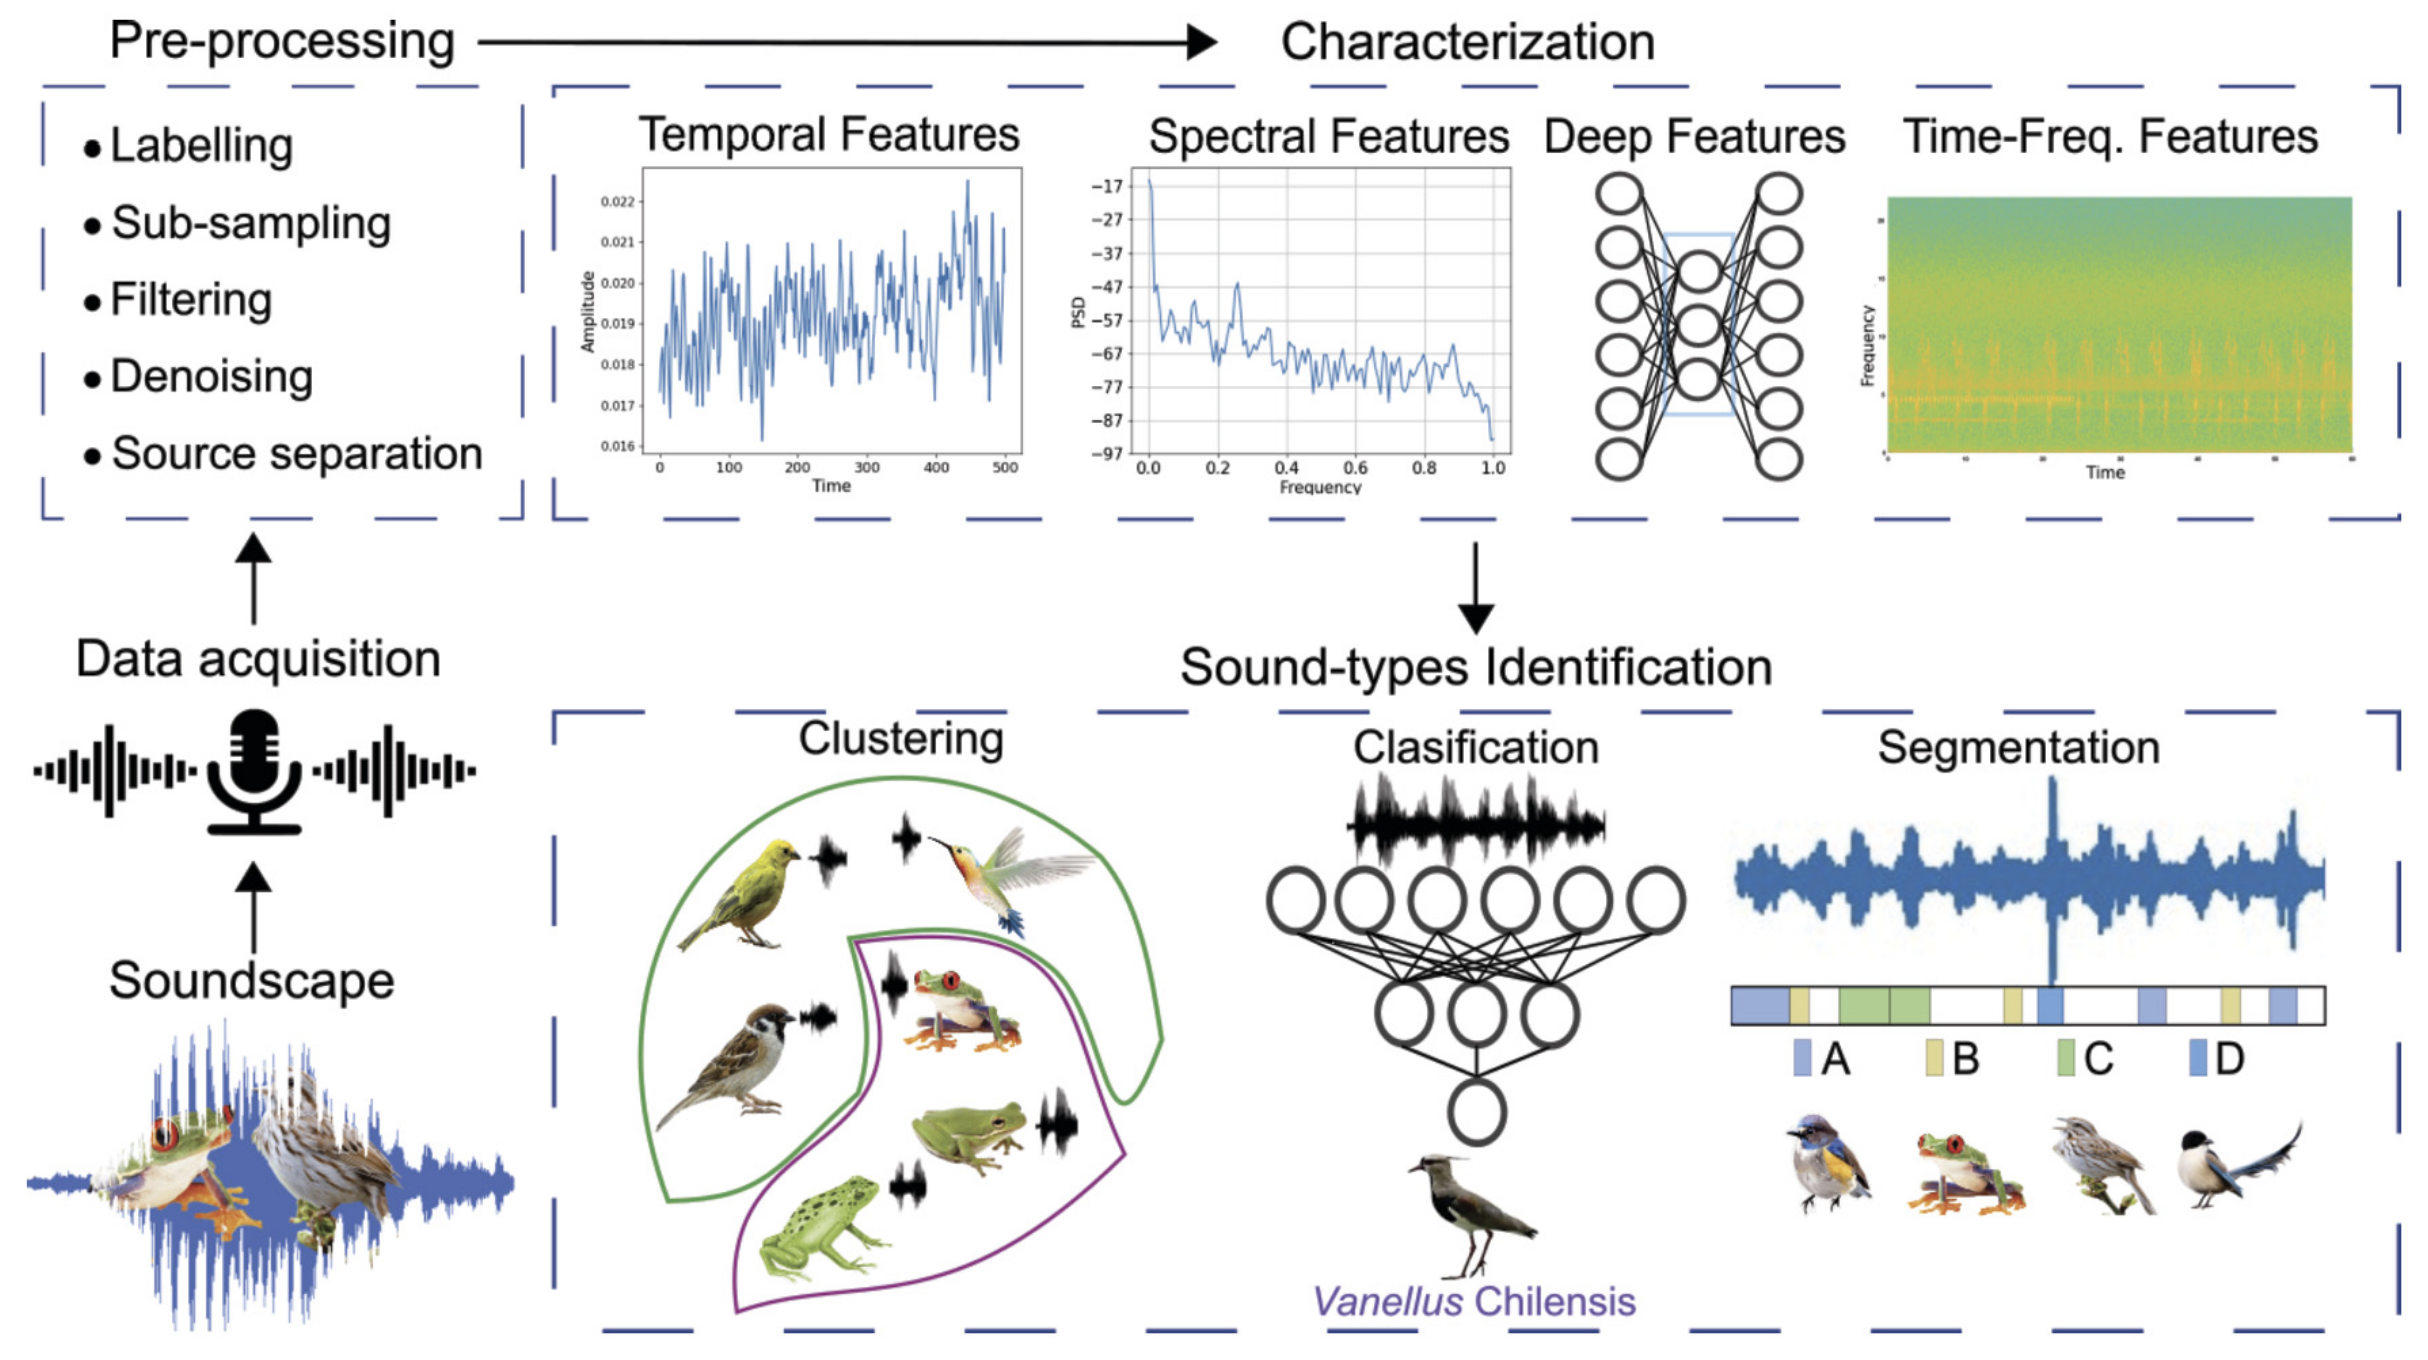
\includegraphics[width=0.95\textwidth]{images/soundscape_ecology_ml_frameworks.png}
		\caption[Soundscape-ecology workflow for ecoacoustic monitoring.]{Soundscape-ecology data processing workflow with machine-learning stages for ecoacoustic monitoring. Source: Nieto-Mora et al. \cite{nietomora2023systematic}.}
		\label{fig:soundscape_ecology_ml_workflow}
	\end{figure}

	In this context, the literature distinguishes several related but different tasks. Acoustic detection identifies whether a target class of events is present. Species classification determines which species generated the signal. Event segmentation defines temporal boundaries of vocalizations inside a recording. Ecological inference then uses these outputs to estimate indicators such as richness, occupancy, or temporal activity profiles. The distinction is important because model errors at early stages propagate downstream. A detection system with a high false-positive tendency can bias ecological indicators even when the classifier itself is strong. This is one of the reasons why recent studies increasingly evaluate complete analysis pipelines rather than isolated model components \cite{nietomora2023systematic,perezgranados2023birdnet}.

	\subsection{Automated Bird Sound Detection and Classification}
	The first broad milestone for modern bird audio detection was the Bird Audio Detection challenge, which made explicit the need for robust generalization across datasets, recording devices, and environmental conditions \cite{stowell2019birdaudiodetection}. The relevance of this work also is highlighted in the evaluation philosophy: models were compared under realistic domain shift, making clear that laboratory-level scores do not automatically transfer to field-level reliability.

	A second major milestone is BirdNET, a globally scoped bird recognition model that demonstrated that deep architectures, combined with task-specific training strategies, can support practical biodiversity workflows \cite{birdnet2021}. BirdNET is significant because it moved the field from proof-of-concept models toward operational analysis of long recordings at taxonomic scale. Successive studies then shifted from pure adoption to critical analysis, especially regarding confidence thresholds, precision--recall trade-offs, and context-dependent calibration policies \cite{perezgranados2023birdnet}. This line of work highlights that threshold selection is not a secondary technical parameter but an ecological design decision, since different monitoring goals require different error profiles.

	The classification literature also reports persistent data-related challenges. Public repositories provide large quantities of recordings, but label quality and class distribution are uneven. Many datasets are weakly labeled, highly imbalanced, and geographically heterogeneous, creating strong domain mismatch between training and deployment scenarios. This has motivated extensive use of augmentation, transfer learning, and domain adaptation. Recent work based on large pre-trained acoustic encoders confirms this trend, showing that strong representations can be transferred to bird classification when adaptation is carefully designed for class imbalance and non-stationary background conditions \cite{sheikh2024birdwhisperer}.

	\begin{figure}[H]
		\centering
		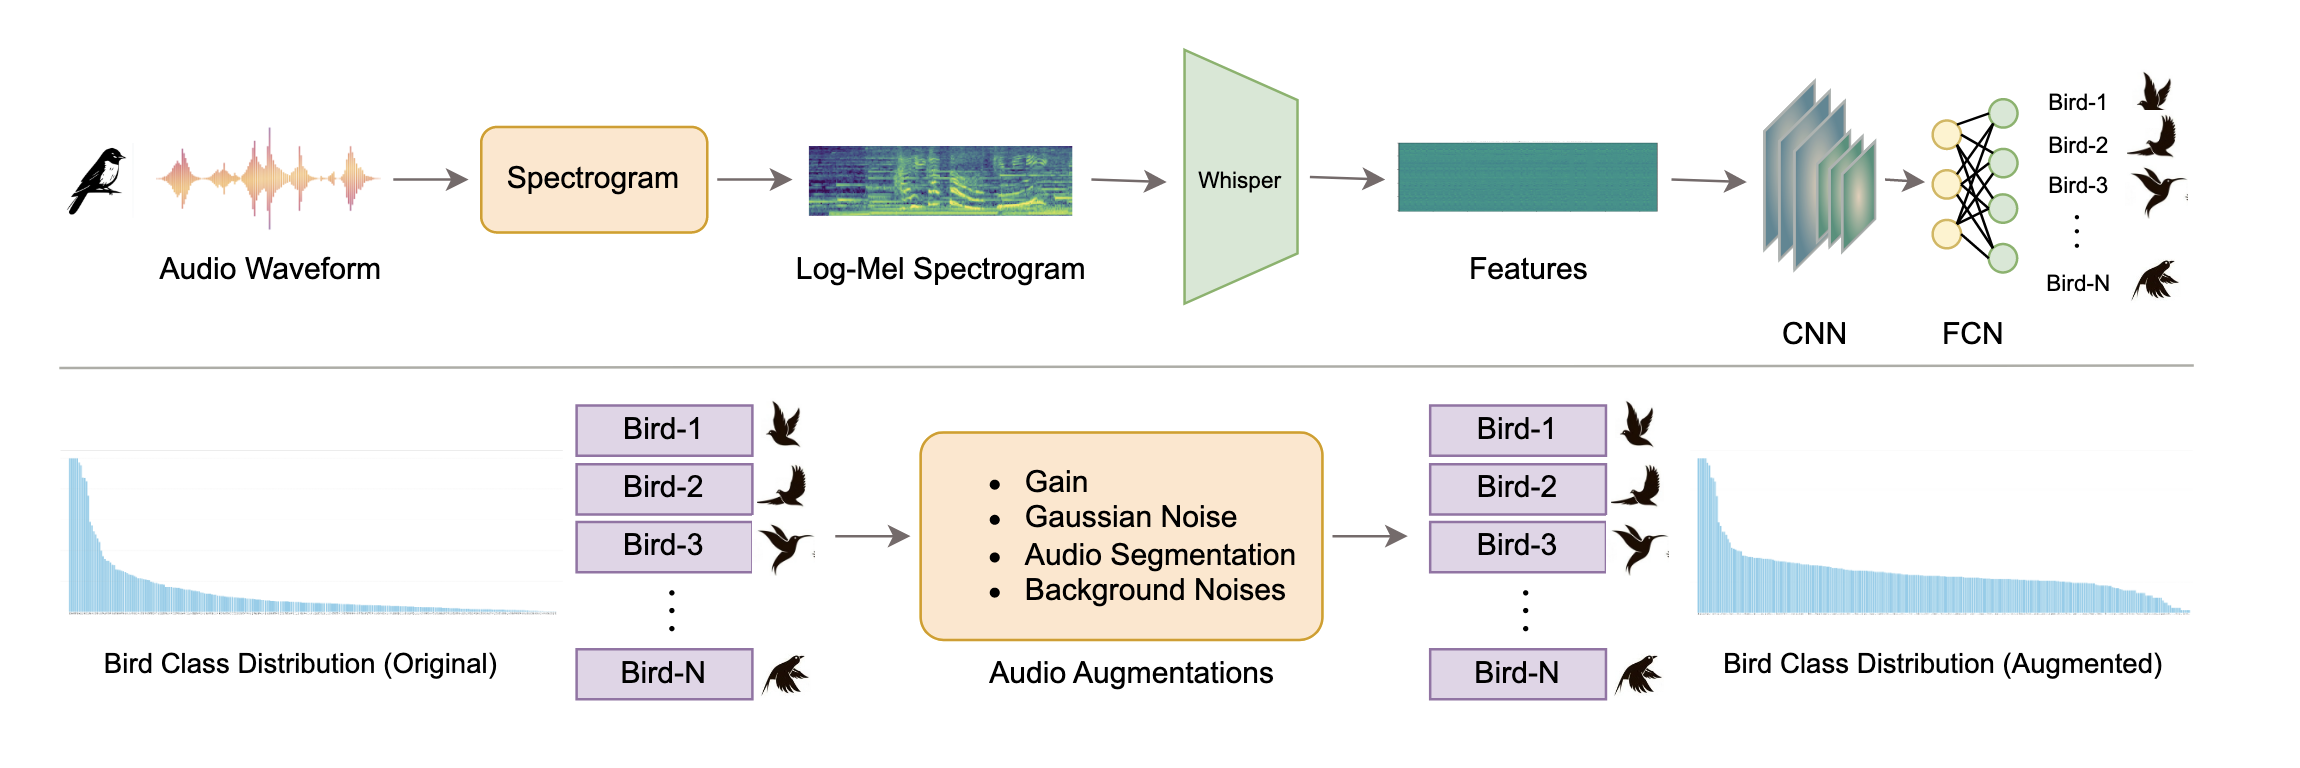
\includegraphics[width=0.95\textwidth]{images/birds_pipeline.png}
		\caption[Bird Whisperer methodology overview.]{Bird Whisperer methodology overview: top, classification pipeline from waveform spectrogram through encoder and compact prediction head; bottom, augmentation and class-imbalance mitigation workflow. Source: Sheikh et al. \cite{sheikh2024birdwhisperer}.}
		\label{fig:bird_whisperer_pipeline}
	\end{figure}

	\subsection{Cross-Domain Wildlife Monitoring Insights}
	Adjacent taxa, especially bats, provide useful methodological parallels for bird monitoring. Bat acoustic pipelines face severe constraints in bandwidth, event sparsity, and noise, yet they address the same structural problem of converting massive passive recordings into reliable ecological evidence. Deep-learning-based open pipelines for bat detection showed clear gains over traditional rule-based approaches under noisy conditions \cite{macaodha2018batdetective}. Subsequent IoT deployments demonstrated that edge-side filtering and event-centric transmission can drastically reduce storage and communication loads while preserving ecological utility \cite{gallacher2021shazam}.

	These results are relevant for bird monitoring because they reinforce a general principle: model quality must be evaluated jointly with acquisition strategy, compute placement, and downstream ecological use. In other words, recognition models are one component of a full cyber-physical monitoring system.

	\subsection{Edge AI and TinyML for Bioacoustics}
	Remote and long-duration deployments make edge computation a central requirement. Cloud-centric processing remains useful for retrospective analysis, but many field scenarios benefit from local inference to reduce energy, bandwidth, and memory pressure. TinyML literature addresses this requirement by designing models and runtimes for microcontroller-class devices.

	AudioMoth and similar devices made large-scale acoustic campaigns economically feasible, but they also exposed practical limits of continuous full-resolution logging \cite{audiomoth2019}. For this reason, always-on classifiers have become central in low-power ecoacoustics. Existing studies show that lightweight on-device classifiers can run for extended periods while preserving acceptable recognition quality, enabling selective storage and adaptive duty cycles \cite{sabbella2022alwayson,tinychirp2024}. The same direction is visible in broader AI-IoT architectures for bird monitoring, where communication infrastructure and model design are co-optimized for operational continuity \cite{seguragarcia2024}.

	Recent work also reports direct on-device identification on AudioMoth with a shallow neural classifier and explicit power profiling, further confirming the feasibility of real-time acoustic intelligence on logger-class hardware \cite{velascomontero2026onsite}. The same study is complementary in scope because it focuses on a single-species binary setting, while the present framework addresses compact multi-species classification.

		\begin{sloppypar}
		At architectural level, the literature converges around compact convolutional families based on depthwise-separable operations, residual paths, and scalable width/depth configurations. MobileNetV2 formalized key efficiency principles that later influenced many embedded audio systems \cite{mobilenetv2}. MatchboxNet translated these principles into 1D temporal processing for low-footprint keyword and sound recognition \cite{matchboxnet2020}. PhiNets and related scalable backbones further emphasized explicit resource-aware design spaces \cite{phinets2022,paissan2022scalableaudio}.
		\end{sloppypar}

	\subsection{Audio Representation and Learnable Front-Ends}
	The front-end representation used before high-level classification is another decisive design axis. Classical pipelines rely on fixed time--frequency transforms, usually STFT-derived spectrograms and mel-scaled filterbanks, because they provide stable and interpretable features. However, bird vocalizations present strong inter-species overlap and context-dependent spectral variability, which can limit purely fixed representations.

		\begin{sloppypar}
		This motivated the development of learnable or partially learnable front-ends. SincNet introduced constrained parameterized filters with clear physical interpretation, improving interpretability and parameter efficiency in waveform-based processing \cite{ravanelli2019sincnet}. LEAF further generalized learnable front-end design as a drop-in alternative to mel filterbanks and showed broad applicability across audio domains \cite{zeghidour2021leaf}. In parallel, discriminative and parametric filter-bank studies optimized center frequencies, bandwidths, gains, and filter shapes directly from data while preserving structural priors \cite{zhangwu2019discriminative,caiko2023parametric,peictukuljac2022learnable}.
		\end{sloppypar}

	This branch of literature is directly relevant for embedded bird classification because front-end choice affects both accuracy and deployment cost. A representation that is acoustically informative but computationally heavy may be unsuitable for long-term edge deployment, while a compact representation that misses discriminative details can fail on hard species subsets.

	\subsection{Compression and Training Strategies for Constrained Deployment}
		\begin{sloppypar}
		The constrained deployment literature repeatedly converges on the same point: compact architecture design and compression-aware training must be co-optimized, and performance must be assessed with real device metrics, not only with parameter count. Across studies, quantization, pruning, and distillation are the most recurrent techniques for obtaining deployable models under strict memory and power budgets \cite{wuint8quant2020,li2019pruning,hinton2015distilling}. Their practical impact, however, depends strongly on runtime kernels and hardware characteristics. For this reason, microcontroller-oriented analyses increasingly report latency, power, and energy jointly \cite{tao2022energy}.
		\end{sloppypar}

	\subsection{Synthesis and Research Gap}
	The reviewed literature shows a clear progression from isolated recognition models to integrated monitoring pipelines that must remain accurate, efficient, and robust under real field conditions. Existing work provides strong foundations in bird sound recognition, adaptive audio representations, and embedded inference. However, an important gap remains at their intersection.

	Current literature already includes relevant examples of bird-species recognition on edge platforms and a smaller set of low-power embedded classifiers. However, the evidence remains limited for compact \emph{multi-class} bird classifiers validated directly on microcontroller-class or logger-class hardware under strict memory and energy constraints. Existing studies often cover either broad species inventories executed on more capable edge platforms, or low-power embedded settings focused on binary detection or few-species classification \cite{sabbella2022alwayson,tinychirp2024,seguragarcia2024,velascomontero2026onsite}. This leaves comparatively less evidence on the joint problem of multi-species recognition, strict embedded deployment, and direct system-level validation on the final device.

	A second limitation concerns evaluation depth. A globally scoped bird recognition model such as BirdNET provides a strong reference for recognition quality \cite{birdnet2021}, but its design point is different from that of always-on microcontroller pipelines operating under tight energy and memory budgets. Conversely, many lightweight embedded studies emphasize feasibility and efficiency, but are often validated on simplified class sets, species-specific detection tasks, or settings with limited analysis of difficult inter-species confusions. Front-end adaptation studies are also frequently reported without complete deployment-level validation on low-power loggers \cite{zeghidour2021leaf,peictukuljac2022learnable,caiko2023parametric}.

	These limitations have an important design implication. Under strict energy, memory, and latency budgets, local specialization becomes a more realistic strategy than attempting fully general recognition on-device. In practical ornithological monitoring, target taxa, prevalence, and acoustic confounders are strongly site-dependent, because bird communities vary with landscape composition, habitat heterogeneity, and topo-climatic context \cite{birdnet2021,anderle2025drivers}. A classifier optimized for the species pool of a specific geographic area or campaign can therefore allocate its representational capacity where it is most useful. This improves practical discrimination in the deployment context instead of spending model budget on species that are not expected in that region \cite{birdnet2021}.

	This specialization is also operationally useful for large-scale deployment. By remaining compatible with small, low-power, and relatively inexpensive devices, the system can support wider deployment density, lower infrastructure cost, hardware repurposing across campaigns, and longer unattended monitoring in the field. When inference is executed directly on a low-power logger, battery autonomy can support longer deployments and reduce the need for frequent retrieval trips in remote sites \cite{audiomoth2019,tinychirp2024}. In addition, first-pass on-device classification can reduce storage pressure and manual re-analysis workload by prioritizing the most informative parts of the acoustic stream for expert review \cite{gallacher2021shazam,sabbella2022alwayson}.

	To the best of our knowledge, practical end-to-end frameworks that jointly combine a semi-learnable front-end, a compact temporal model specialized for local species sets, and direct on-device benchmarking with explicit energy comparison against strong baselines remain limited in bird-monitoring literature. This thesis addresses that gap by developing a practical end-to-end framework for multi-species bird classification on low-power bioacoustic loggers under a unified system-level evaluation protocol.

	\chapter{Study and Implementation}
	This chapter presents the methods introduced in this thesis and treats representation learning, compact modeling, and deployment profiling as one integrated engineering problem.
	The proposed system combines established building blocks from the literature with original contributions targeted at low-power bioacoustic monitoring. The standard part of the architecture includes STFT-based time-frequency analysis, a compact temporal convolutional backbone, GRU temporal modeling, and attention pooling.

	Relative to common fixed front-end pipelines discussed in Chapter~1, the main contributions of this study are:
	\begin{itemize}
		\item a semi-learnable front-end that preserves an interpretable log--linear prior while adapting frequency allocation to the active species set;
		\item a small and specialized model configuration, explicitly optimized for difficult local species subsets instead of generic large-scale taxonomies;
		\item a complete deployment path on AudioMoth, including firmware-side integration and on-device latency/energy benchmarking;
		\item a reproducible experimental pipeline with realistic negative-class modeling and controlled comparisons among fixed, semi-learnable, and fully learnable front-end strategies.
	\end{itemize}
	\section{System Study and Implementation}
	\subsection{Problem Definition and Project Scope}
	The project addresses \emph{multi-class bird sound classification}. Multi-class classification means that, given one input clip \(x\), the model must select exactly one label among \(C\) possible classes. In this work, the classes are bird species plus one additional negative class representing the absence of bird vocalizations. If \(p(c \mid x)\) denotes the predicted probability for class \(c\), the decision is made by selecting the class associated with the highest probability.

	What makes bird sound classification difficult, apart from the number of classes, is the acoustic structure of bird vocalizations. Some species are highly distinctive and occupy relatively specific frequency regions. Other species are acoustically close, especially when they belong to the same family or when their calls are short, weak, or partially masked by background noise. The same species can also vary strongly across individuals, seasons, distances from the microphone, and behavioral context. In practice, this creates a simultaneous inter-class overlap problem and intra-class variability problem.

	The project also targets edge deployment, where memory, latency, and energy are constrained \cite{audiomoth2019}. This changes the design objective. The model is optimized to combine high accuracy, robustness, compact size, and low energy cost. For this reason, the system is designed as a compact end-to-end architecture with a carefully structured spectral front-end and a training strategy that transfers knowledge from a stronger teacher model \cite{birdnet2021,hinton2015distilling}.

	\subsection{Dataset}
	\subsubsection{Dataset Composition and Class Definition}
		The training set merges species-labeled bird recordings, environmental sounds, and silence-only segments, so the model learns both species discrimination and reliable ``no-bird'' rejection. Positive classes correspond to bird species, and each sample in these classes contains a vocal event that should be recognized as one label among many possible species. The central practical requirement is a \emph{closed-set multi-class decision}: for each 3-second audio window, the model must output one class index from the available species set plus one additional class that represents the absence of bird vocalizations.

	\subsubsection{Data Sources and API Queries}
	Bird-positive material is collected from species-labeled field recordings, with Xeno-canto serving as a major source of realistic recording variability \cite{xenocanto}. Different microphones, habitats, propagation distances, weather conditions, and background acoustic scenes broaden the observed training distribution. In practice, this functions as a form of natural augmentation, exposing the model to realistic background noise and acquisition conditions that improve robustness at deployment time. As a result, a model trained only on acoustically clean or homogeneous examples would be poorly matched to real monitoring scenarios.

	Environmental audio from ESC-50 is integrated to represent realistic non-bird acoustic conditions \cite{esc50}. This source supports two key functions. First, it helps construct a robust negative class that prevents systematic false alarms. Second, it provides a diverse background library for augmentation, so bird calls can be learned under controlled interference levels. In passive monitoring, the majority of windows contains no target vocalization, therefore the ``no bird'' class is a structural component of the task and not an auxiliary engineering trick.

	The acquisition stage is large-scale. An automated query pipeline collects raw field recordings for the selected species and yields 150,645 downloaded files before quality filtering and clip extraction. After mono conversion, resampling, validation checks, and fixed-length clip construction, the effective corpus used for training and evaluation contains 150,557 clips of 3 seconds each.

	\subsubsection{Species Coverage and Subset Strategy}
	The complete species pool used in the project contains seventy bird classes, to which an explicit ``no bird'' class is added in training and evaluation. The full inventory covers raptors, owls, swifts, swallows, woodpeckers, treecreepers, tits, warblers, thrushes, finches, corvids, and other passerines, thus exposing the model to broad ecological and acoustic diversity.

	The complete species pool is shown visually in Figure~\ref{fig:species_pool_atlas}, which provides a photographic atlas of the seventy modeled bird species. This is more readable than listing all taxa inline and also makes the coverage of ecological groups and vocal profiles easier to inspect at a glance.

	\clearpage
	\makeatletter
\setlength{\@fptop}{0pt}
\makeatother
\begin{figure}[p]
\centering
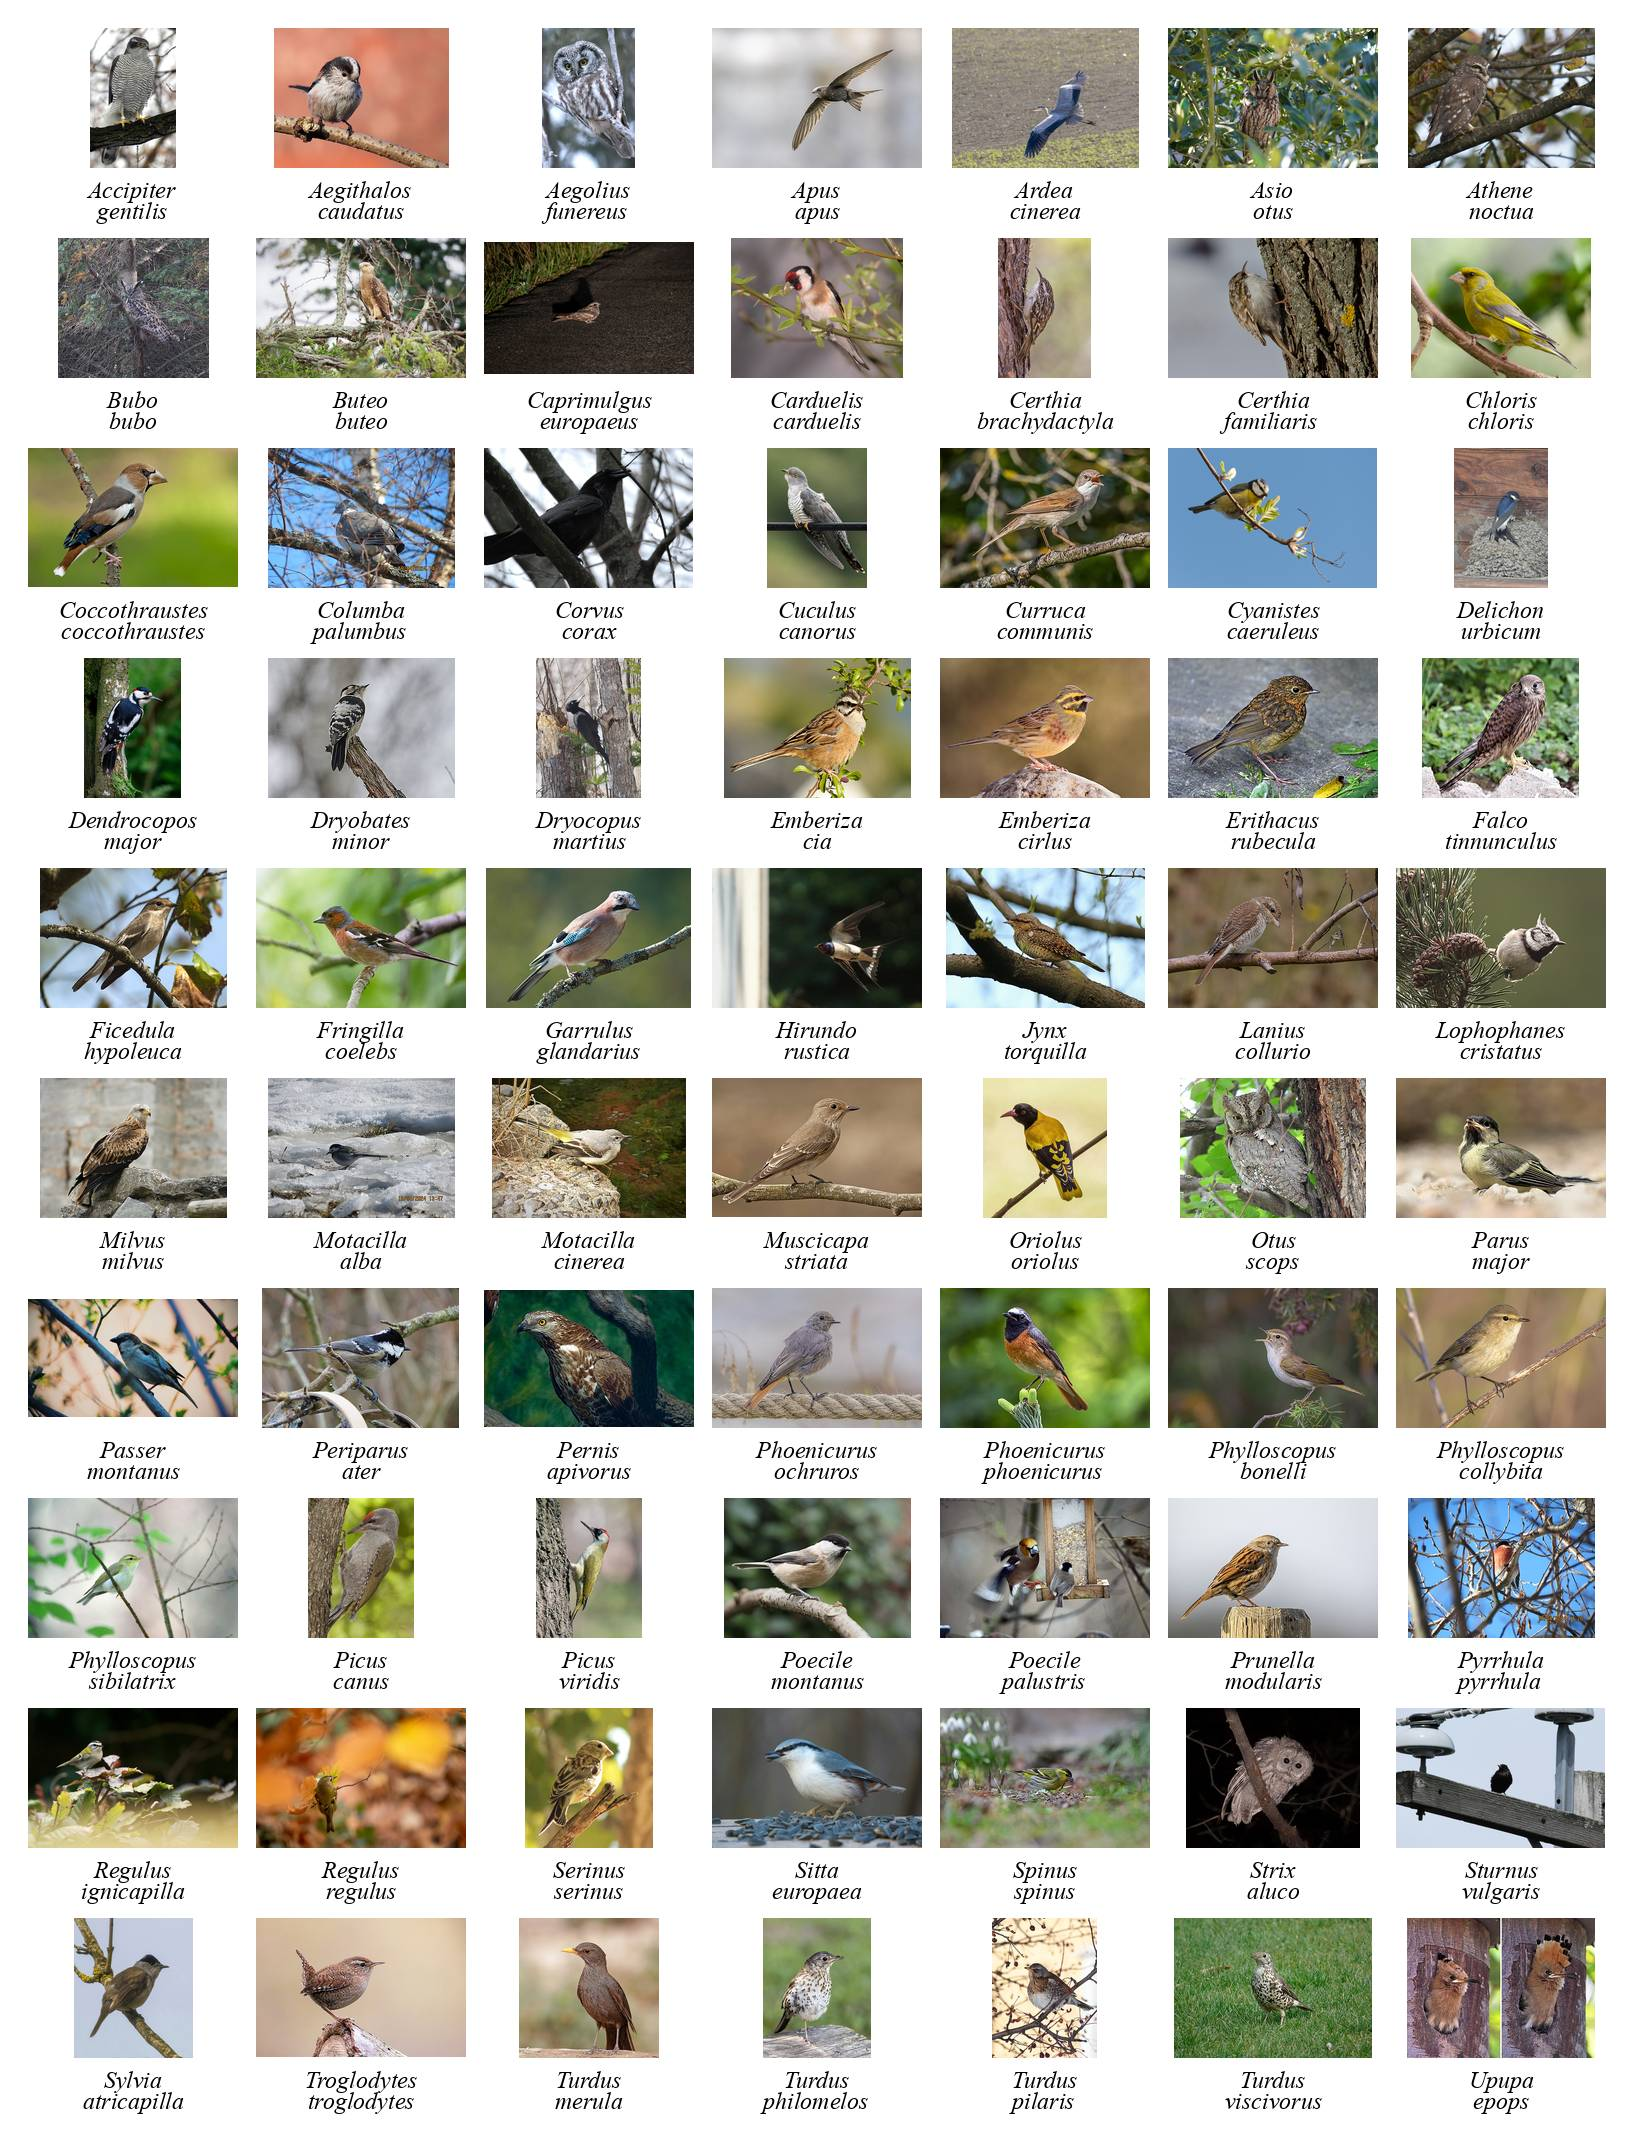
\includegraphics[width=\textwidth]{images/generated/bird_species_atlas.jpg}
\caption[Photographic atlas of the species pool.]{Photographic atlas of the species pool used in this thesis. Photo sources: Wikimedia Commons.}
\label{fig:species_pool_atlas}
\end{figure}

	\clearpage

	Beyond full-pool training, the experimental data consists of targeted subsets to isolate specific difficulty factors. These subset definitions were chosen by discussing and refining them with the ornithologists at Eurac involved in the project, so that the selected species groups represent ecological and acoustic difficulty patterns. A core \(8(+1)\) subset (\emph{Poecile montanus}, \emph{Certhia familiaris}, \emph{Apus apus}, \emph{Bubo bubo}, \emph{Periparus ater}, \emph{Emberiza cia}, \emph{Lophophanes cristatus}, \emph{Certhia brachydactyla}, plus ``no bird'') is used for direct front-end comparisons, including semi-learnable versus fully learnable variants under matched conditions. An ``easy species'' \(8(+1)\) subset (\emph{Ardea cinerea}, \emph{Corvus corax}, \emph{Falco tinnunculus}, \emph{Hirundo rustica}, \emph{Otus scops}, \emph{Phylloscopus collybita}, \emph{Picus canus}, \emph{Strix aluco}) is used to characterize upper-bound behavior when class separation is more favorable. A ``hard species'' \(13(+1)\) subset is designed around known confusions, including close taxonomic or acoustic pairs such as \emph{Parus major}/\emph{Periparus ater}, \emph{Regulus regulus}/\emph{Regulus ignicapilla}, and \emph{Certhia familiaris}/\emph{Certhia brachydactyla}, together with multiple \emph{Turdus} species and additional confounders.

	Additional subset studies include monoclass settings, a two-class hard-couple setting focused on the two \emph{Regulus} species, and frequency-focused subsets. The high-frequency-focused subset includes \emph{Serinus serinus}, \emph{Prunella modularis}, \emph{Regulus ignicapilla}, \emph{Troglodytes troglodytes}, and \emph{Apus apus}; the low-frequency-focused subset is centered on species such as \emph{Caprimulgus europaeus}, \emph{Corvus corax}, \emph{Upupa epops}, and \emph{Ardea cinerea}. The methodological reason for this subset design is controlled analysis: each subset emphasizes one dominant factor, such as inter-class similarity, spectral-region dependence, or negative-class calibration, so architectural and loss-function effects can be interpreted with less confounding than in full-pool training alone.

	This design is also consistent with recent species-level threshold analyses in passive acoustic monitoring. In an Alpine case study based on 25 hours of expert-annotated recordings and 17,737 bird sounds, Scanferla et al. derived 72 species-specific BirdNET decision thresholds and showed that precision varies substantially across species \cite{scanferla2025thresholds}. More specifically, the cited work models thresholds on BirdNET scores so that detections are accepted only above a chosen cutoff. For confidence-based thresholding, the paper reports species-specific thresholds for target precision levels of 0.90, 0.95, and 0.99, denoted \(ct0.90\), \(ct0.95\), and \(ct0.99\). It also evaluates analogous thresholds on the underlying unbounded logit score. Threshold choice can therefore affect species unevenly even when the same globally scoped bird recognition model is used. Figure~\ref{fig:scanferla_thresholds_species} illustrates this heterogeneity across many species, while Figure~\ref{fig:scanferla_thresholds_example} shows, for one species, how confidence-threshold and logit-threshold formulations lead to different operating points. These results are useful here because they reinforce the need for subset-based analysis, difficult-species inspection, and explicit calibration rather than assuming uniform behavior across the entire species pool.

	\begin{figure}[H]
		\centering
		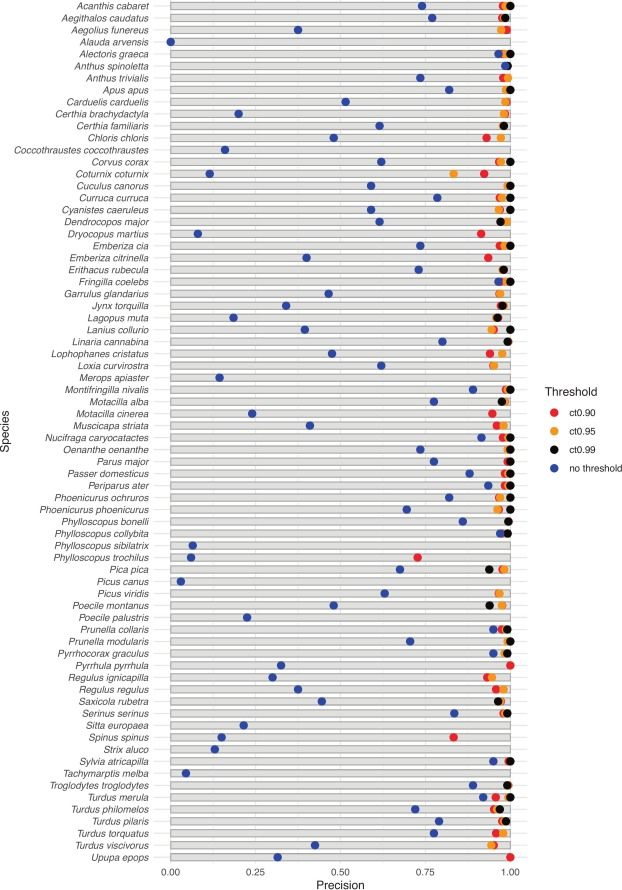
\includegraphics[width=0.72\textwidth]{images/scanderla/1-s2.0-S1574954125004327-gr3.jpg}
		\caption[Species-level precision after BirdNET threshold calibration.]{Species-level precision achieved after applying species-specific BirdNET confidence thresholds in passive acoustic monitoring. The colors correspond to thresholds chosen to target different precision levels in the cited study: \(ct0.90\), \(ct0.95\), and \(ct0.99\), while the blue reference indicates the original BirdNET precision without thresholding. The figure shows that the same thresholding strategy does not affect all species equally: some species already have high baseline precision, whereas others improve substantially only after species-specific threshold calibration \cite{scanferla2025thresholds}.}
		\label{fig:scanferla_thresholds_species}
	\end{figure}

	\begin{figure}[H]
		\centering
		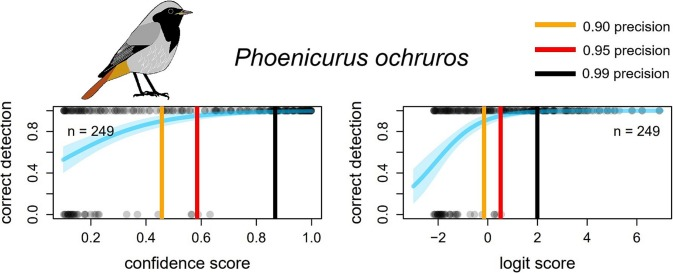
\includegraphics[width=0.82\textwidth]{images/scanderla/1-s2.0-S1574954125004327-gr2.jpg}
		\vspace{0.6em}
		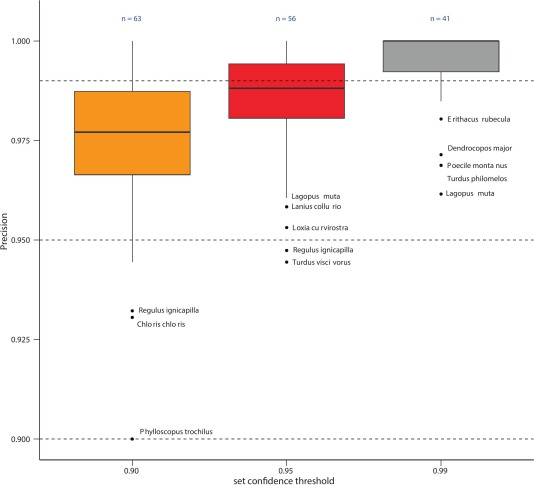
\includegraphics[width=0.62\textwidth]{images/scanderla/1-s2.0-S1574954125004327-gr4.jpg}
		\caption[Illustrative BirdNET threshold modeling and precision summary.]{Illustrative BirdNET threshold modeling from the external passive-acoustic study. Top: for \emph{Phoenicurus ochruros}, logistic-regression models are fitted using either BirdNET confidence score or the underlying logit score, and the intersections with the target precision levels 0.90, 0.95, and 0.99 define the corresponding decision thresholds. Bottom: boxplot summary of the precision obtained after applying species-specific confidence thresholds across the study species. Together, the two panels show both how an individual threshold is computed and why threshold calibration must be species-aware rather than globally fixed \cite{scanferla2025thresholds}.}
		\label{fig:scanferla_thresholds_example}
	\end{figure}

	\subsubsection{Negative-Class Construction and Balancing Strategy}
	The negative class is constructed from two complementary acoustic populations. The first population contains environmental sounds with no bird target, sampled from selected ESC-50 categories that include both natural contexts and anthropogenic disturbances. In practice, a focused subset of fourteen categories is used so the acoustic conditions remain realistic for field monitoring. The second population contains acoustically empty segments extracted directly from bird-recording sessions. This second source is essential because it captures recorder-specific floor noise, wind texture, distant background communities, and site-dependent silence profiles that are typically absent from curated environmental datasets.

	Using both sources avoids a degenerate ``no bird'' prototype. If negatives came only from external environmental datasets, the model could overfit to dataset identity rather than to the semantic concept ``no target bird vocalization''. If negatives came only from in-domain silence, it could remain weak against structured non-bird events such as rain bursts, traffic components, or mechanical sounds. A balanced mixture of environmental and empty-segment negatives gives broader coverage and reduces brittle decision boundaries.

	The dataset can be assembled in a static mode or in a dynamic mode. In static mode, a pre-built negative pool is reused across runs to maximize reproducibility during controlled comparative studies. In dynamic mode, negatives are regenerated during loading, increasing stochastic diversity across epochs. In the default setting, environmental negatives and empty-segment negatives are combined with a 50:50 ratio before final class balancing. The number of negatives is then controlled by matching it to the average number of examples per bird class:
	\begin{equation}
		N_{\mathrm{neg}}^{\star} = \frac{1}{K}\sum_{k=1}^{K} N_k,
	\end{equation}
	where \(K\) is the number of bird species classes and \(N_k\) is the sample count of class \(k\). This rule keeps optimization pressure comparable between bird and non-bird decisions without forcing artificial uniformity across all species.

	When one source provides fewer negatives than expected, the balancing stage applies a controlled fallback strategy that preserves training continuity and keeps the resulting class composition explicit. This avoids hidden ratio drift and improves comparability across experiments.

	\subsubsection{Preprocessing}
	All sources are transformed into a common representation before any learning stage. Stereo recordings are converted to mono to remove channel inconsistency, then resampled to 32~kHz and mapped to fixed 3-second windows. A fixed temporal support is required by the neural architecture and also stabilizes batching, memory allocation, and gradient statistics during training.

	The preprocessing stage also handles common field-data quality problems. Input validity is checked before feature extraction, and malformed or unreadable recordings are managed through controlled fallback behavior so that isolated file failures do not interrupt long training runs. The same normalization policy is applied across common recording formats, allowing heterogeneous acquisition campaigns to be merged into a coherent dataset.

	For positive samples, segmentation is call-centered rather than random. The signal is first band-pass filtered in the range 150--16,000~Hz, which suppresses irrelevant very-low-frequency drift and high-frequency artifacts while preserving the dominant spectral support of bird vocalizations. An amplitude envelope is then computed on short overlapping windows, typically 50~ms with 10~ms hop, to obtain a robust temporal trace of acoustic salience.

	Peak selection uses adaptive statistics so thresholds follow each recording rather than being fixed globally. Prominence is estimated through the median and the median absolute deviation (MAD):
	\begin{equation}
		\theta_{\mathrm{prom}} = \mathrm{median}(e) + 1.5\,\mathrm{MAD}(e),
	\end{equation}
	where \(e\) is the envelope sequence. A minimum peak distance of approximately 1 second prevents repeated detections of the same vocal event, and percentile filtering (for example around the upper quartile of peak heights) discards weak candidates that are unlikely to contain discriminative species information. Each selected event is centered inside the 3-second crop to maximize informative content. When no reliable peak is found, a deterministic fallback segment is extracted from the initial part of the recording, so the pipeline remains robust and does not fail on low-energy or weakly vocal clips.

	Empty-segment extraction follows the same statistical philosophy. Frame-level energy is estimated and low-activity intervals are selected through robust thresholds, avoiding fragile absolute cutoffs. A practical rule is
	\begin{equation}
		\theta_{\mathrm{sil}} = 0.5 \cdot \mathrm{median}(E),
	\end{equation}
	with \(E\) denoting frame-level energy. Candidate segments are separated in time to avoid highly redundant crops, and per-recording extraction can be capped (for example to five segments) to prevent very quiet recordings from dominating the negative pool. Segment management is pooled and seed-controlled so reuse remains efficient while preserving split isolation and diversity. This procedure yields realistic negatives that preserve ambient acoustic identity, unlike synthetic zero-signal segments.

	\begin{figure}[H]
		\centering
		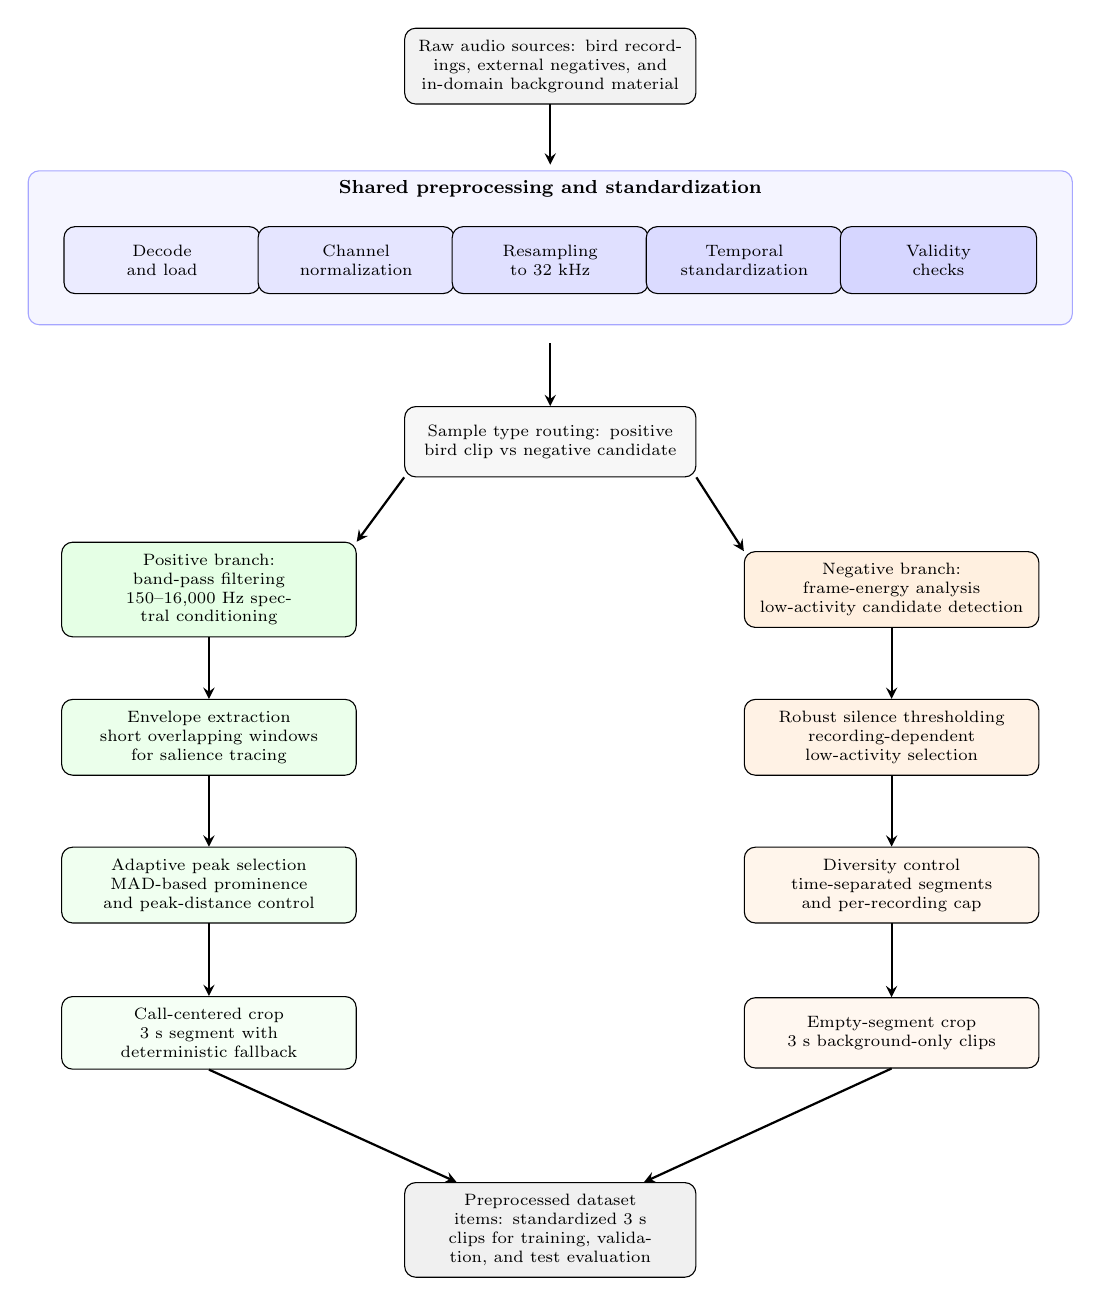
\begin{tikzpicture}[
			x=1cm,
			y=0.92cm,
			>=stealth,
			scale=0.85,
			transform shape,
			font=\scriptsize,
			box/.style={draw, rounded corners, align=center, minimum height=1.0cm, text width=2.65cm, inner sep=4pt},
			widebox/.style={draw, rounded corners, align=center, minimum height=1.05cm, text width=4.0cm, inner sep=5pt},
			branchbox/.style={draw, rounded corners, align=center, minimum height=1.05cm, text width=4.05cm, inner sep=5pt}
		]
			\node[widebox, fill=gray!10] (input) at (0,0) {Raw audio sources: bird recordings, external negatives, and in-domain background material};

			\draw[rounded corners, fill=blue!4, draw=blue!35] (-7.8,-4.2) rectangle (7.8,-1.7);
			\node[font=\footnotesize\bfseries, text=black] at (0,-2.0) {Shared preprocessing and standardization};
			\node[box, fill=blue!8]  (decode)    at (-5.8,-3.15) {Decode\\and load};
			\node[box, fill=blue!10] (mono)      at (-2.9,-3.15) {Channel\\normalization};
			\node[box, fill=blue!12] (resample)  at (0.0,-3.15) {Resampling\\to 32 kHz};
			\node[box, fill=blue!14] (windowing) at (2.9,-3.15) {Temporal\\standardization};
			\node[box, fill=blue!16] (validity)  at (5.8,-3.15) {Validity\\checks};

			\node[widebox, fill=gray!6] (routing) at (0,-6.1) {Sample type routing: positive bird clip vs negative candidate};

			\node[branchbox, fill=green!10] (pos1) at (-5.1,-8.5) {Positive branch:\\band-pass filtering\\150--16{,}000 Hz spectral conditioning};
			\node[branchbox, fill=green!8]  (pos2) at (-5.1,-10.9) {Envelope extraction\\short overlapping windows\\for salience tracing};
			\node[branchbox, fill=green!6]  (pos3) at (-5.1,-13.3) {Adaptive peak selection\\MAD-based prominence\\and peak-distance control};
			\node[branchbox, fill=green!4]  (pos4) at (-5.1,-15.7) {Call-centered crop\\3 s segment with\\deterministic fallback};

			\node[branchbox, fill=orange!12] (neg1) at (5.1,-8.5) {Negative branch:\\frame-energy analysis\\low-activity candidate detection};
			\node[branchbox, fill=orange!10] (neg2) at (5.1,-10.9) {Robust silence thresholding\\recording-dependent\\low-activity selection};
			\node[branchbox, fill=orange!8]  (neg3) at (5.1,-13.3) {Diversity control\\time-separated segments\\and per-recording cap};
			\node[branchbox, fill=orange!6]  (neg4) at (5.1,-15.7) {Empty-segment crop\\3 s background-only clips};

			\node[widebox, fill=gray!12] (output) at (0,-18.9) {Preprocessed dataset items: standardized 3 s clips for training, validation, and test evaluation};

			\draw[->, thick] (input.south) -- (0,-1.6);

			\draw[->, thick] (0,-4.5) -- (routing.north);

			\draw[->, thick] (routing.south west) -- (pos1.north east);
			\draw[->, thick] (routing.south east) -- (neg1.north west);

			\draw[->, thick] (pos1.south) -- (pos2.north);
			\draw[->, thick] (pos2.south) -- (pos3.north);
			\draw[->, thick] (pos3.south) -- (pos4.north);

			\draw[->, thick] (neg1.south) -- (neg2.north);
			\draw[->, thick] (neg2.south) -- (neg3.north);
			\draw[->, thick] (neg3.south) -- (neg4.north);

			\draw[->, thick] (pos4.south) -- ([xshift=-1.4cm]output.north);
			\draw[->, thick] (neg4.south) -- ([xshift=1.4cm]output.north);
		\end{tikzpicture}
		\caption[Detailed preprocessing pipeline.]{Detailed preprocessing pipeline. All audio first passes through shared standardization, then the pipeline branches into call-centered extraction for positive samples and low-activity empty-segment extraction for negative samples, producing standardized 3-second clips for training and evaluation.}
		\label{fig:preprocessing_pipeline_blocks}
	\end{figure}

	\subsubsection{Dataset Split Policy and Effective Usage During Training}
	Data partitioning is fixed and reproducible. The standard split uses 70\% of data for training, 15\% for validation, and 15\% for testing, with deterministic seeding so experimental comparisons remain scientifically valid. Label indexing is deterministic as well: species classes occupy a stable index range and ``no bird'' is appended as an explicit additional class.

	Environmental data are split with leakage control. ESC-50 fold allocation is aligned with the global partition strategy, with folds 1--3 used in training, fold 4 in validation, and fold 5 in testing. This design limits the risk that near-duplicate background structures appear across train and evaluation phases.

	Only training samples pass through stochastic augmentation. Validation and test flows remain deterministic and acoustically faithful to the split content. This is essential for attribution: if evaluation were also augmented, measured differences between architectures or losses would be confounded by random transformation noise rather than reflecting true generalization changes.

	\subsubsection{Stochastic Acoustic Augmentation and SNR-Controlled Mixing}
	Augmentation is applied online during training to maximize diversity without inflating storage with pre-rendered variants. For each sample, up to two random transformations are composed, which is a compromise between robustness and acoustic plausibility. Temporal transformations include circular time shifts up to roughly \(\pm 10\%\) of clip duration and mild speed perturbation in the range 0.95--1.05. Spectral transformations include time masking (up to about 30 frames), frequency masking (up to about 10 bins), and low-level additive Gaussian noise with standard deviation around 0.01.

	Time masking hides short temporal intervals in the time--frequency representation, forcing the model to recognize species cues from incomplete evidence. Frequency masking hides narrow spectral bands, reducing reliance on single-bin artifacts and encouraging distributed feature use. Gaussian noise injection approximates electronic and environmental noise floors and improves tolerance to low-SNR recordings.

	Background mixing is the most deployment-relevant augmentation. Target bird clips are mixed with environmental audio at controlled signal-to-noise ratio, typically sampled in the range 5--15~dB. SNR is defined as
	\begin{equation}
		\mathrm{SNR}_{\mathrm{dB}} = 10 \log_{10}\!\left(\frac{P_{\mathrm{signal}}}{P_{\mathrm{noise}}}\right).
	\end{equation}
	To enforce a target SNR, the background waveform is power-scaled before summation:
	\begin{equation}
		\alpha = \sqrt{\frac{P_{\mathrm{signal}}}{P_{\mathrm{noise}} \cdot 10^{\mathrm{SNR}_{\mathrm{dB}}/10}}}, \qquad
		x_{\mathrm{mix}} = x_{\mathrm{signal}} + \alpha\,x_{\mathrm{noise}}.
	\end{equation}
	Background clips are cropped or tiled to match 3 seconds, and random offsets are used so the model does not repeatedly observe the same alignment patterns. The environmental pool includes both natural contexts (such as wind, rain, and water-related sounds) and anthropogenic contexts (such as traffic-like mechanical components), so robustness is learned across heterogeneous interference types. High-SNR cases preserve fine call detail, while low-SNR cases teach resilience to masking and overlap.

		\begin{sloppypar}
		When frequency-domain augmentations are applied, the pipeline preserves consistency between spectral edits and waveform-domain training input. Dynamic-range control in decibel space and phase-consistent reconstruction are used where needed to avoid acoustically implausible artifacts that could destabilize optimization.
		\end{sloppypar}

	The pipeline works because it aligns statistical training conditions with operational reality. Call-centered extraction increases the information density of positive examples, which improves sample efficiency for compact models. The dual-source negative class reduces false positives by teaching both structured environmental distractors and recorder-specific quiet conditions. Controlled augmentation expands the effective support of the training distribution without breaking acoustic plausibility.

	For edge deployment, this alignment directly determines field reliability. Compact models have little spare capacity to absorb domain shift between curated training clips and unattended real-world recordings. Training with heterogeneous backgrounds, explicit silence examples, and controlled SNR conditions makes runtime behavior more predictable, keeps false triggers low, and improves decision stability during long monitoring campaigns.

	\subsection{Semi-Learnable Filter Design}
	\label{sec:semi_learnable_filter_design}
	\subsubsection{Why a Semi-Learnable Front-End}
	Audio classification models operate on waveform samples and first map them to a time--frequency representation, where spectral patterns can be modeled over time. In bird bioacoustics, a fully fixed spectral mapping can be too rigid because species cues are distributed differently across frequency bands, recording conditions, and subsets of classes. As a result, a single predefined scale may allocate too much resolution to some regions and too little to others.

	A fully learnable front-end increases flexibility but can be harder to optimize and more prone to overfitting, especially under constrained-data or constrained-compute settings. The semi-learnable design used here keeps a structured and interpretable filterbank based on triangular filters, while learning only a small set of global parameters that control how spectral resolution is distributed. This preserves strong inductive bias and enables task-specific adaptation at the same time.

	\subsubsection{Mathematical Formulation}
	Let \(N\) be the number of filters and \(x_i=\frac{i}{N-1}\) the normalized filter index. Two frequency mappings are defined. The first one is logarithmic,
	\begin{equation}
		f_{\log}(x_i)=f_{\min}\left(\frac{f_{\max}}{f_{\min}}\right)^{x_i},
	\end{equation}
	and the second one is linear,
	\begin{equation}
		f_{\mathrm{lin}}(x_i)=f_{\min}+x_i(f_{\max}-f_{\min}).
	\end{equation}
	The model combines these two mappings through a sigmoid gate:
	\begin{equation}
		S(x_i;b,w)=\sigma\!\left(\left(x_i-\frac{b-f_{\min}}{f_{\max}-f_{\min}}\right)w\right),
	\end{equation}
	where
	\begin{equation}
		\sigma(z)=\frac{1}{1+e^{-z}}.
	\end{equation}
	Here \(b\) is the breakpoint and \(w\) is the transition width. The final center frequency of each filter is
	\begin{equation}
		f_i=(1-S(x_i;b,w))\,f_{\log}(x_i)+S(x_i;b,w)\,f_{\mathrm{lin}}(x_i).
	\end{equation}
	These centers define a triangular filterbank applied to STFT magnitudes. Let \(X_t(k)\) be the STFT magnitude at time frame \(t\) and frequency bin \(k\), and let \(H_m(k;b,w)\) denote filter \(m\). The filtered representation is
	\begin{equation}
		Z_m(t)=\sum_{k} H_m(k;b,w)\,X_t(k).
	\end{equation}
	After filtering, the representation is converted to decibel scale with bounded dynamic range and normalized per clip:
	\begin{equation}
		\tilde{Z}=\frac{Z_{\mathrm{dB}}-\mu}{\sigma+10^{-5}},
	\end{equation}
	with \(\mu\) and \(\sigma\) computed on the current sample. This step reduces scale variability across recordings and stabilizes optimization. The implementation also includes a frequency-axis alignment safeguard that resamples spectrogram channels to the expected front-end dimensionality when needed, so the downstream encoder always receives a consistent tensor geometry.
	Since \(b\) and \(w\) are differentiable parameters, gradients from the final classification loss can update the spectral allocation.

	\begin{figure}[H]
		\centering
		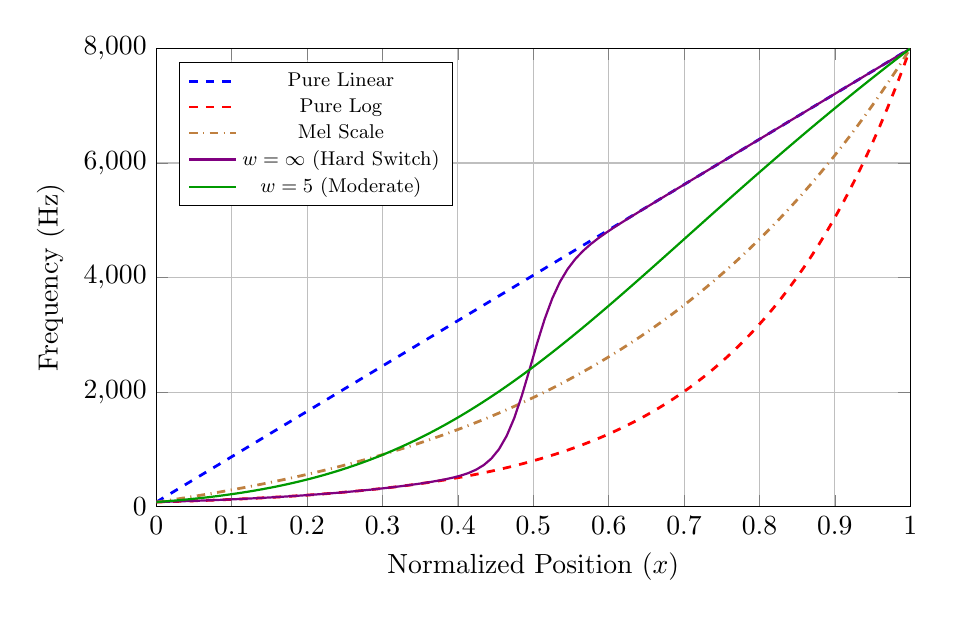
\begin{tikzpicture}
			\begin{axis}[
				width=0.92\textwidth,
				height=7.4cm,
				xlabel={Normalized Position (\(x\))},
				ylabel={Frequency (Hz)},
				xmin=0, xmax=1,
				ymin=0, ymax=8000,
				grid=major,
				legend pos=north west,
				legend style={font=\small, nodes={scale=0.8, transform shape}},
				samples=100
			]
				\def\fmin{80}
				\def\fmax{8000}
				\def\breakPoint{4000}
				\def\alphaVal{(\breakPoint - \fmin)/(\fmax - \fmin)}
				
				\addplot[blue, dashed, domain=0:1, line width=1pt]
				{\fmin + x*(\fmax - \fmin)};
				\addlegendentry{Pure Linear}
				
				\addplot[red, dashed, domain=0:1, line width=1pt]
				{\fmin * (\fmax/\fmin)^x};
				\addlegendentry{Pure Log}
				
				\addplot[brown, dash dot, domain=0:1, line width=1pt]
				{700 * (10^( (2595*log10(1 + \fmin/700) + x*(2595*log10(1 + \fmax/700) - 2595*log10(1 + \fmin/700))) / 2595 ) - 1)};
				\addlegendentry{Mel Scale}
				
				\addplot[violet, thick, domain=0:1]
				{ (1 - (1/(1+exp(-50*(x-\alphaVal))))) * (\fmin * (\fmax/\fmin)^x) +
					(1/(1+exp(-50*(x-\alphaVal)))) * (\fmin + x*(\fmax - \fmin)) };
				\addlegendentry{\(w=\infty\) (Hard Switch)}
				
				\addplot[green!60!black, thick, domain=0:1]
				{ (1 - (1/(1+exp(-5*(x-\alphaVal))))) * (\fmin * (\fmax/\fmin)^x) +
					(1/(1+exp(-5*(x-\alphaVal)))) * (\fmin + x*(\fmax - \fmin)) };
				\addlegendentry{\(w=5\) (Moderate)}
			\end{axis}
		\end{tikzpicture}
		\caption{Reference frequency mappings for the semi-learnable front-end: pure linear, pure logarithmic, mel, and two representative log--linear transitions with different transition widths.}
		\label{fig:filterbanks_position_frequency}
	\end{figure}

	\subsubsection{Spectrogram Representation Families Evaluated}
	The study compares four representation families that differ not only in implementation, but also in how they distribute spectral resolution and impose prior structure on the input. Mel spectrogram projection is the most conventional baseline: it compresses frequency according to a perceptually motivated non-uniform scale, allocating more resolution to lower frequencies and progressively less to higher ones. This provides a compact and robust representation, but it also fixes the frequency warping according to human auditory criteria.

	At the opposite end, the linear-STFT representation preserves the original uniform spacing of frequency bins and therefore retains explicit high-frequency detail across the full spectrum. This makes it the least compressed and least opinionated representation among those evaluated, but also the most redundant from a dimensionality perspective. Linear triangular projection can be seen as an intermediate solution: it preserves the linear emphasis of the STFT while reducing dimensionality through a compact triangular filterbank, thus introducing structure without adopting mel-style warping. The adaptive combined log--linear representation extends this idea further. Instead of committing to a fixed linear or logarithmic allocation, it learns a differentiable transition between the two, so the front-end can place more resolution where it is most useful for the target species subset. In this sense, the comparison is between between four different trade-offs among compactness, spectral detail, and adaptability. In the evaluated configurations, the adaptive combined log--linear representation provides the strongest balance among these competing requirements.

		\begin{figure}[H]
			\centering
			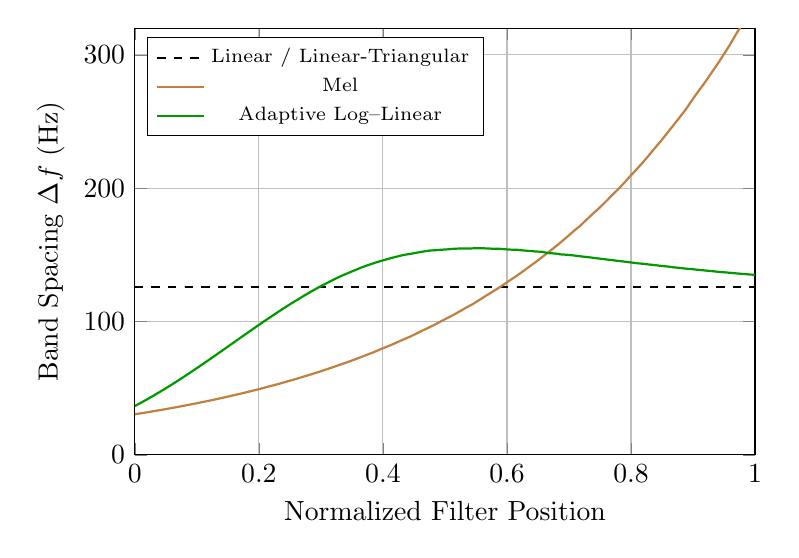
\begin{tikzpicture}
				\begin{axis}[
					width=0.78\textwidth,
					height=7cm,
					xlabel={Normalized Filter Position},
					ylabel={Band Spacing \(\Delta f\) (Hz)},
					xmin=0, xmax=1,
					ymin=0, ymax=320,
					grid=major,
					legend style={font=\scriptsize, at={(0.02,0.98)}, anchor=north west},
					samples=100
				]
					\def\fminA{80}
					\def\fmaxA{8000}
					\def\K{64}
					\def\breakPointA{1900}
					\def\alphaA{(\breakPointA - \fminA)/(\fmaxA - \fminA)}
					\addplot[black, thick, dashed, domain=0:1]
					{(\fmaxA-\fminA)/(\K-1)};
					\addlegendentry{Linear / Linear-Triangular}

					\addplot[brown, thick, domain=0:1]
					{700*(10^((2595*log10(1+\fminA/700) + (x + 1/(\K-1))*(2595*log10(1+\fmaxA/700)-2595*log10(1+\fminA/700)))/2595)-1)
					-700*(10^((2595*log10(1+\fminA/700) + x*(2595*log10(1+\fmaxA/700)-2595*log10(1+\fminA/700)))/2595)-1)};
					\addlegendentry{Mel}

					\addplot[green!60!black, thick, domain=0:1]
					{((1 - (1/(1+exp(-5*((x + 1/(\K-1))-\alphaA))))) * (\fminA * (\fmaxA/\fminA)^(x + 1/(\K-1))) +
					(1/(1+exp(-5*((x + 1/(\K-1))-\alphaA)))) * (\fminA + (x + 1/(\K-1))*(\fmaxA - \fminA)))
					-((1 - (1/(1+exp(-5*(x-\alphaA))))) * (\fminA * (\fmaxA/\fminA)^x) +
					(1/(1+exp(-5*(x-\alphaA)))) * (\fminA + x*(\fmaxA - \fminA)))};
					\addlegendentry{Adaptive Log--Linear}
				\end{axis}
			\end{tikzpicture}
			\caption[Effective spacing between adjacent frequency bands.]{Effective spacing between adjacent frequency bands across the filter axis. The horizontal axis is the normalized filter index, from the lowest-frequency filter (\(x=0\)) to the highest-frequency one (\(x=1\)); the vertical axis reports the gap in Hz between neighboring bands. Lower values therefore indicate denser spectral sampling and higher local frequency resolution. Linear and linear-triangular mappings keep this spacing constant, mel progressively widens it toward higher frequencies, and the adaptive log--linear front-end concentrates resolution in the low-frequency region before moving toward a more uniform allocation.}
			\label{fig:spectrogram_representation_comparison}
		\end{figure}

		Figure~\ref{fig:spectrogram_representation_comparison} should be read as a resolution-allocation plot rather than as a direct spectrogram image. A flat curve means that all filters are spaced uniformly in Hz. A rising curve means that adjacent filters become progressively farther apart, so high-frequency regions are represented more coarsely. The adaptive log--linear curve is informative because it stays below the mel curve over a substantial part of the low and mid spectrum, indicating that more filters are allocated where bird vocalizations often contain their most discriminative structure, while still avoiding the rigid perceptual prior imposed by a fully mel-scaled mapping.

	\begin{figure}[H]
		\centering
		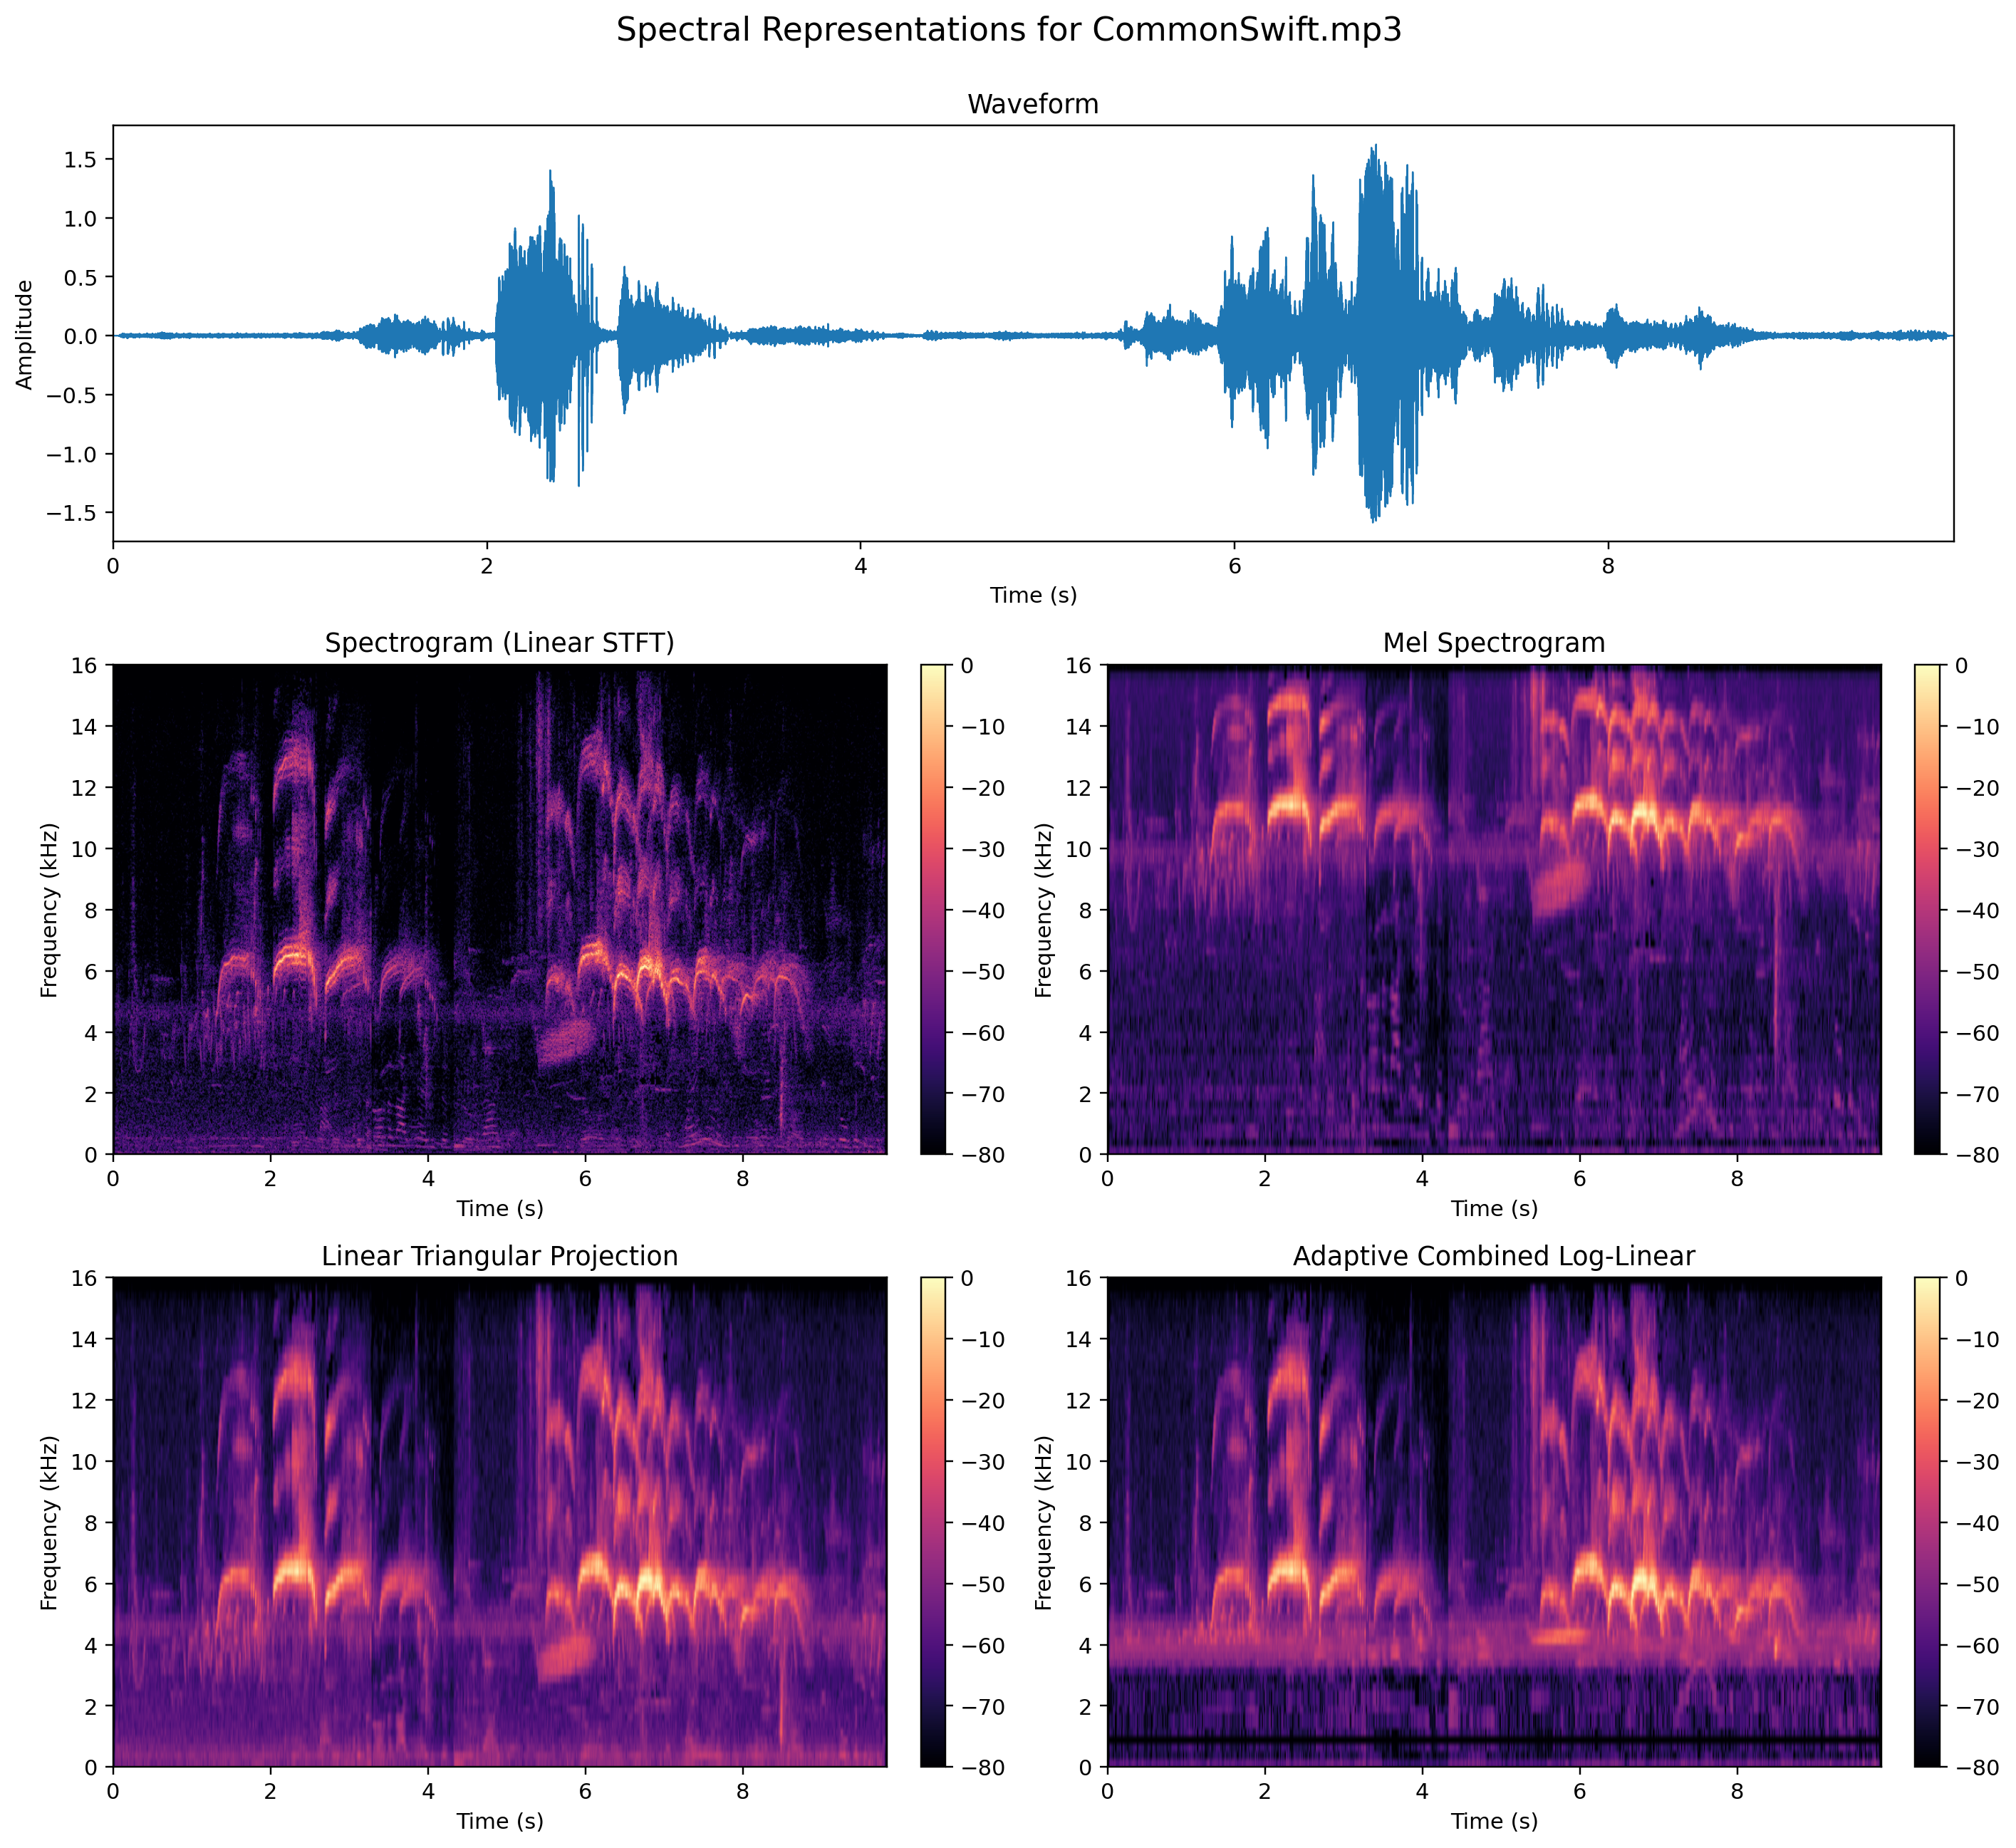
\includegraphics[width=0.95\textwidth]{images/generated/commonswift_representations/commonswift_representations_grid.png}
		\caption[Spectral-representation comparison on an \emph{Apus apus} recording.]{Example comparison of spectral representations computed on a \emph{Apus apus} recording. The figure reports the waveform together with four time--frequency views: linear STFT spectrogram, mel spectrogram, linear triangular projection, and adaptive combined log--linear projection. The comparison makes the representation trade-off visually explicit: the raw STFT preserves the highest spectral detail, mel compresses the frequency axis according to a perceptual prior, the linear triangular front-end preserves uniform frequency emphasis with reduced dimensionality, and the adaptive log--linear front-end concentrates resolution where the learned filter allocation is most informative.}
		\label{fig:commonswift_representation_grid}
	\end{figure}

		A compact expression of this mixed representation is
	\begin{equation}
		S_{\mathrm{combined}} = \alpha \odot S_{\log} + (1-\alpha)\odot S_{\mathrm{linear}},
	\end{equation}
	where \(\alpha\) is frequency-dependent and controlled by the learnable transition parameters. In the notation of the previous subsection, \(\alpha\) is implemented through the sigmoid gate \(S(x_i;b,w)\), so the model learns where log emphasis and linear emphasis should dominate.

	Across the tested configurations, this adaptive representation gives the best accuracy--efficiency balance. In dedicated nine-class distilled runs, it reaches high-80s test accuracy, with best observed performance around \(88.37\%\), while remaining compatible with compact edge-oriented models.

	\subsubsection{Fixed, Semi-Learnable, and Fully Learnable Filter Banks}
	A fixed filterbank has zero trainable front-end parameters and therefore minimal optimization overhead, but it cannot adapt its spectral allocation to the actual class set. A fully learnable filterbank removes this structural prior and learns each coefficient independently. If the front-end uses \(N\) filters and \(K\) frequency bins, the filter matrix \(F\in\mathrm{R}^{N\times K}\) is fully trainable and produces
	\begin{equation}
		Z_m(t)=\sum_k F_{m,k}\,|X_t(k)|.
	\end{equation}
	With \(N=64\) and \(K=513\), this introduces \(64\times513=32{,}832\) trainable front-end parameters.

	The semi-learnable alternative keeps the triangular structure and optimizes only the global transition parameters \(b\) and \(w\). The difference is substantial: \(2\) trainable front-end parameters versus \(32{,}832\). In the controlled \(8(+1)\) comparison reported later, the fully learnable model has \(70{,}442\) total parameters, compared with \(57{,}546\) for the semi-learnable configuration. The semi-learnable design therefore retains a clearly lower footprint while preserving adaptation capacity and interpretability.

	A fully learnable front-end must optimize thousands of unconstrained coefficients, which increases training variance and can overfit dataset-specific artifacts. The combined log--linear front-end instead constrains the hypothesis space with a physically meaningful parameterization and learns only where the log-to-linear transition should occur and how smooth that transition should be. This usually improves optimization stability, keeps the learned representation interpretable, and reduces computational and engineering cost across the full training cycle.

	\subsubsection{Why It Works in Practice}
	The key effect is that the filterbank learns to stabilize around values that improve separability for the species subset currently being learned. This behavior is especially evident in monoclass or very narrow-subset settings, where the learned breakpoint can move markedly toward the spectral region that carries the most discriminative cues for that specific species. By contrast, when the task spans many acoustically diverse species, the learned mapping tends to converge toward a more linear allocation. If different species occupy different niches of the acoustic space, the most robust global compromise is to preserve a broader and more uniform spectral coverage. When the dataset requires fine discrimination in low-frequency content, the learned transition tends to move toward values that preserve resolution in that region. When the relevant information is concentrated elsewhere, the transition shifts accordingly. In other words, the front-end learns where spectral detail is most useful for the task, without losing the inductive bias of triangular filters.

	Mel scaling remains a standard baseline because it encodes a perceptually motivated frequency warping derived from human auditory sensitivity, and for this reason it has long been treated as a reasonable default in audio classification pipelines. However, this inductive bias is not inherently optimal for bird vocalizations. Avian acoustic signals are organized according to species-specific production and ecological constraints rather than human perceptual criteria, so a representation calibrated on human hearing can be suboptimal for fine-grained bioacoustic discrimination. The semi-learnable front-end addresses this limitation by preserving the stability and interpretability of a structured filterbank while introducing a small number of trainable degrees of freedom. This allows the model to adapt spectral allocation to the statistics of the target bird community without incurring the instability and parameter cost of a fully unconstrained representation.

	Empirically, this behavior appears as convergence of breakpoint and transition width to stable values that differ across species subsets. In representative runs initialized with a breakpoint around \(4\,\mathrm{kHz}\), the learned transition often moves toward lower values (approximately \(1.9\,\mathrm{kHz}\)), indicating stronger logarithmic emphasis in the low-frequency region where many discriminative bird cues are concentrated. The best-performing subset-level models show that this adaptive mechanism generally outperforms both fixed mel-style mappings and unconstrained fully learnable filter matrices in the same parameter range, indicating that structure plus limited adaptability is a strong trade-off.

	\subsection{Model Architecture}
	\begin{figure}[H]
		\centering
		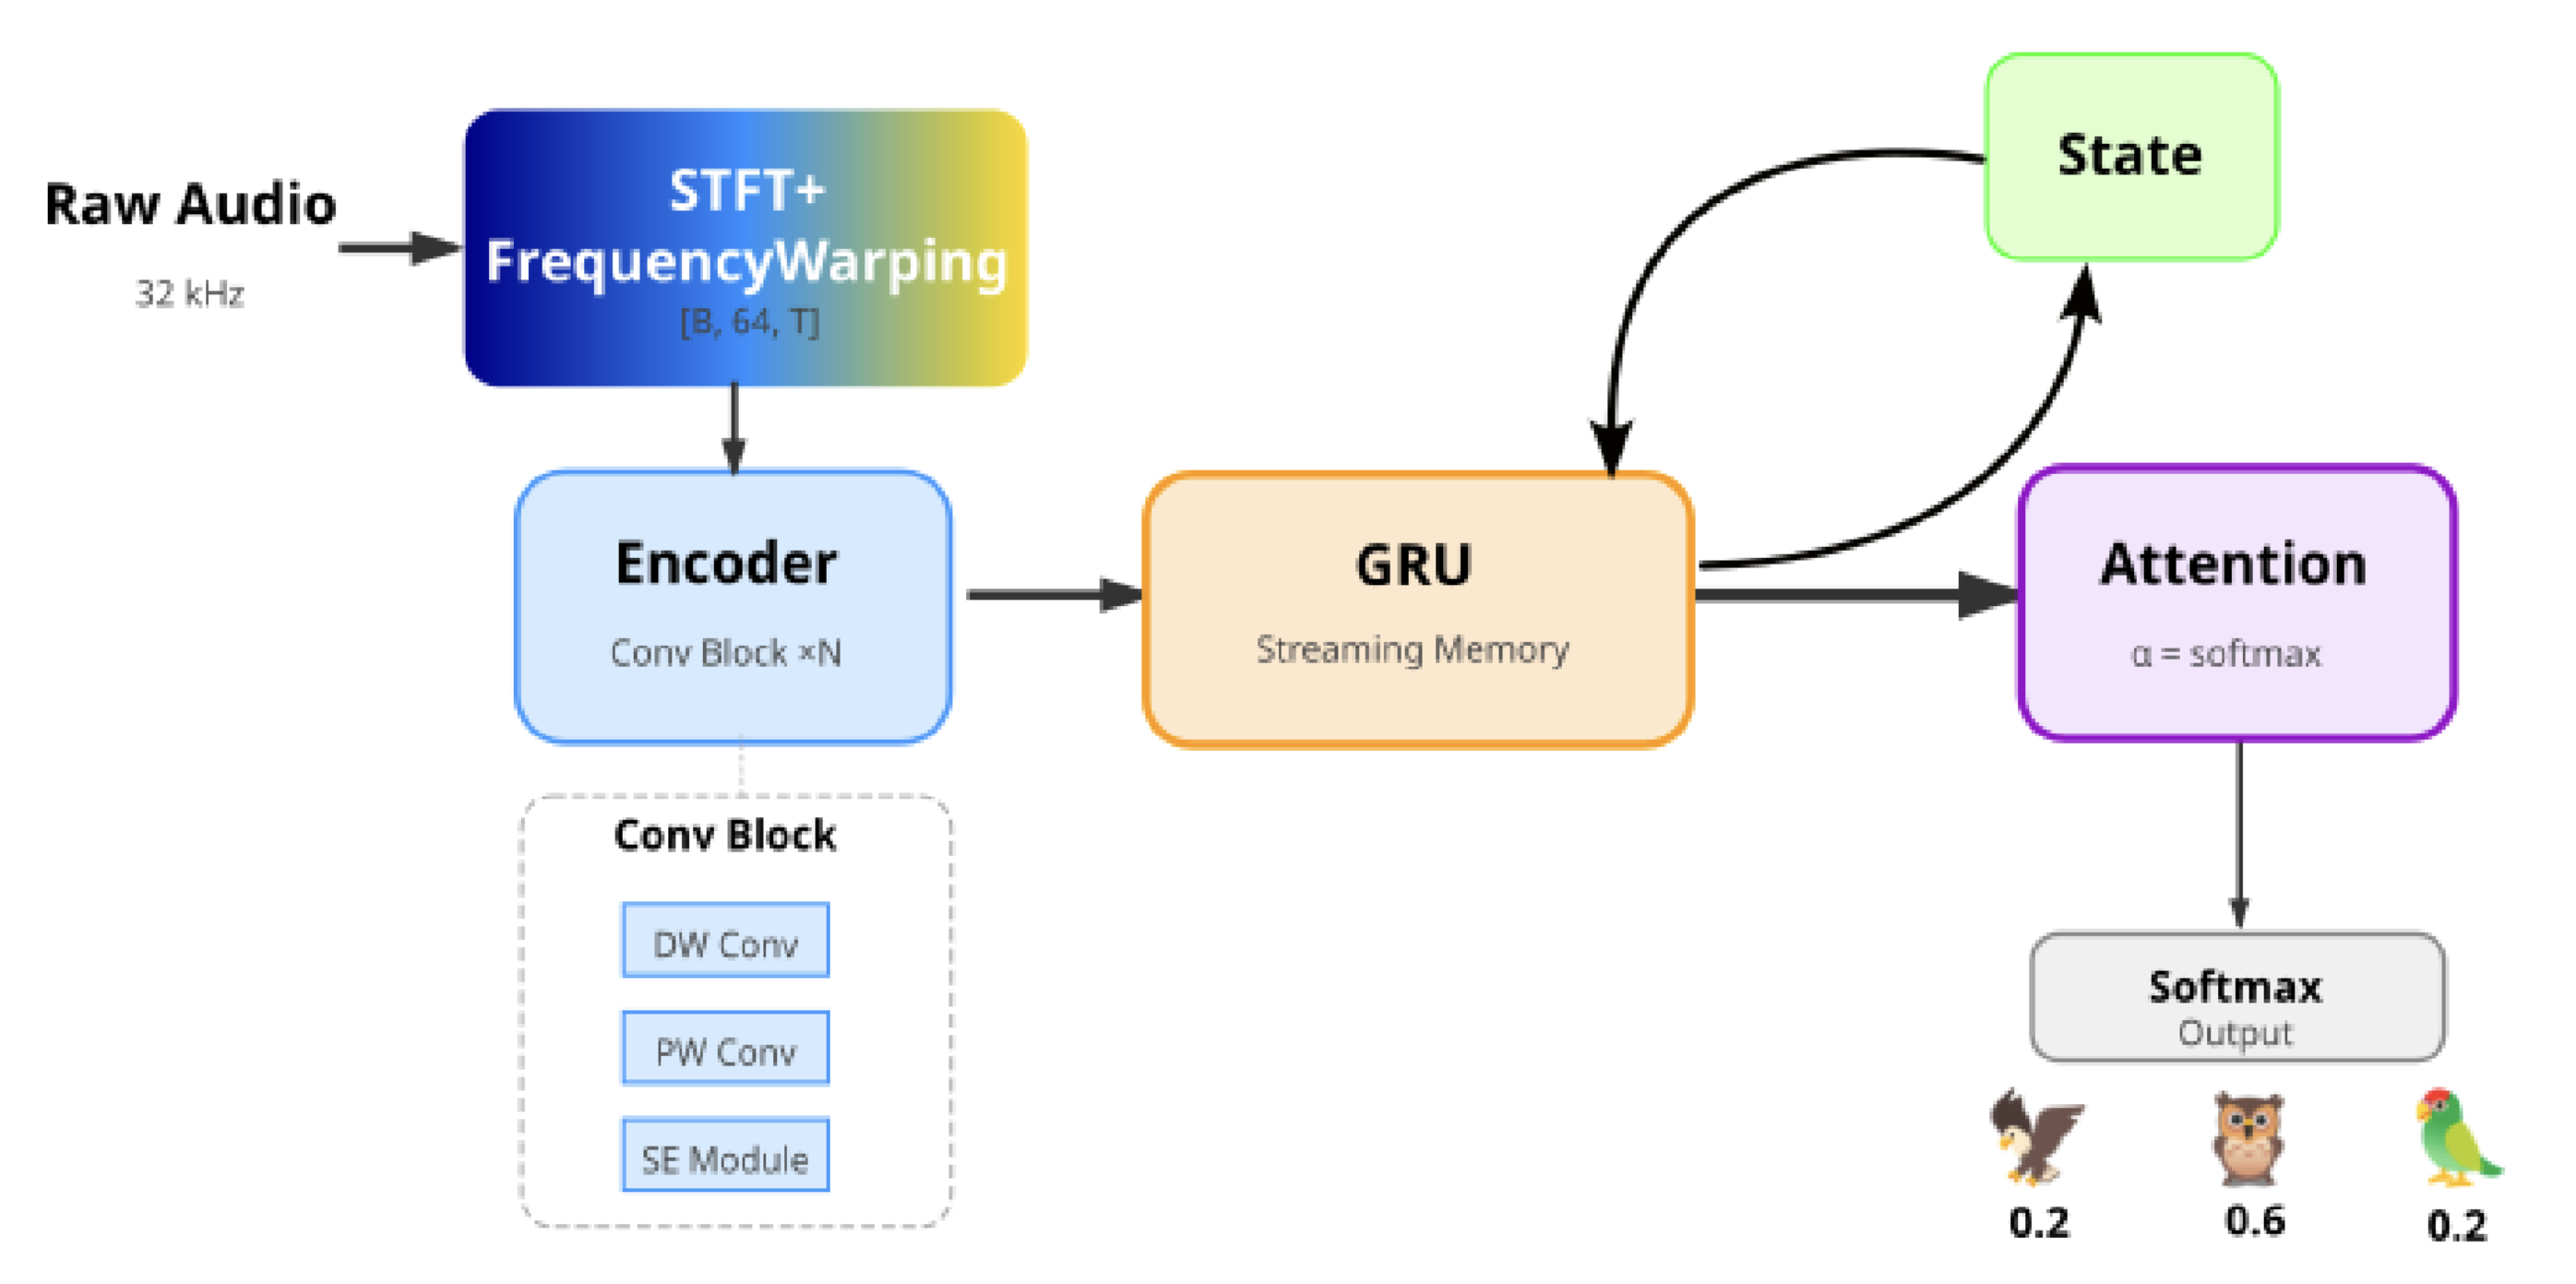
\includegraphics[width=0.96\textwidth]{images/model_architecture.png}
		\caption{Overall architecture of WrenNet from spectral input to classification output.}
		\label{fig:model_architecture_pipeline}
	\end{figure}

	\subsubsection{Waveform and Spectral Front-End}
	In \emph{WrenNet}, the first processing stage is the spectral front-end.

	In implementation, the model first enforces a consistent input layout and then applies one of several spectrogram families. In the strongest configuration used in the experiments, the front-end is the semi-learnable combined log--linear module. The waveform is transformed into an STFT magnitude representation, projected through the adaptive triangular filterbank, converted to decibel scale, and finally normalized per clip. The full mathematical definition of this stage is reported in Section~\ref{sec:semi_learnable_filter_design}. At architectural level, the key point is that this block outputs a stable fixed-shape tensor for the temporal encoder.

	\subsubsection{Convolutional Backbone}
	A Convolutional Neural Network learns local detectors that slide over the input and respond to recurring short patterns \cite{lecun1998cnn}. In bioacoustics, these patterns are not visual edges but spectral-time fragments such as onsets, narrow-band harmonics, chirp sweeps, and repeated modulation motifs. Weight sharing makes this mechanism efficient because the same detector can fire at any time location.

	The encoder in this model follows a compact temporal convolutional design, with low-power principles aligned with efficient audio backbones reported in the literature \cite{matchboxnet2020,phinets2022}. The core unit is a causal depthwise-separable convolutional block. Causality is implemented by left-only temporal padding \(P=d(k-1)\), where \(d\) is dilation and \(k\) is kernel size, so no future frame is used to compute the current output. This is relevant for streaming-oriented deployment and for preserving a strict temporal interpretation of features.

		Inside each block, the transformation is organized into four stages: expansion \(1\times1\), depthwise temporal convolution, squeeze-and-excitation recalibration, and projection \(1\times1\). In compact notation, for channel \(c\),
	\begin{equation}
		u_c = k_c * x_c, \qquad
		v_o = \sum_c p_{o,c}\,u_c,
	\end{equation}
	where \(k_c\) are depthwise temporal kernels and \(p_{o,c}\) are pointwise mixing coefficients. Channel recalibration is performed by a sigmoid gate computed from global pooled context:
	\begin{equation}
		s=\sigma\!\left(W_2\,\delta(W_1\,\mathrm{GAP}(u))\right), \qquad \hat{u}_c(t)=s_c\,u_c(t).
	\end{equation}
	This mechanism increases response for informative channels and suppresses less useful ones.

		\begin{sloppypar}
		At network level, the instantiated temporal convolutional backbone is composed of an initial block, three major temporal blocks, and two final blocks. Each major block contains two sub-blocks and residual pathways. Dilation patterns are chosen to expand the receptive field without temporal downsampling in the compact setting. The architecture therefore combines local precision and broader temporal context while preserving frame resolution for the recurrent stage.
		\end{sloppypar}

	\subsubsection{GRU: Temporal Memory Beyond Local Convolutions}
	Convolutions extract strong local patterns, but bird vocalizations also require temporal memory across longer windows, especially when discriminative cues depend on rhythm, repetition spacing, or call evolution. The recurrent stage is a unidirectional GRU \cite{cho2014gru}. This choice is a practical compromise between a basic recurrent unit and a full LSTM. A simple RNN is lighter, but its single-state update is more fragile when information must be retained across many frames. An LSTM offers stronger memory control, but it does so with a larger internal state, additional gates, and more partial activations that must be computed and stored during inference. For a low-power bioacoustic model, the GRU keeps gating and stable temporal memory while avoiding part of the state-management overhead of an LSTM. Given feature vector \(x_t\) and previous state \(h_{t-1}\), it computes
	\begin{equation}
		z_t=\sigma(W_z x_t + U_z h_{t-1} + b_z),
	\end{equation}
	\begin{equation}
		r_t=\sigma(W_r x_t + U_r h_{t-1} + b_r),
	\end{equation}
	\begin{equation}
		\tilde{h}_t=\tanh(W_h x_t + U_h(r_t \odot h_{t-1}) + b_h),
	\end{equation}
	\begin{equation}
		h_t=(1-z_t)\odot h_{t-1} + z_t \odot \tilde{h}_t.
	\end{equation}
	The update gate \(z_t\) controls how much new evidence replaces memory, while \(r_t\) controls how strongly the past contributes to the candidate state. Compared with an LSTM, the GRU does not maintain a separate cell state and therefore requires fewer gating operations and less state to carry across time, which is advantageous in constrained inference settings. Compared with a plain RNN, it still provides explicit mechanisms to preserve or overwrite temporal evidence in a controlled way. In the compact student configuration, the GRU receives \(32\)-dimensional frame features from the convolutional backbone and produces \(64\)-dimensional temporal states. A subsequent linear projection maintains the \(64\)-dimensional latent space and regularizes the transition toward attention pooling.

	\subsubsection{Attention Pooling and Classifier}
	After recurrent processing, the network has a sequence \(\{h_t\}_{t=1}^{T}\) of temporal states. Not every frame is equally informative, so the model applies learned temporal weighting. The implemented attention is deliberately lightweight: one linear scorer maps each \(h_t\in\mathrm{R}^{64}\) to a scalar logit, softmax normalizes these logits across time, and the context vector is formed by weighted summation:
	\begin{equation}
		e_t = w^\top h_t + b, \qquad
		\alpha_t = \frac{\exp(e_t)}{\sum_{j=1}^{T}\exp(e_j)},
	\end{equation}
	\begin{equation}
		c = \sum_{t=1}^{T}\alpha_t h_t.
	\end{equation}
	The classifier is a final linear layer:
	\begin{equation}
		o = W_c c + b_c, \qquad
		p(c \mid x)=\frac{\exp(o_c)}{\sum_j \exp(o_j)}.
	\end{equation}
	Operationally, this stage compresses a long temporal sequence into one discriminative embedding while preserving frame importance through \(\alpha_t\). This is one of the reasons the architecture remains compact without discarding temporal selectivity.

	\subsubsection{Layer-Wise Tensor Flow in WrenNet}
	Let \(B\) be batch size, \(L\) waveform length in samples, \(F\) number of front-end filters, \(F_c\) number of CNN output channels, \(H_d\) recurrent hidden size, \(T\) number of time frames after STFT, and \(C\) number of classes. For a \(3\)-second clip at \(32\)~kHz, \(L=96{,}000\).

	The forward path is
	\begin{equation}
		\begin{array}{rcll}
			X &\in& \mathrm{R}^{B\times L} & \mbox{(raw waveform)}\\
			S &=& \Phi_{\mathrm{FE}}(X) \in \mathrm{R}^{B\times F\times T} & \mbox{(STFT + filterbank)}\\
			H &=& \Phi_{\mathrm{CNN}}(S) \in \mathrm{R}^{B\times F_c\times T} & \mbox{(convolutional backbone)}\\
			R &=& \Phi_{\mathrm{GRU}}\!\left(H^{\top}\right) \in \mathrm{R}^{B\times T\times H_d} & \mbox{(temporal states)}\\
			c &=& \Phi_{\mathrm{att}}(R) \in \mathrm{R}^{B\times H_d} & \mbox{(attention context)}\\
			o &=& \Phi_{\mathrm{cls}}(c) \in \mathrm{R}^{B\times C} & \mbox{(logits)}\\
			p &=& \mathrm{softmax}(o) \in \mathrm{R}^{B\times C} & \mbox{(probabilities).}
		\end{array}
	\end{equation}

	Here \(H^{\top}\) indicates the channel-time permutation needed by the GRU input format, from \(B\times F_c\times T\) to \(B\times T\times F_c\). In other words, each symbol in the path represents one tensor after one block: \(X\) raw audio, \(S\) spectral representation, \(H\) convolutional features, \(R\) recurrent sequence, \(c\) pooled embedding, \(o\) class logits, and \(p\) class probabilities.

	In the compact configuration, \(F=64\), \(F_c=32\), \(H_d=64\). This decomposition clarifies that only the final classifier depends directly on \(C\), while front-end, CNN, recurrent, and attention layers remain class-agnostic and therefore reusable across class-set variants.

	\subsubsection{Concrete Instantiation Used in the Main Experiments}
	The concrete student used in the main distilled experiments is built around the combined log--linear front-end with trainable \(b\) and \(w\), \(64\) spectral filters, a temporal convolutional backbone with \(32\) base channels, a single-direction GRU with hidden size \(64\), scalar temporal attention, and a linear classification head. This design keeps representational capacity where it most affects difficult bioacoustic boundaries, while avoiding heavy recurrent stacks or high-channel convolutional expansions.

	Operationally, experiment families differ in STFT resolution according to target trade-offs. Subset-focused runs commonly use \(n_{\mathrm{fft}}=1024\), \(\mathrm{hop}=320\) to preserve fine spectral detail. In the main distillation protocol, a lighter setting with \(n_{\mathrm{fft}}=512\) and \(\mathrm{hop}=320\) is used together with 64 filters, initial breakpoint \(b_0=8000\)~Hz, and initial transition width \(w_0=200\). Across these settings, the compact architecture remains in the low-\(10^4\) parameter regime and, in representative runs, around \(5.3\times10^4\) parameters, with class count affecting mainly the last linear layer.

	A central empirical observation is that the learnable front-end parameters converge to stable values during training and adapt with task conditions. For example, runs initialized around \(4\)~kHz show learned breakpoints moving to lower frequencies with moderate transition widths, indicating that the model concentrates spectral resolution where the current species subset is most discriminative. This is consistent with the central hypothesis that semi-learnable filtering improves the representation-quality to complexity ratio in edge-oriented bird classification.

	\subsubsection{Parameter Choices and Scaling with Class Cardinality}
	Parameter selection follows a strict efficiency-first criterion. The compact operating point uses \(F=64\) front-end filters, \(F_c=32\) convolutional channels after the temporal convolutional backbone, and \(H_d=64\) recurrent hidden units. These values are large enough to preserve discriminative temporal-spectral structure in difficult species groups, but small enough to keep memory pressure and inference cost compatible with on-device execution.

	The main architectural scaling law is straightforward. If \(C\) is the number of classes, only the final classifier scales directly with \(C\), with
	\begin{equation}
		P_{\mathrm{cls}} = H_d \cdot C + C.
	\end{equation}
	All upstream blocks, including front-end, convolutional encoder, recurrent unit, and attention pooling, are class-agnostic and therefore reusable when the taxonomy changes.

	This decomposition explains why the same model family can be instantiated across subsets with different cardinality. Moving from small subsets to larger class inventories increases output-layer parameters and confusion complexity, while preserving most of the internal representation pipeline. In the reported experiments, compact configurations remain around the mid-\(10^4\) to low-\(10^5\) parameter range depending on class count and width multipliers, and larger variants increase absolute accuracy at the expected cost of higher memory and energy demand. The selected compact configuration is therefore a deliberate compromise: it preserves separability on hard classes while remaining viable under embedded deployment constraints.

	\subsubsection{Distillation in the Architecture Workflow}
	\label{sec:distillation_workflow}
	Distillation is a training-only technique in this work: it improves how \emph{WrenNet} is optimized, but it does not modify the deployed inference graph and therefore does not directly affect on-device inference time, memory footprint, or operator set. The implementation uses BirdNET as teacher and follows an offline-two-stage pipeline: teacher soft targets are generated first (confidence threshold \(0.05\)), then the student is optimized with focal distillation. In the main configuration, training uses \(\alpha=0.4\), \(T=3.0\), \(\gamma=4.0\), and adaptive distillation rate \(0.1\). The full mathematical definition of distillation and focal distillation losses is reported in Section~\ref{sec:training_objectives_losses}.

	\subsection{Training Objectives and Loss Functions}
	\label{sec:training_objectives_losses}
	\subsubsection{Cross-Entropy}
	Cross-entropy is the standard loss for multi-class classification. For one sample with one-hot target \(y\) and predicted probabilities \(p\), it is
	\begin{equation}
		\mathcal{L}_{\mathrm{CE}} = -\sum_{c=1}^{C} y_c \log p_c.
	\end{equation}
	Because only the true class has \(y_c=1\), this reduces to \(-\log p_{y^\ast}\). Minimizing cross-entropy increases probability assigned to the correct class.

	\subsubsection{Focal Loss}
	Focal loss modifies cross-entropy to focus learning on hard examples \cite{lin2017focal}:
	\begin{equation}
		\mathcal{L}_{\mathrm{focal}} = -\alpha_{y^\ast}(1-p_{y^\ast})^\gamma \log p_{y^\ast}.
	\end{equation}
	Equivalently, with \(p_t\) denoting the model probability assigned to the true class, one writes
	\begin{equation}
		\mathcal{L}_{\mathrm{focal}} = -\alpha_t(1-p_t)^\gamma \log p_t.
	\end{equation}
	The modulating factor \((1-p_t)^\gamma\) is close to zero for easy, high-confidence samples and close to one for difficult, low-confidence samples. As a result, easy examples contribute much less to gradient updates, while hard examples remain influential for longer during training. The class-dependent weight \(\alpha_t\) addresses class-frequency imbalance by scaling minority-class contributions upward and majority-class contributions downward.

	In this application, focal loss directly addresses the training dynamics of bird-sound classification. Species difficulty is uneven, recordings include strong background variability, and the negative class must be separated from many non-bird acoustic patterns. In these conditions, plain cross-entropy is quickly dominated by abundant easy examples. Focal loss keeps meaningful gradient pressure on ambiguous species boundaries and low-SNR segments, which are the cases that matter most for field performance.
	In the main training protocol, focal loss is instantiated with \(\gamma=4.0\) and automatic class weighting, so hard and minority cases continue to contribute to parameter updates even when easy examples dominate the batch.

	\subsubsection{Distillation Loss}
	Knowledge distillation transfers information from a stronger teacher model to a compact student \cite{hinton2015distilling}. The student is trained with two targets: hard labels from the dataset and soft targets from the teacher. Let \(z_s\) and \(z_t\) be student and teacher logits. With temperature \(T\), define
	\begin{equation}
		q_s^{(T)}(c)=\frac{\exp(z_{s,c}/T)}{\sum_j \exp(z_{s,j}/T)}, \qquad
		q_t^{(T)}(c)=\frac{\exp(z_{t,c}/T)}{\sum_j \exp(z_{t,j}/T)}.
	\end{equation}
	The soft term uses temperature-scaled KL divergence:
	\begin{equation}
		\mathcal{L}_{\mathrm{KD}} = T^2 \sum_{c=1}^{C} q_t^{(T)}(c)\log \frac{q_t^{(T)}(c)}{q_s^{(T)}(c)}.
	\end{equation}
	The total distillation objective is
	\begin{equation}
		\mathcal{L}_{\mathrm{distill}} = (1-\lambda)\mathcal{L}_{\mathrm{CE}} + \lambda \mathcal{L}_{\mathrm{KD}}.
	\end{equation}
	In this expression, the first term is often called the \emph{hard CE term}, and the second term is the \emph{temperature-scaled KL term}. Hard CE enforces fidelity to ground-truth labels. The KL term transfers teacher uncertainty structure, which contains information about class similarities.

	In the main distilled configuration used in this thesis, this objective is written as \(\mathcal{L}_{\mathrm{distill}}=(1-\alpha)\mathcal{L}_{\mathrm{hard}}+\alpha T^2\mathcal{L}_{\mathrm{soft}}\), with \(\alpha=0.4\) and \(T=3.0\). In this parameterization, \(\alpha\) is the soft-target weight; therefore, the hard branch has weight \(0.6\) and the soft branch has weight \(0.4\).

	\subsubsection{Focal Distillation}
	Focal distillation replaces the hard CE term with focal loss:
	\begin{equation}
		\mathcal{L}_{\mathrm{focal\_distill}} = (1-\lambda)\mathcal{L}_{\mathrm{focal}} + \lambda \mathcal{L}_{\mathrm{KD}}.
	\end{equation}
	In expanded form, the hard branch is
	\begin{equation}
		\mathcal{L}_{\mathrm{focal\_hard}} = -\alpha_t(1-p_t)^\gamma \log p_t,
	\end{equation}
	and the soft branch is
	\begin{equation}
		\mathcal{L}_{\mathrm{KL\_soft}} = T^2\sum_{c=1}^{C} q_t^{(T)}(c)\log\frac{q_t^{(T)}(c)}{q_s^{(T)}(c)}.
	\end{equation}
	The complete objective can therefore be read as
	\begin{equation}
		\mathcal{L}_{\mathrm{focal\_distill}} = (1-\lambda)\mathcal{L}_{\mathrm{focal\_hard}} + \lambda\mathcal{L}_{\mathrm{KL\_soft}}.
	\end{equation}
	At implementation level, training may use mixed batches that contain both distillation samples (with teacher soft targets) and supervised-only samples (without soft targets). Let \(\mathcal{D}\) be indices with soft targets and \(\mathcal{S}\) indices without soft targets. The optimized batch objective is
	\begin{equation}
		\mathcal{L}_{\mathrm{batch}}
		= 1_{|\mathcal{D}|>0}\,\mathcal{L}_{\mathrm{focal\_distill}}^{(\mathcal{D})}
		+ 1_{|\mathcal{S}|>0}\,\mathcal{L}_{\mathrm{sup}}^{(\mathcal{S})},
	\end{equation}
	where \(\mathcal{L}_{\mathrm{sup}}\) is the supervised classification loss configured for non-distilled samples (focal loss in the main setup). With focal distillation enabled, \(\lambda=\alpha\), so in the main protocol \(\alpha=0.4\), \(T=3.0\), \(\gamma=4.0\), and adaptive distillation rate \(0.1\).
	This objective is particularly suitable when class imbalance and class difficulty coexist. The focal hard term preserves learning pressure on hard or minority examples; the KL soft term injects teacher-level structure over confusable classes. In relation to the rest of the pipeline, focal distillation is the optimization layer that operationalizes all earlier design choices: species-focused dataset construction, realistic augmentation, semi-learnable spectral emphasis, and compact temporal modeling. The empirical effect is coherent with this role, with stronger robustness on difficult species and stable high recall for the no-bird class while maintaining edge-compatible model size.

	\subsection{Implementation Quality and Reproducibility}
	The implementation was structured to separate data processing, model definition, loss construction, and experiment orchestration. This modular design supports reproducibility because each experimental run can be traced back to explicit hyperparameters, data configuration, and final metrics. It also supports extension: new front-ends, alternative losses, or additional species subsets can be introduced without rewriting the full training pipeline. This is essential because the project can easily become a reusable research framework for low-power bioacoustic classification.

		From a training-pipeline viewpoint, throughput is maintained through a resource-aware loading strategy. Small datasets can be preloaded to minimize latency, whereas larger corpora are processed on demand to bound memory footprint. Parallel data workers and pinned host memory are used in accelerator-based training to reduce pipeline stalls between input preparation and model execution.

		\begin{sloppypar}
		Memory stability is reinforced by controlling intermediate allocations in augmentation and feature extraction, and by reusing precomputed artifacts when available. In particular, pooled metadata for empty segments and optional caching of frequently accessed preprocessed inputs reduce repeated signal-processing overhead across epochs without weakening split isolation.
		\end{sloppypar}

	Experiment management is configuration-driven, with hierarchical settings that define defaults and controlled overrides for sampling ratios, augmentation behavior, front-end parameters, loss weighting, and optimization policies. This structure enables strict reproducibility and consistent run-to-run comparison because each run corresponds to an explicit, versioned parameter state rather than ad hoc script modifications.

	\subsection{Experimental Setup}
	\subsubsection{Experimental Protocol}
	This section explains how experiments are executed and compared. The intent is methodological transparency: each result in the following results subsections must be traceable to a clear training, validation, and test procedure.

	All experiments use the same data-governance principles described earlier in this chapter: fixed split policy, leakage control between training and evaluation, and deterministic seeds for reproducible partitioning. The acquisition and preprocessing chain starts from 150,645 downloaded recordings and produces 150,557 validated clips of 3 seconds at 32~kHz, with identical segmentation policy across training, validation, and test.

	The distillation setup used in experiments follows the same configuration defined in Section~\ref{sec:distillation_workflow} and formalized in Section~\ref{sec:training_objectives_losses}. In this section, those settings are applied unchanged to keep all runs directly comparable.

	Optimization is based on AdamW with learning rate \(10^{-3}\), weight decay \(0.01\), batch size \(64\), and cosine annealing over \(150\) epochs. Early stopping uses patience \(35\). Filter adaptation receives dedicated learning-rate amplification, with multiplier \(15\times\) for breakpoint updates and \(5\times\) for transition-width updates. The alternating strategy applies \(5\) initial epochs of joint optimization, then cycles of \(5\) epochs focused on main-network updates and \(1\) epoch focused on filter updates, and closes with \(20\) final joint-refinement epochs.

	Model selection is performed on validation metrics, while final reporting is reserved for the held-out test split. Reported classification metrics include test accuracy and weighted \(F1\), together with class-aware interpretation in the discussion chapter. For teacher--student fairness analysis, direct Student/BirdNET comparisons are reported on the shared species classes, excluding the explicit ``no bird'' class that is unique to the student formulation.

	\subsubsection{Experiments}
	The main experimental campaign is structured around a small set of directly comparable scenarios. The first scenario evaluates front-end design on controlled subsets, including semi-learnable and fully learnable variants under matched conditions. The second scenario evaluates the compact architecture on easy and hard subsets to expose sensitivity to class confusability. The third scenario scales the task to the full species pool, including comparison between compact and larger architectures. The fourth scenario evaluates deployment behavior on edge-relevant hardware for the same model family.

	These scenarios correspond exactly to the results discussed below in this chapter. No additional experimental families are required for methodological coherence: the core contribution is already supported by front-end comparison, subset-difficulty analysis, full-scale classification evaluation, and device-level efficiency measurements.

	\subsection{Results}
	\subsubsection{Classification Results}
	The classification results confirm that the semi-learnable front-end provides the strongest accuracy-efficiency balance in the tested setup. On the \(8(+1)\) controlled subset, the semi-learnable variant outperforms the fully learnable alternative while remaining lighter in effective complexity. The easy subset yields the highest scores, while the hard subset produces a substantial drop, confirming that inter-species acoustic similarity remains the dominant challenge.

	For a cleaner comparison, classification quality and deployment efficiency are reported in separate tables. Table~\ref{tab:extended_results} summarizes recognition performance across model configurations and class scales, while Tables~\ref{tab:energy_benchmark} and \ref{tab:energy_relative_summary} summarize hardware-level latency, power, and energy behavior.

		These results clarify the practical positioning of the proposed system. BirdNET remains a strong globally scoped bird recognition reference. The deployment comparison shows that the low-power configuration operates at substantially lower energy cost per decision in continuous monitoring mode, reaching \(36.2\times\) in the reported benchmark setting.

	\begin{table}[H]
		\centering
		\scriptsize
		\renewcommand{\arraystretch}{1.15}
		\setlength{\tabcolsep}{6pt}
		\caption{Representative classification results across configurations.}
		\label{tab:extended_results}
		\begin{tabular}{|l|c|c|c|c|}
			\hline
			Configuration & Classes & Parameters & Test Acc (\%) & Test \(F1_w\) (\%) \\
			\hline
			Semi-learnable subset & 8(+1) & 57,546 & 87.22 & 87.25 \\
			\hline
			Fully learnable subset & 8(+1) & 70,442 & 83.83 & 83.84 \\
			\hline
			Easy species subset & 8(+1) & 57,546 & 90.76 & 90.90 \\
			\hline
			Hard species subset & 13(+1) & 57,546 & 77.47 & 77.97 \\
			\hline
			Full dataset compact model & 70(+1) & 57,546 & 66.51 & 67.49 \\
			\hline
			Full dataset larger model & 70(+1) & 136,906 & 70.14 & 70.81 \\
			\hline
		\end{tabular}
	\end{table}

	For consistency, the parameter count used in the comparative discussion is the measured one from the controlled \(8(+1)\) experiment, reported in Table~\ref{tab:semi_vs_fully_complexity}. In that setting, the fully learnable front-end model has \(70{,}442\) parameters, while the semi-learnable counterpart has \(57{,}546\).

	The complete experimental summary is easier to read when separated into thematic groups: core comparative runs, subset-specialized runs, focused case studies, and direct Student/BirdNET comparison for the focused scenarios. Tables~\ref{tab:full_experiment_summary_core}, \ref{tab:full_experiment_summary_subsets}, \ref{tab:full_experiment_summary_focused_metrics}, and \ref{tab:full_experiment_summary_focused_student_birdnet} therefore replace the previous single compressed summary table.

	\begin{table}[H]
		\centering
		\scriptsize
		\renewcommand{\arraystretch}{1.15}
		\setlength{\tabcolsep}{4pt}
		\caption{Adapted experimental summary for the full project: core comparative runs.}
		\label{tab:full_experiment_summary_core}
		\resizebox{\textwidth}{!}{%
		\begin{tabular}{|l|c|c|c|c|c|c|c|c|}
			\hline
			Experiment & Classes & Params & Epochs & Val Acc & Test Acc & F1$_w$ & Breakpoint & Trans. Width \\
			\hline
			Semi-learnable (subset baseline) & 8(+1) & 57k & 75 & 85.74 & 87.22 & 87.25 & 2741 & 67.79 \\
			\hline
			Fully learnable (subset) & 8(+1) & 70k & 75 & 84.26 & 83.83 & 83.84 & -- & -- \\
			\hline
			Full dataset (semi-learnable) & 70(+1) & 57k & 150 & 70.10 & 66.51 & 67.49 & 851 & 19.00 \\
			\hline
			Full dataset (larger model) & 70(+1) & 136k & 75 & 72.10 & 70.14 & 70.81 & 1390 & 33.86 \\
			\hline
		\end{tabular}
		}
	\end{table}

	\begin{table}[H]
		\centering
		\scriptsize
		\renewcommand{\arraystretch}{1.15}
		\setlength{\tabcolsep}{5pt}
		\caption{Adapted experimental summary for the full project: subset-specialized runs.}
		\label{tab:full_experiment_summary_subsets}
		\resizebox{\textwidth}{!}{%
		\begin{tabular}{|l|c|c|c|c|c|c|c|c|}
			\hline
			Experiment & Classes & Params & Epochs & Val Acc & Test Acc & F1$_w$ & Breakpoint & Trans. Width \\
			\hline
			Easy species subset & 8(+1) & 57k & 116 & 91.98 & 90.76 & 90.90 & 1.50 & 6.00 \\
			\hline
			Hard species subset & 13(+1) & 57k & 134 & 79.78 & 77.47 & 77.97 & 1224 & 27.42 \\
			\hline
			High-frequency subset & 5(+1) & 57k & 93 & 90.27 & 91.49 & 91.55 & 164 & 8.55 \\
			\hline
			Low-frequency subset & 4(+1) & 57k & 126 & 90.28 & 91.63 & 91.67 & 237 & 9.00 \\
			\hline
		\end{tabular}%
		}
	\end{table}

	\begin{table}[H]
		\centering
		\scriptsize
		\renewcommand{\arraystretch}{1.15}
		\setlength{\tabcolsep}{5pt}
		\caption{Adapted experimental summary for the full project: focused case studies.}
		\label{tab:full_experiment_summary_focused_metrics}
		\begin{tabular}{|l|c|c|c|c|c|c|}
			\hline
			Experiment & Classes & Epochs & Test Acc & F1$_w$ & Breakpoint & Trans. Width \\
			\hline
			Semi-learnable (subset baseline) & 8(+1) & 75 & 87.22 & 87.25 & 2741 & 67.79 \\
			\hline
			Easy species subset & 8(+1) & 116 & 90.76 & 90.90 & 1.50 & 6.00 \\
			\hline
			Hard species subset & 13(+1) & 134 & 77.47 & 77.97 & 1224 & 27.42 \\
			\hline
			Monoclass (\emph{Corvus corax}) & 1(+1) & 94 & 92.37 & 92.62 & 1955 & 51.79 \\
			\hline
			Monoclass (\emph{Upupa epops}) & 1(+1) & 45 & 94.71 & 94.67 & 5269 & 132.00 \\
			\hline
			Hard couple (\emph{Regulus} pair) & 2(+1) & 85 & 85.64 & 85.60 & 1221 & 28.34 \\
			\hline
			High-frequency subset & 5(+1) & 93 & 91.49 & 91.55 & 164 & 8.55 \\
			\hline
			Low-frequency subset & 4(+1) & 126 & 91.63 & 91.67 & 237 & 9.00 \\
			\hline
		\end{tabular}
	\end{table}

	\begin{table}[H]
		\centering
		\scriptsize
		\renewcommand{\arraystretch}{1.15}
		\setlength{\tabcolsep}{5pt}
		\caption[Student/BirdNET comparison on focused scenarios.]{Adapted experimental summary for the full project: Student/BirdNET comparison on focused scenarios.}
		\label{tab:full_experiment_summary_focused_student_birdnet}
		\begin{tabular}{|l|c|c|c|c|}
			\hline
			Experiment & Student Acc & BirdNET Acc & Student F1$_m$ & BirdNET F1$_m$ \\
			\hline
			Semi-learnable (subset baseline) & 86.33 & 88.19 & 85.76 & 86.93 \\
			\hline
			Easy species subset & 89.85 & 91.04 & 78.75 & 87.50 \\
			\hline
			Hard species subset & 73.90 & 82.86 & 68.00 & 79.30 \\
			\hline
			Monoclass (\emph{Corvus corax}) & 90.15 & 91.16 & 87.96 & 89.72 \\
			\hline
			Monoclass (\emph{Upupa epops}) & 86.35 & 89.45 & 85.52 & 88.97 \\
			\hline
			Hard couple (\emph{Regulus} pair) & 83.60 & 87.87 & 83.41 & 87.59 \\
			\hline
			High-frequency subset & 90.23 & 92.74 & 90.37 & 91.25 \\
			\hline
			Low-frequency subset & 85.15 & 91.01 & 85.72 & 89.44 \\
			\hline
		\end{tabular}
	\end{table}

	\subsubsection{Interpretation of the Semi-Learnable Front-End Behavior}
	A central observation across runs is that the learned front-end parameters do not drift randomly. They converge to stable regions that depend on the class subset and acoustic difficulty. This supports the intended role of the semi-learnable filterbank: preserve a strong spectral prior while still adapting frequency allocation to the discriminative needs of the current task.

	In many runs, the learned breakpoint moves away from initialization toward lower-frequency emphasis when this improves class separation for the active species set. This behavior is consistent with the acoustic structure of many bird calls, where relevant cues often concentrate in specific frequency bands rather than being uniformly distributed over the entire spectrum. The transition-width parameter complements this mechanism by controlling how sharp or smooth the log-linear change is. Together, these two parameters provide controlled flexibility with negligible model-size overhead.

	To make this interpretation auditable, Figure~\ref{fig:learned_frequency_mappings_16khz} reports the learned frequency mappings for representative runs. The plot compares reference mappings and learned mappings derived from the recorded \((b,w)\) values.

	\begin{figure}[H]
		\centering
		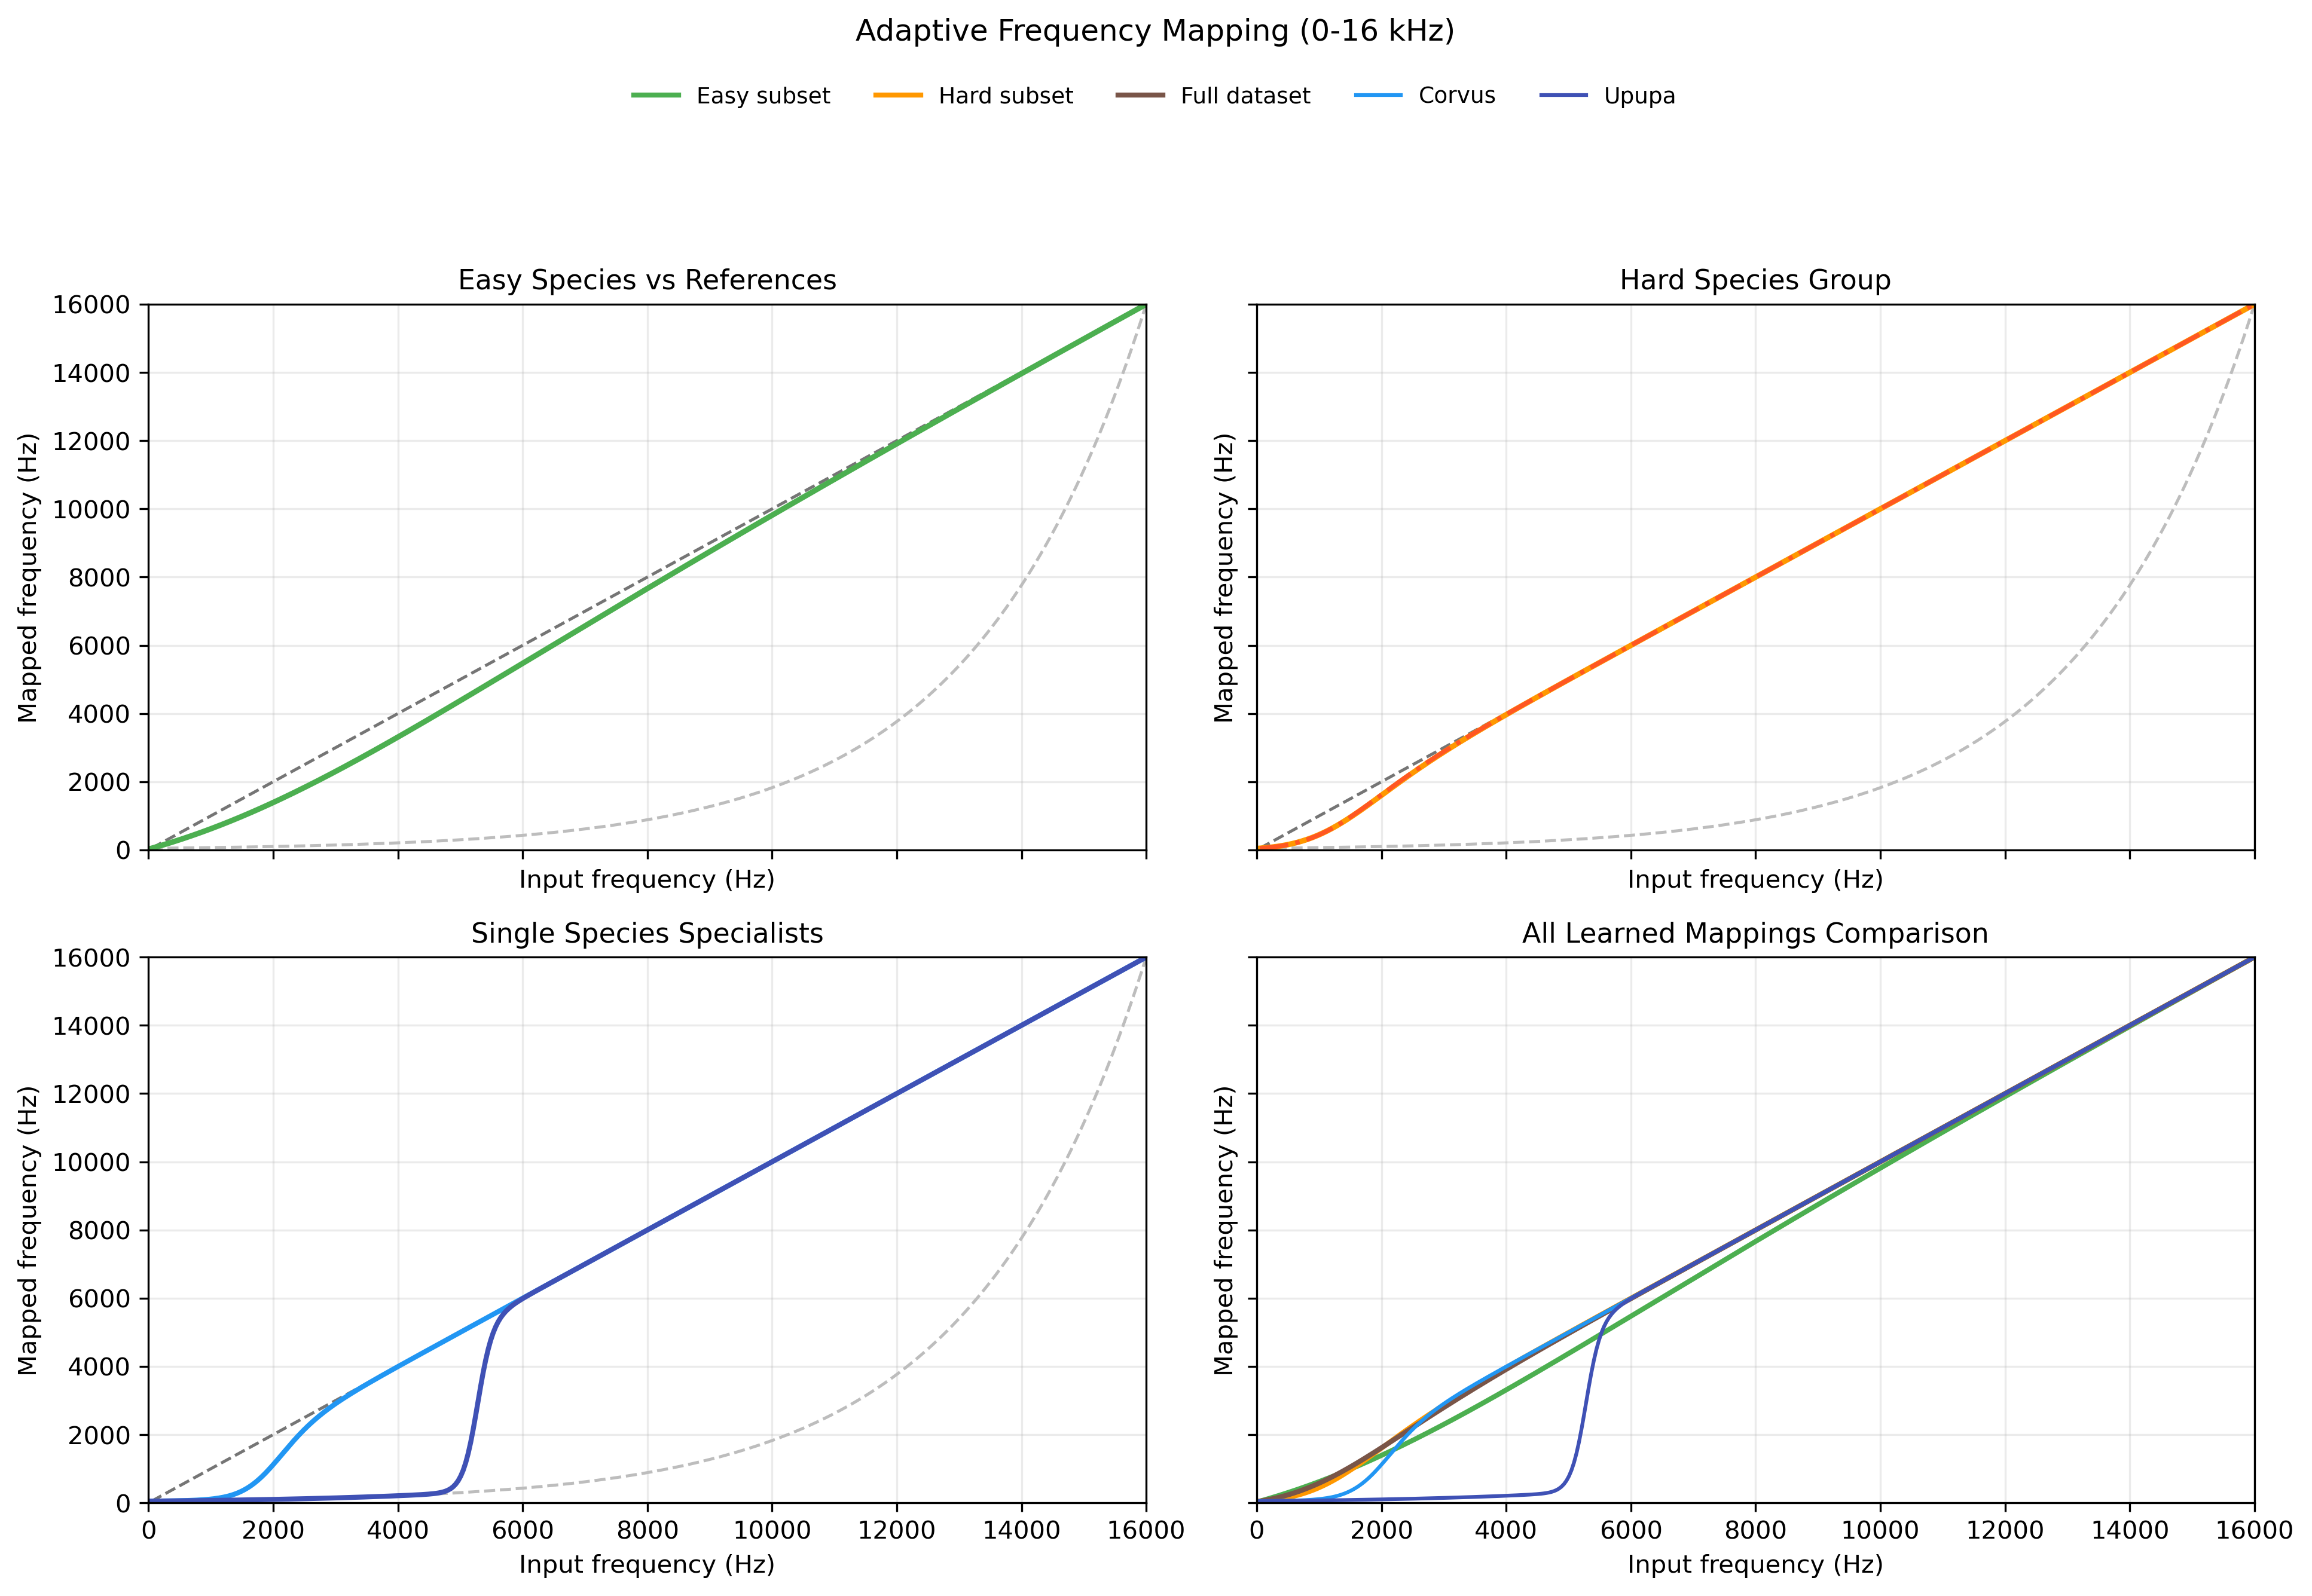
\includegraphics[width=0.96\textwidth]{images/learned_frequency_mappings_16khz.png}
		\caption[Learned frequency mappings from run-level parameters.]{Learned frequency mappings from run-level breakpoint and transition-width values (\(0\)--\(16\) kHz). Curves are generated with the adaptive mapping equations used by the proposed front-end.}
		\label{fig:learned_frequency_mappings_16khz}
	\end{figure}

	The figure supports three consistent observations. First, the easy subset (\(b\approx 1.5\), \(w\approx 6\)) remains close to a linear mapping across most of the band. Second, the hard subset (\(b\approx 1224\), \(w\approx 27.4\)) preserves stronger low-frequency emphasis before transitioning toward linear behavior. Third, monoclass runs shift the operating point according to species-specific cues, with \emph{Corvus corax} and \emph{Upupa epops} converging to markedly different breakpoints.

	\begin{table}[H]
		\centering
		\scriptsize
		\renewcommand{\arraystretch}{1.15}
		\setlength{\tabcolsep}{6pt}
		\caption{Filterbank-level comparison on the controlled \(8(+1)\) setup (64 filters).}
		\label{tab:filterbank_comparison}
		\begin{tabular}{|p{0.34\textwidth}|p{0.20\textwidth}|c|c|}
			\hline
			Filterbank Type & Learning Mode & Best Val Acc (\%) & Test Acc (\%) \\
			\hline
			Mel & Fixed & 82.49 & 79.61 \\
			\hline
			Linear triangular & Fixed & 82.10 & 81.45 \\
			\hline
			Combined log--linear & Semi-learnable & 85.74 & 87.22 \\
			\hline
			Fully learnable & Fully learnable & 84.26 & 83.83 \\
			\hline
		\end{tabular}
	\end{table}

	\paragraph{Direct Semi-Learnable vs Fully Learnable Comparison}
	An additional controlled comparison was performed on the same \(8(+1)\) subset, with the same evaluation protocol and two front-end choices (semi-learnable and fully learnable).

	\begin{table}[H]
		\centering
		\scriptsize
		\renewcommand{\arraystretch}{1.15}
		\setlength{\tabcolsep}{6pt}
		\caption{Model-complexity comparison for the controlled \(8(+1)\) front-end study.}
		\label{tab:semi_vs_fully_complexity}
		\begin{tabular}{|p{0.39\textwidth}|c|c|}
			\hline
			Approach & Learnable Filter Parameters & Total Parameters \\
			\hline
			Semi-learnable (combined log--linear) & 2 (\(b, w\)) & \(57{,}546\) \\
			\hline
			Fully learnable filter bank & \(32{,}832\) (\(64\times 513\)) & \(70{,}442\) \\
			\hline
		\end{tabular}
	\end{table}

	\begin{table}[H]
		\centering
		\scriptsize
		\renewcommand{\arraystretch}{1.15}
		\setlength{\tabcolsep}{6pt}
		\caption{Performance comparison in the controlled \(8(+1)\) front-end study.}
		\label{tab:semi_vs_fully_metrics}
		\begin{tabular}{|p{0.30\textwidth}|c|c|c|}
			\hline
			Metric & Semi-learnable (\%) & Fully learnable (\%) & Difference (\%) \\
			\hline
			Validation Accuracy & 85.74 & 84.26 & \(-1.48\) \\
			\hline
			Test Accuracy & 87.22 & 83.83 & \(-3.39\) \\
			\hline
			Weighted \(F1\) & 87.26 & 83.84 & \(-3.42\) \\
			\hline
			Weighted Precision & 87.69 & 84.77 & \(-2.92\) \\
			\hline
		\end{tabular}
	\end{table}

		\begin{sloppypar}
		This comparison indicates that a much larger unconstrained front-end does not automatically improve recognition quality in this task. Despite the larger parameter budget, the fully learnable variant underperforms the semi-learnable design across all key metrics. The result supports the role of inductive bias: the combined log--linear structure provides a better prior for bird audio while still allowing targeted adaptation through breakpoint and transition-width learning.
		\end{sloppypar}


	To complement aggregate metrics, row-normalized confusion matrices are reported for the controlled \(8(+1)\) semi-learnable and fully learnable configurations, the difficult \(13(+1)\) subset, and the full \(70(+1)\) setting. For the full setting, a genus-level aggregation is used instead of a dense \(71\times71\) matrix to keep the error structure interpretable.

		\begin{samepage}
		\begin{figure}[H]
			\centering
			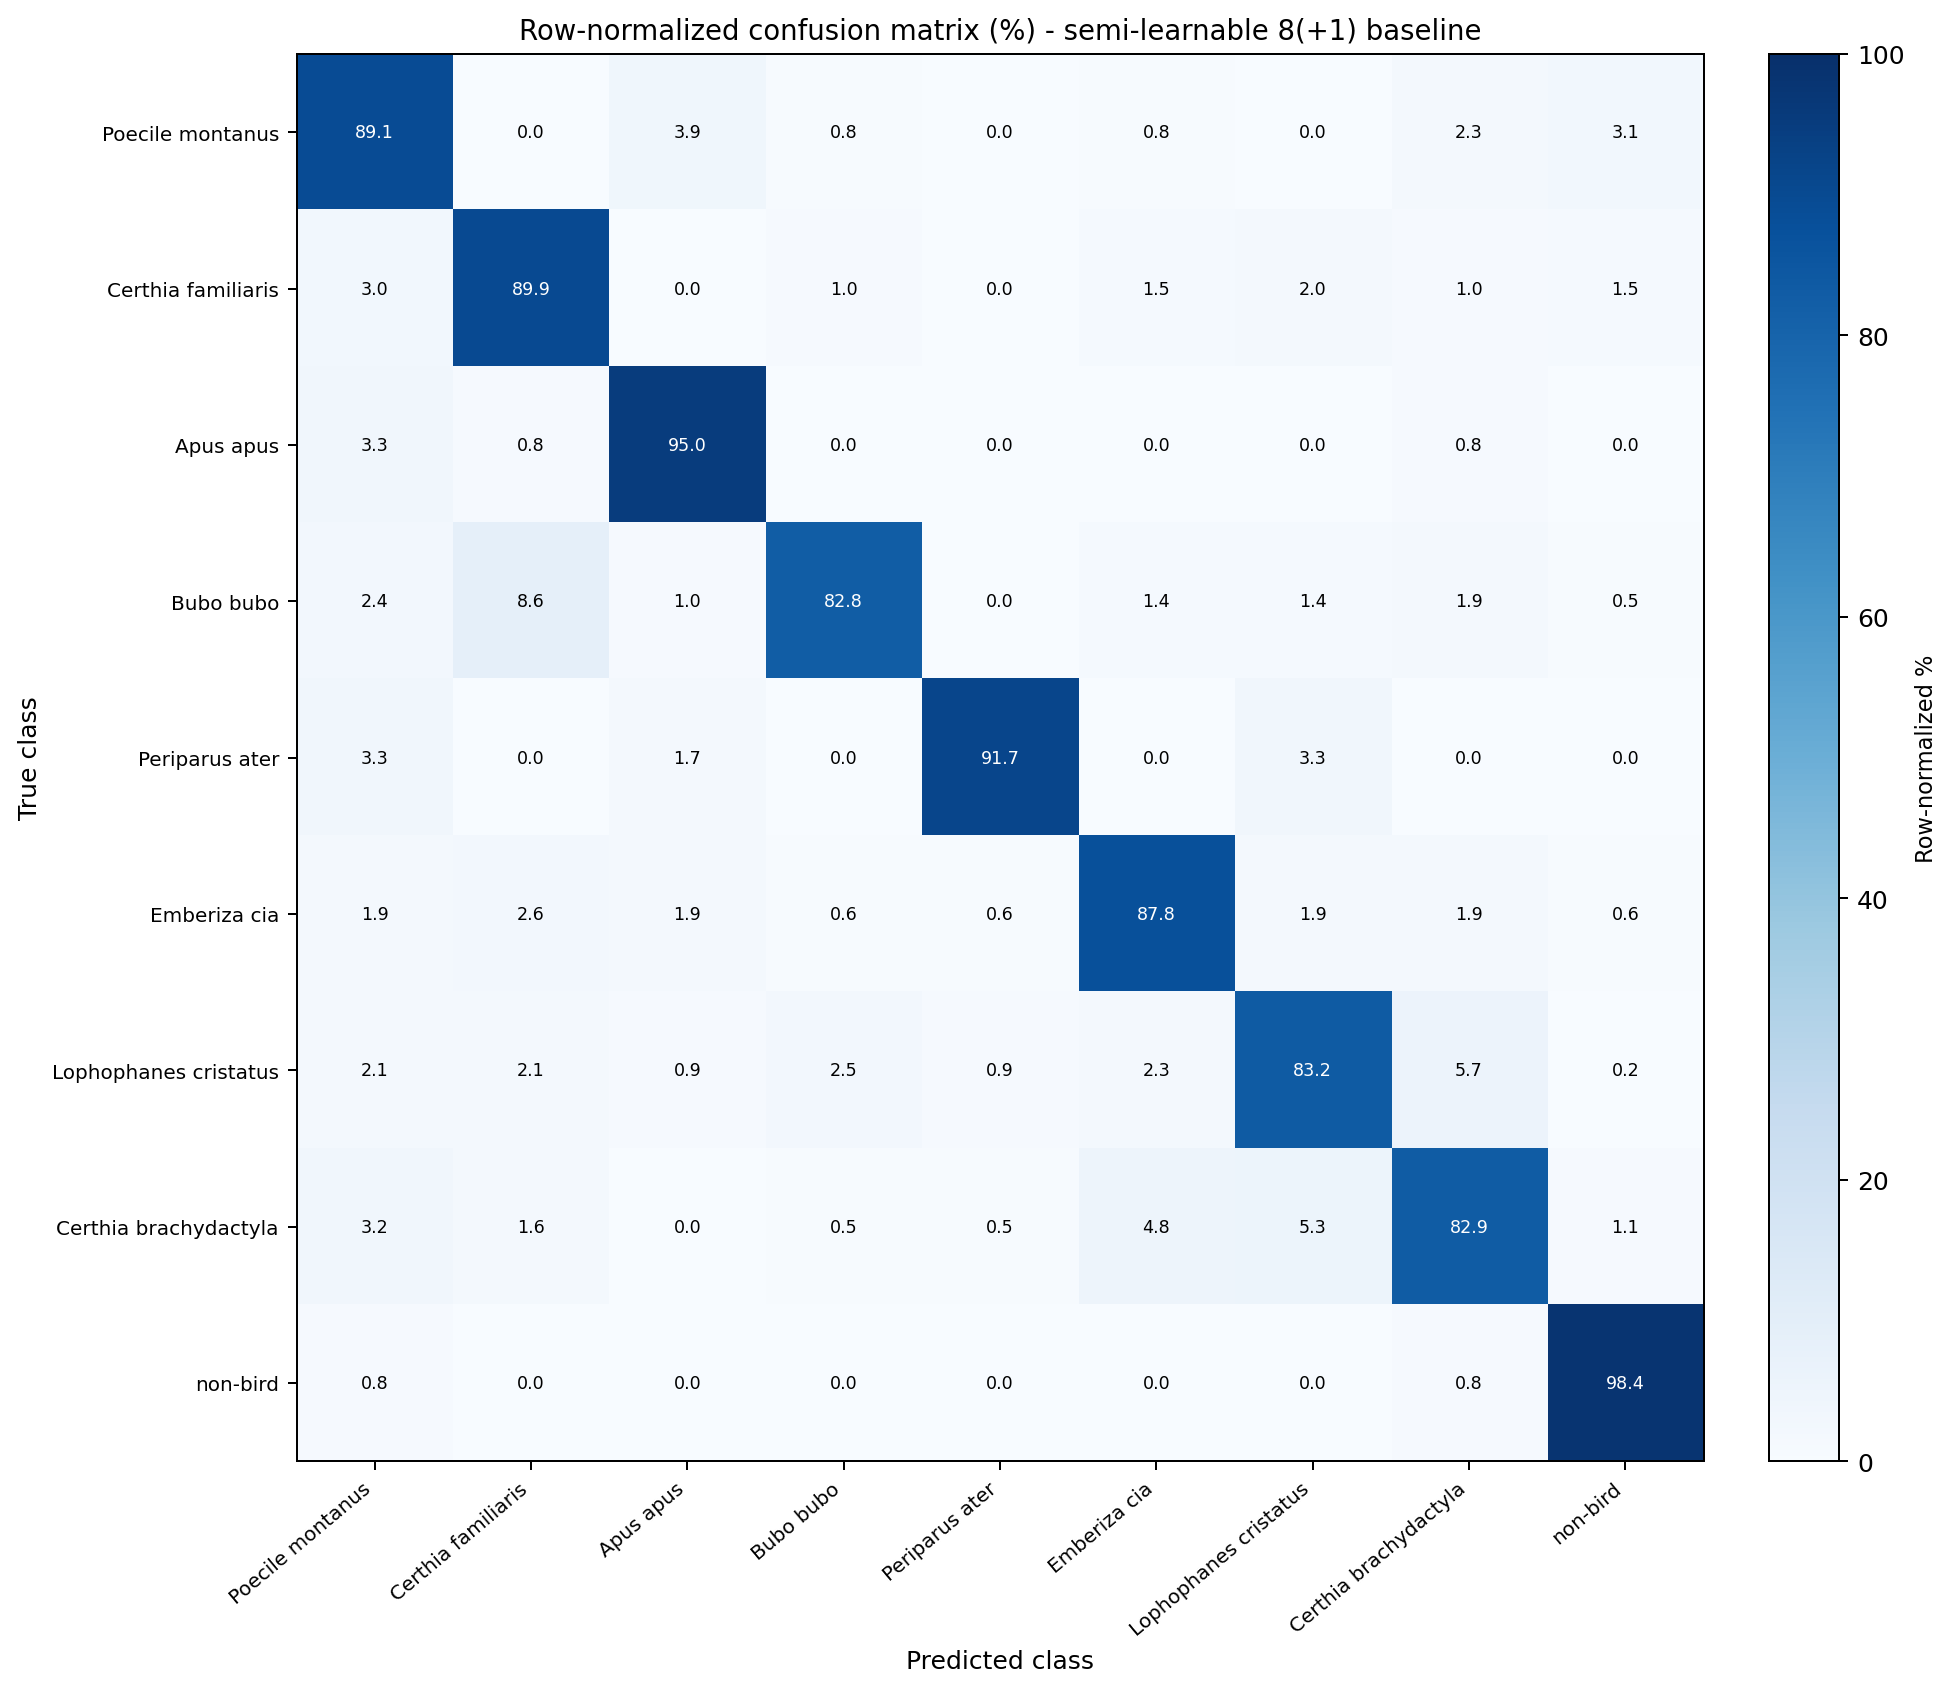
\includegraphics[width=0.70\textwidth]{images/confmat_8plus1_semi_rownorm.png}
			\caption[Confusion matrix for the controlled \(8(+1)\) semi-learnable baseline.]{Row-normalized confusion matrix (\%) for the controlled \(8(+1)\) semi-learnable baseline configuration.}
			\label{fig:confmat_8plus1_semi}
		\end{figure}

		\begin{figure}[H]
			\centering
			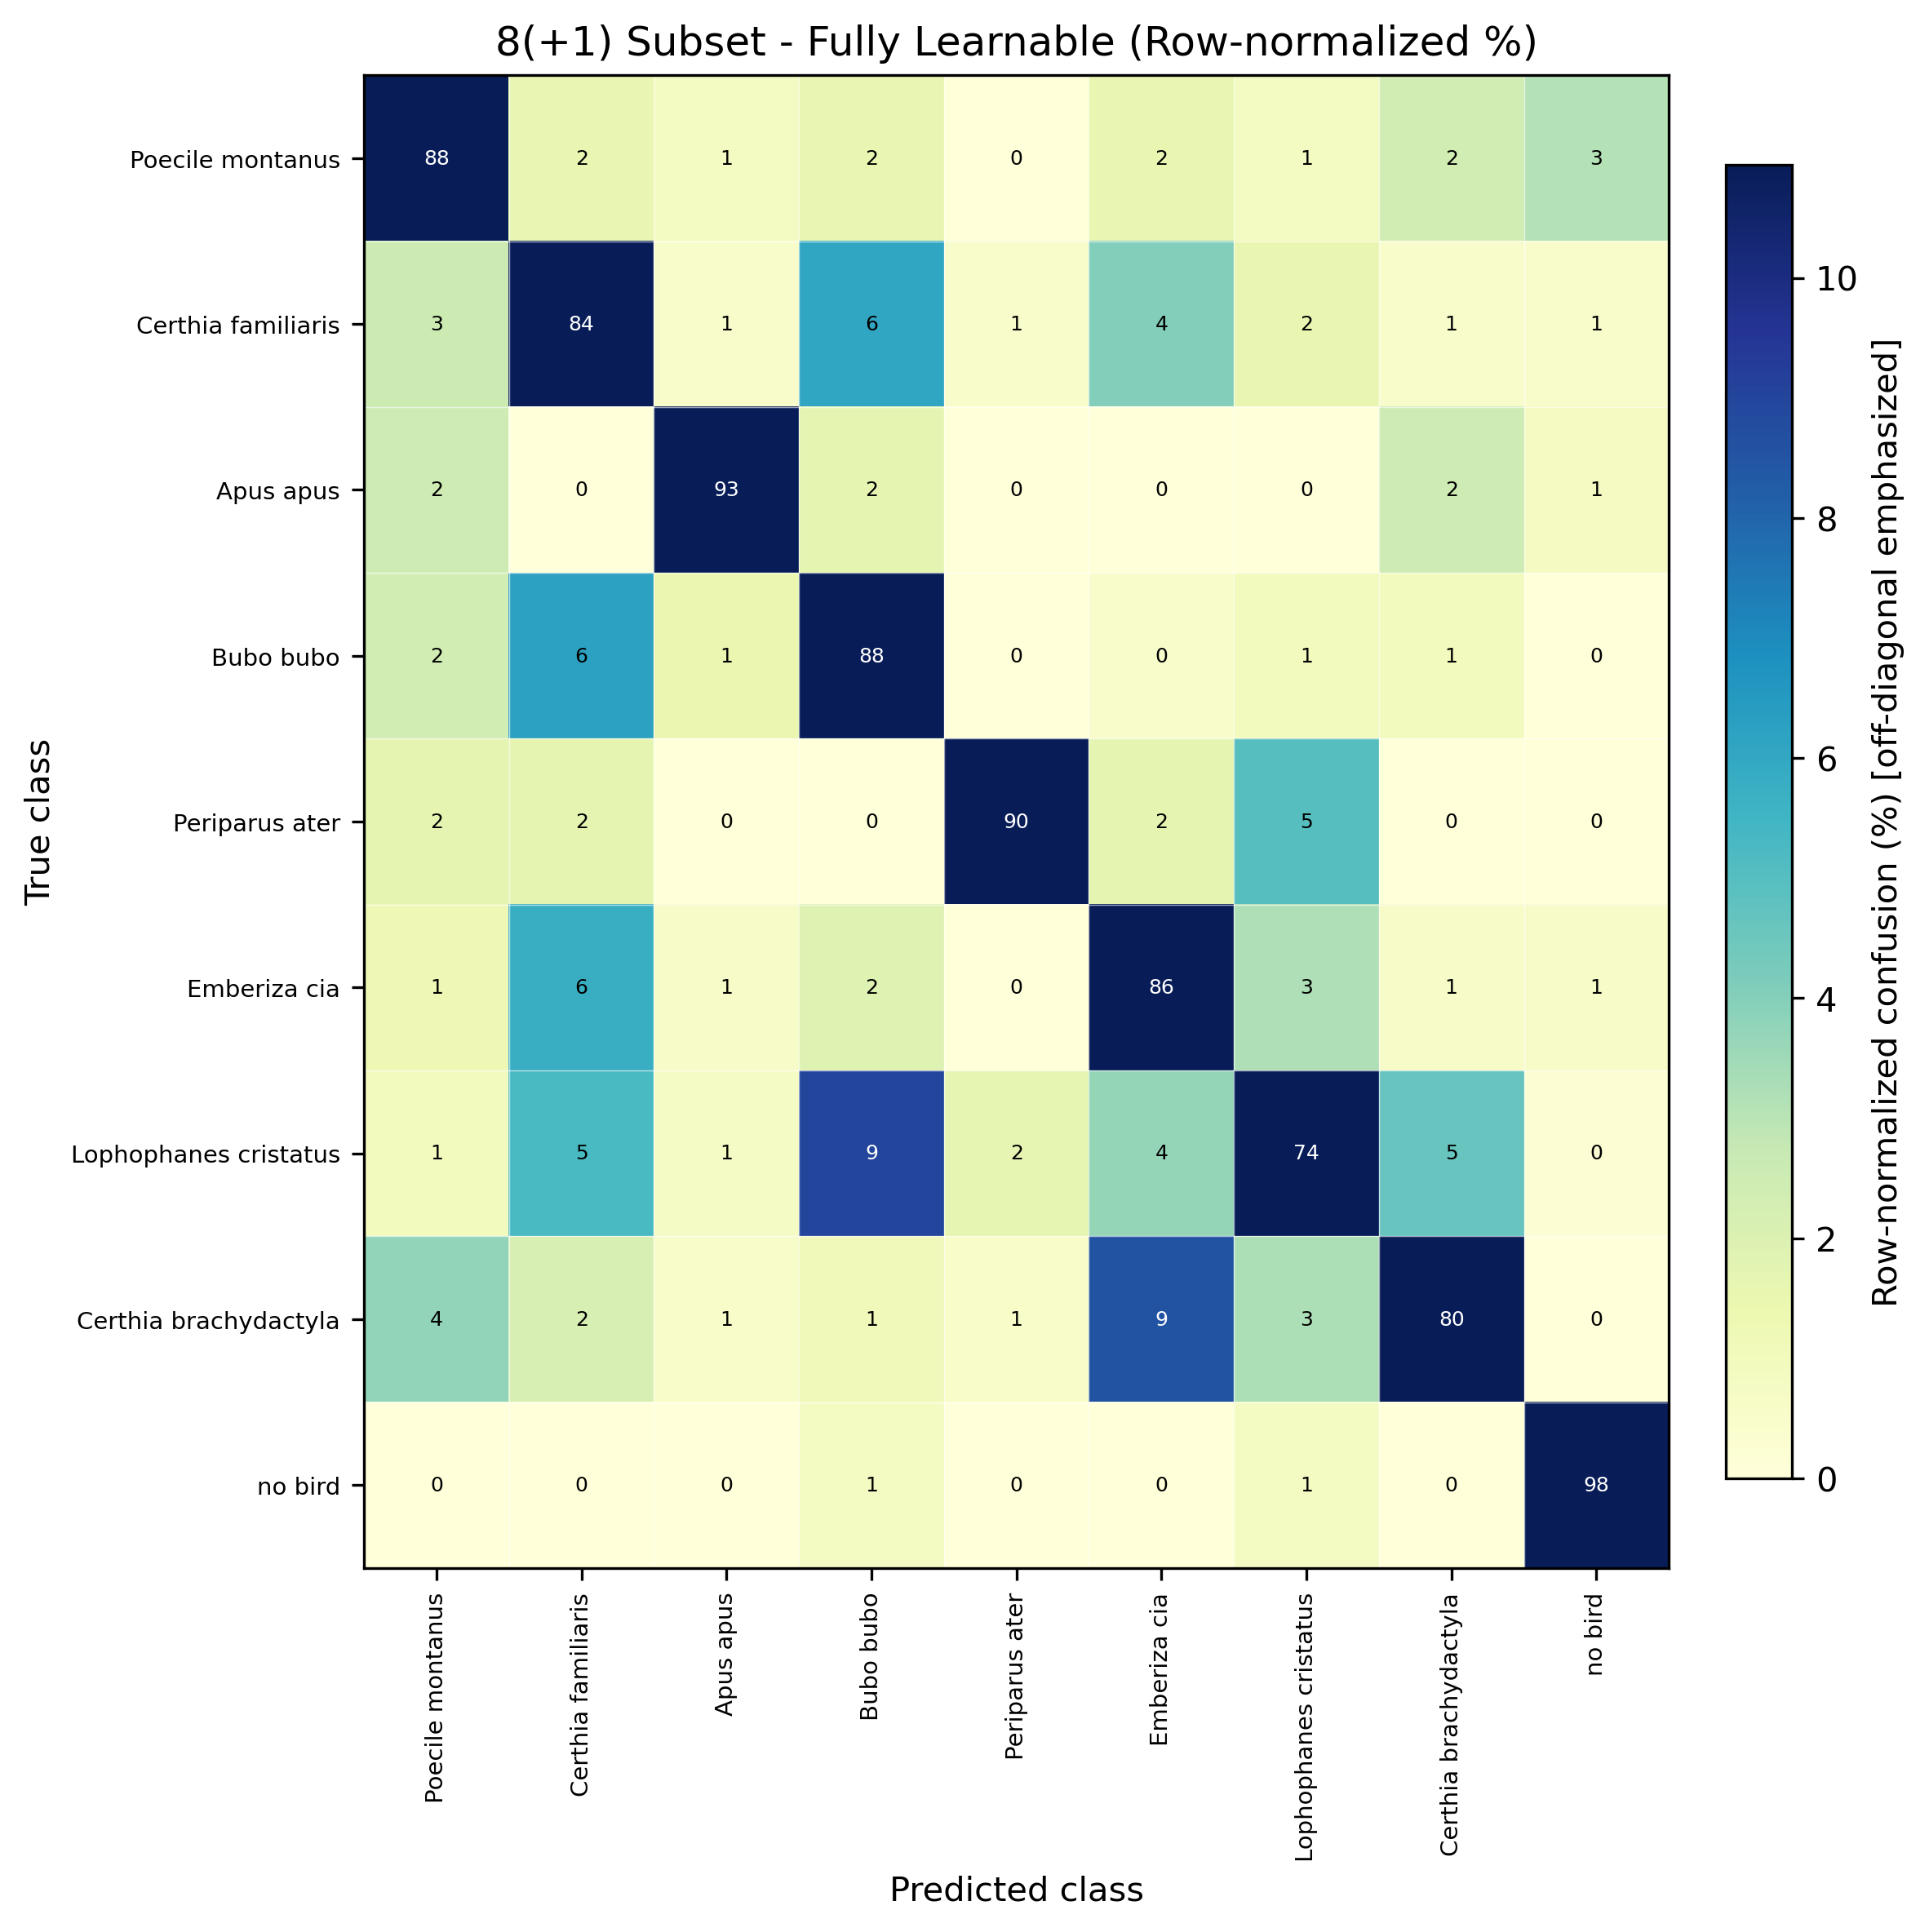
\includegraphics[width=0.70\textwidth]{images/confmat_8plus1_fully_rownorm.png}
			\caption[Confusion matrix for the controlled \(8(+1)\) fully learnable setup.]{Row-normalized confusion matrix (\%) for the controlled \(8(+1)\) fully learnable configuration.}
			\label{fig:confmat_8plus1_fully}
		\end{figure}
		\end{samepage}

		\begin{samepage}
		\begin{figure}[H]
			\centering
			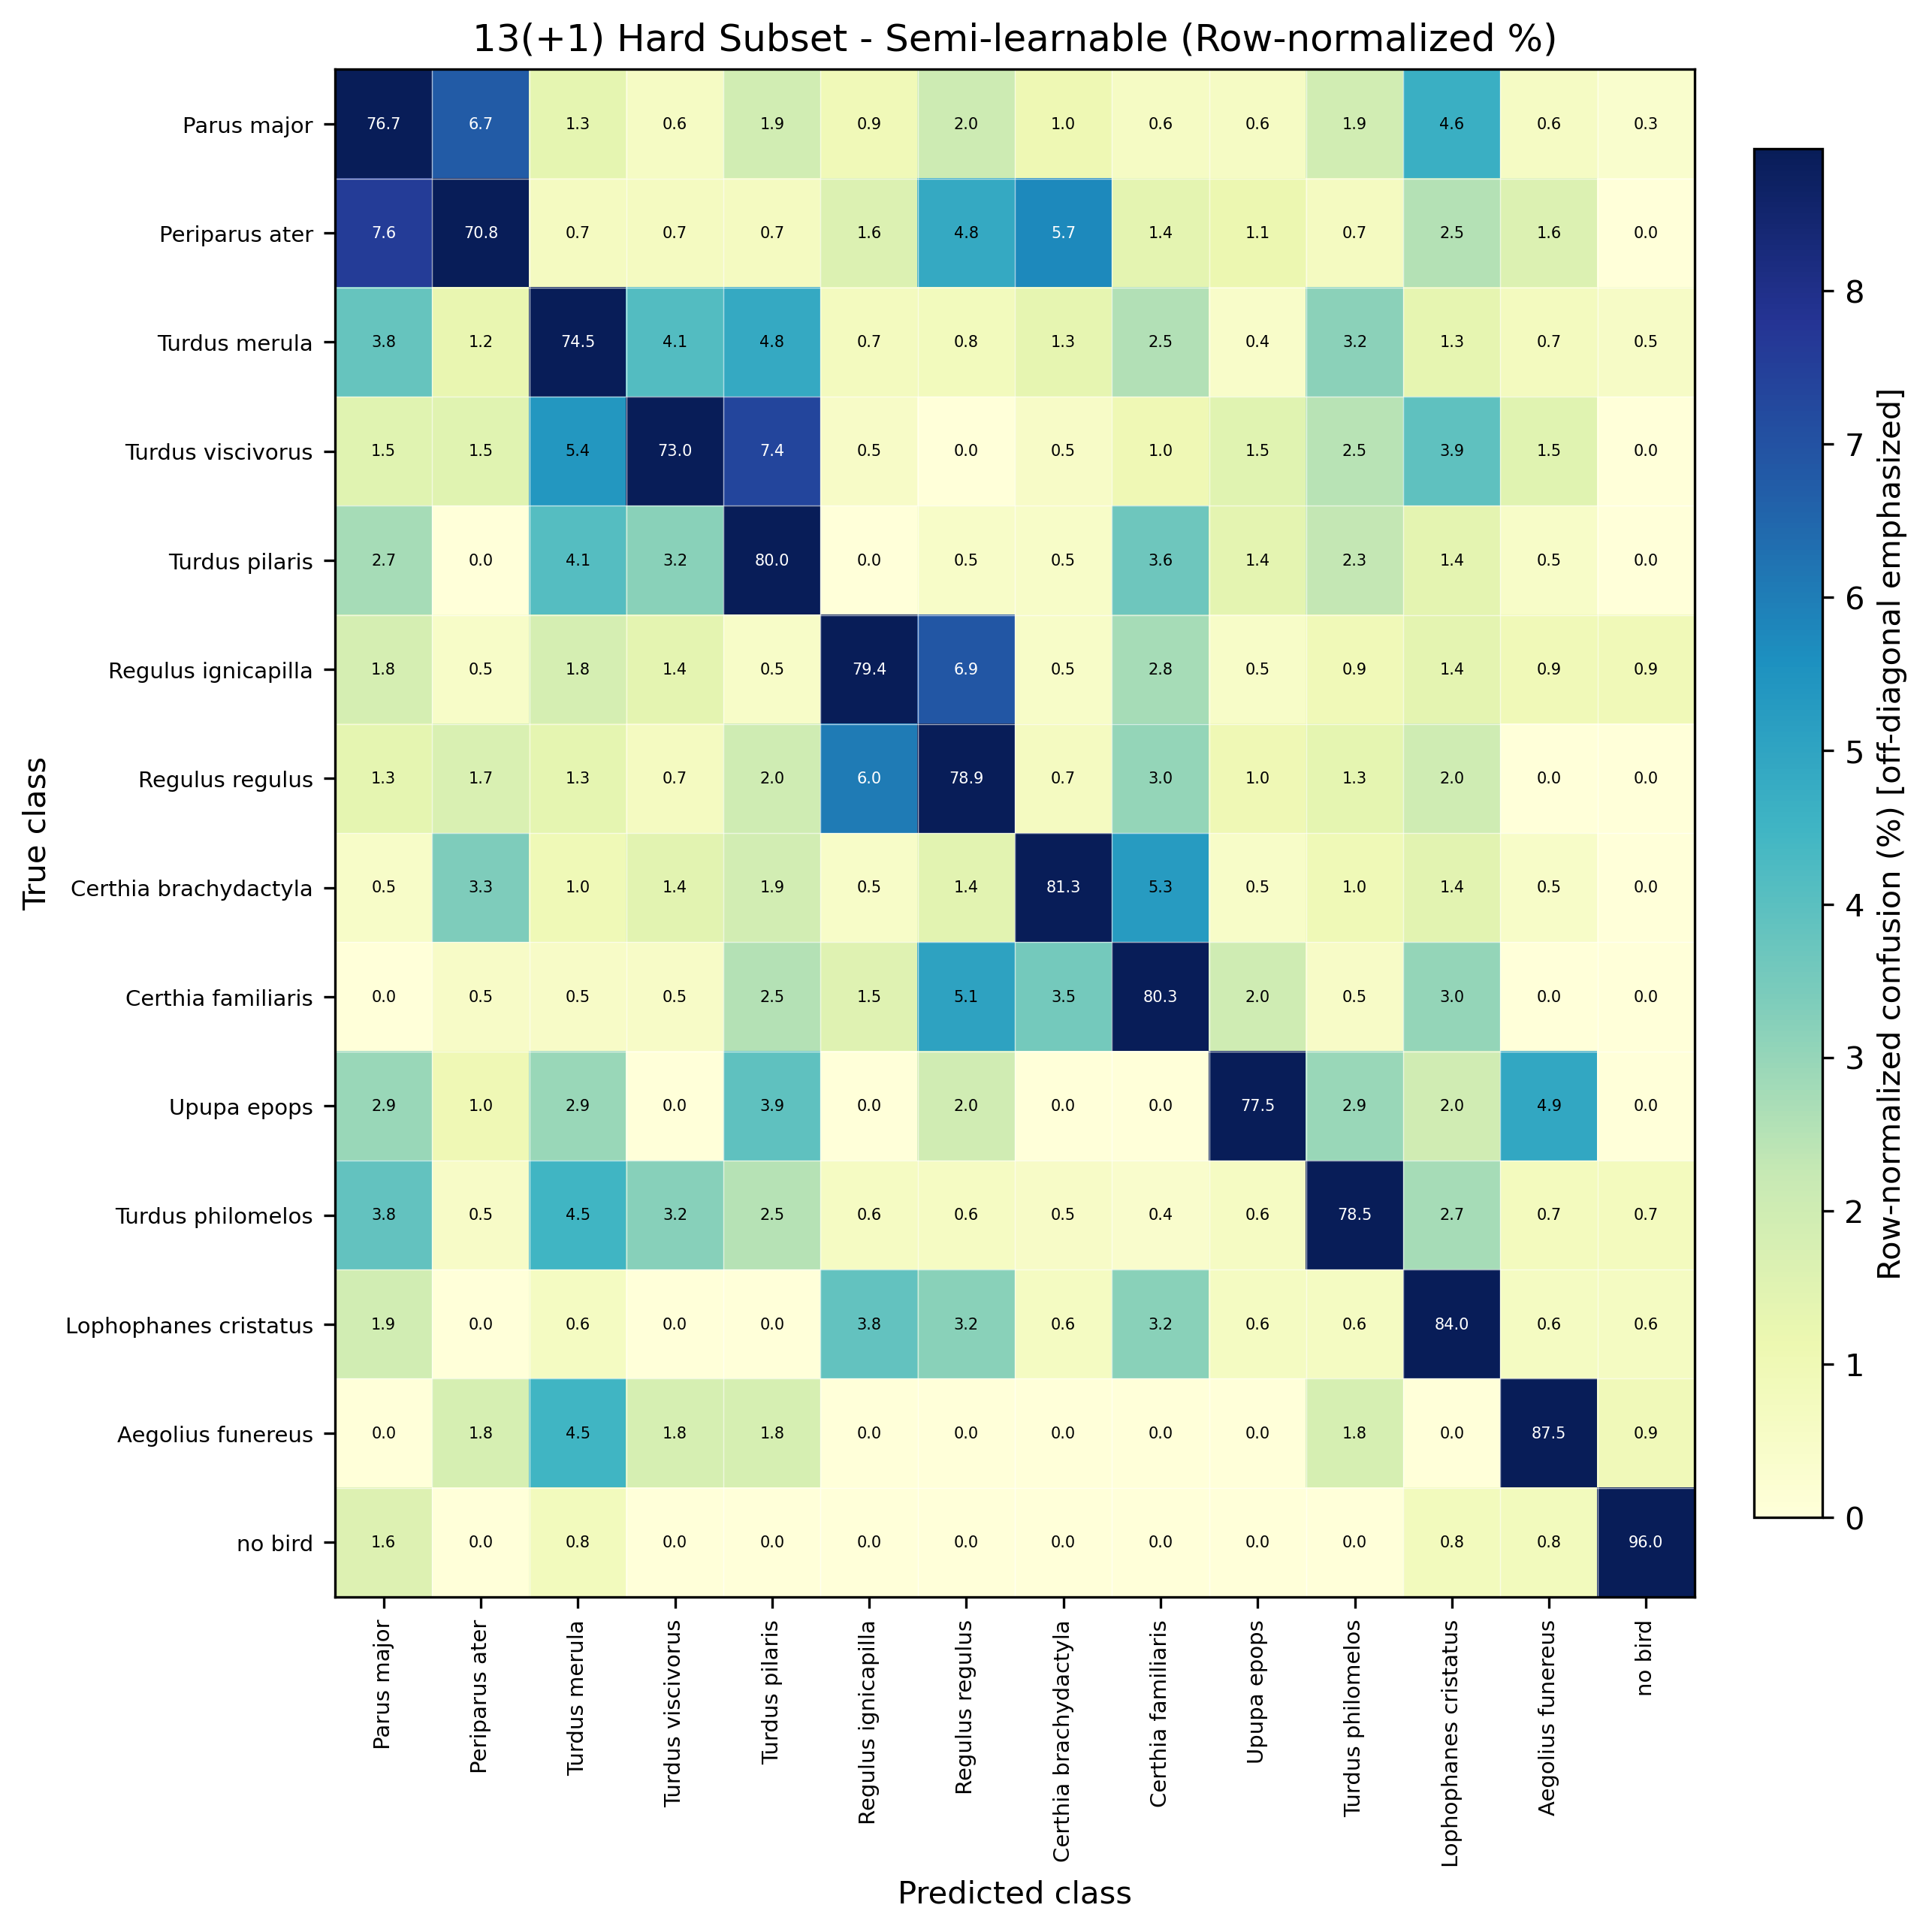
\includegraphics[width=0.64\textwidth]{images/confmat_13plus1_hard_rownorm.png}
			\caption[Confusion matrix for the \(13(+1)\) hard-species subset.]{Row-normalized confusion matrix (\%) for the \(13(+1)\) hard-species subset.}
			\label{fig:confmat_13plus1_hard}
		\end{figure}

		\vspace{-0.6em}
		\begin{figure}[H]
			\centering
			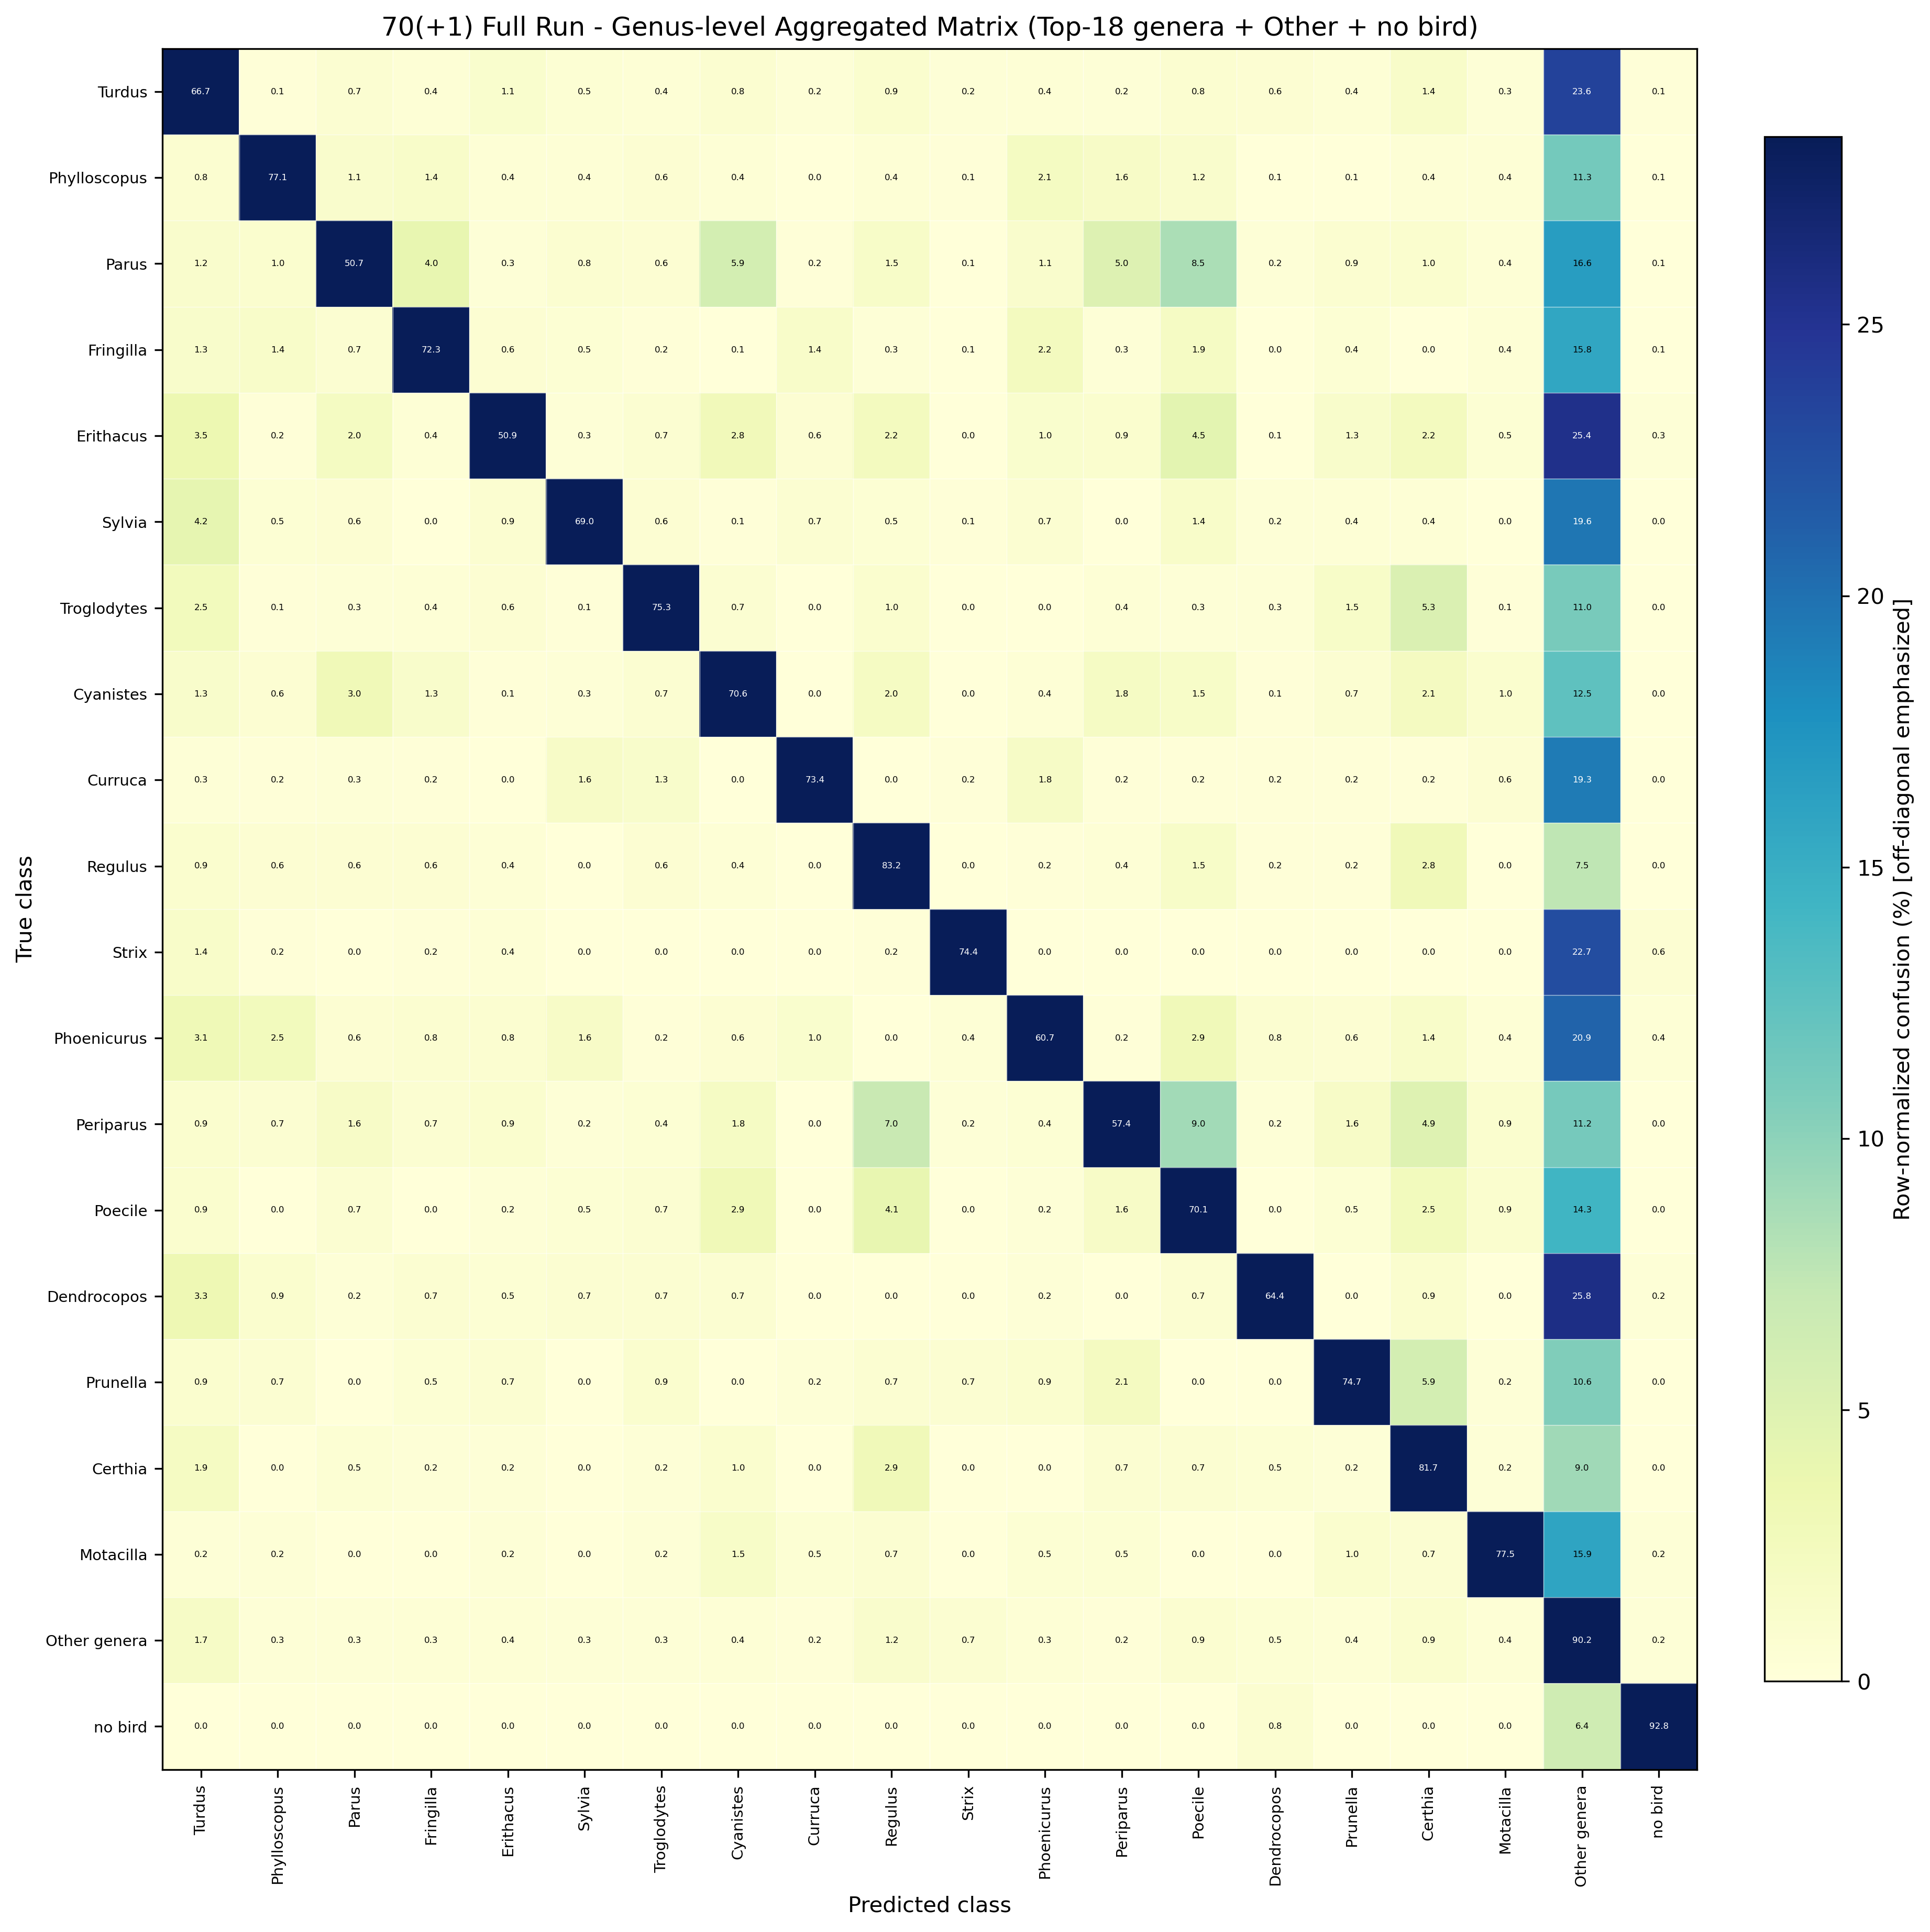
\includegraphics[width=0.64\textwidth]{images/confmat_70plus1_genus_aggregated_rownorm.png}
			\caption[Genus-level aggregated confusion matrix for the full dataset.]{Genus-level aggregated row-normalized confusion matrix (\%) for the \(70(+1)\) full-dataset setting (top-18 genera by support, plus ``Other genera'' and ``no bird'').}
			\label{fig:confmat_70plus1_genus}
		\end{figure}
		\end{samepage}

	The controlled \(8(+1)\) semi-learnable and fully learnable matrices confirm that errors are not uniformly distributed: the strongest directional confusion is \emph{Lophophanes cristatus} \(\rightarrow\) \emph{Bubo bubo} (about \(9\%\) of \emph{Lophophanes} samples), followed by \emph{Certhia brachydactyla} \(\rightarrow\) \emph{Emberiza cia} (about \(8.6\%\)). In the \(13(+1)\) hard subset, the dominant errors concentrate on expected difficult pairs, especially \emph{Parus major} \(\leftrightarrow\) \emph{Periparus ater} and \emph{Regulus ignicapilla} \(\leftrightarrow\) \emph{Regulus regulus}, with reciprocal confusion around \(6\%\) to \(8\%\).

	At full scale, genus aggregation makes long-tail behavior interpretable: part of the error mass is absorbed by the ``Other genera'' bucket, while within the top genera the most recurrent cross-genus spillovers involve \emph{Periparus} \(\rightarrow\) \emph{Poecile}, \emph{Parus} \(\rightarrow\) \emph{Poecile}, and \emph{Parus} \(\rightarrow\) \emph{Cyanistes}.

	The filterbank comparison clarifies why the combined log--linear solution is preferred to a fully learnable front-end. Across both the standard comparison and the controlled front-end study (Tables~\ref{tab:filterbank_comparison}, \ref{tab:semi_vs_fully_complexity}, and \ref{tab:semi_vs_fully_metrics}), the semi-learnable version remains consistently stronger while preserving a more compact and structured parameterization. Fully learnable filters expose a larger unconstrained search space and require substantially higher optimization effort for front-end coefficients, increasing computational cost and overfitting risk without clear gains in the present setup. The combined log--linear formulation instead keeps strong spectral priors, learns only the most relevant global adaptations, and therefore delivers a better accuracy/complexity trade-off.

	Beyond aggregate tables, detailed subset analysis reinforces the same conclusion. In monoclass settings, the model reaches \(92.37\%\) on \emph{Corvus corax} and \(94.71\%\) on \emph{Upupa epops}, with markedly different learned breakpoints (\(\sim 1955\)~Hz and \(\sim 5269\)~Hz), indicating species-dependent spectral allocation. On the hard two-species \emph{Regulus} pair, performance remains \(85.64\%\), showing that the architecture can preserve discriminative power even for acoustically similar classes when supervision is focused.

	Frequency-focused subsets show a consistent pattern. The high-frequency subset reaches \(91.49\%\) with learned breakpoint around \(164\)~Hz, while the low-frequency subset reaches \(91.63\%\) with breakpoint around \(237\)~Hz. In both cases, the mapping approaches near-linear behavior over most of the operative band, which supports the interpretation that the front-end is adapting to the dominant spectral demands of the active class set, instead of just converging to one fixed prior.

	At full scale, the compact model reaches \(66.51\%\) with approximately \(57\)k parameters, while a larger \(136\)k-parameter variant reaches \(70.14\%\). The absolute gain is \(3.6\) percentage points, but with substantially higher model capacity. This confirms a central result: larger capacity improves full-task accuracy, yet compact semi-learnable designs still retain a favorable operating point when constrained deployment remains a primary objective.

	At full scale, the compact model remains competitive while preserving deployment constraints, whereas the larger model recovers additional accuracy at significantly higher complexity. This confirms the expected trade-off: as class count and inter-class overlap grow, absolute performance improves with capacity, but deployment cost becomes harder to sustain on low-power devices.
	\subsubsection{Error Analysis}
	Error patterns are not uniformly distributed across classes. The highest confusion appears in taxonomically or acoustically similar groups, especially in subsets explicitly designed as difficult. This is coherent with the front-end and architecture analysis: the model learns useful discriminative structure, but near-overlapping vocal signatures remain the hardest regime.

	\begin{table}[p]
\centering
\scriptsize
\caption{Top-10 symmetric confusion pairs on the controlled \(8(+1)\) subset: semi-learnable baseline versus fully learnable front-end. Percentages are pair confusion rates normalized by the two-class support of each pair.}
\label{tab:top10_confusion_pairs}
\begin{tabular}{|p{4.9cm}|r|r|r|r|r|}
\hline
Species pair & Semi cnt & Semi \% & Fully cnt & Fully \% & \(\Delta\) Fully-Semi \\
\hline
Lophophanes cristatus \(\leftrightarrow\) Certhia brachydactyla & 35 & 5.63 & 26 & 4.18 & -9 (-1.45 pp) \\
\hline
Bubo bubo \(\leftrightarrow\) Lophophanes cristatus & 14 & 2.17 & 41 & 6.37 & +27 (+4.19 pp) \\
\hline
Certhia familiaris \(\leftrightarrow\) Bubo bubo & 20 & 4.91 & 25 & 6.14 & +5 (+1.23 pp) \\
\hline
Certhia familiaris \(\leftrightarrow\) Lophophanes cristatus & 13 & 2.05 & 26 & 4.11 & +13 (+2.05 pp) \\
\hline
Emberiza cia \(\leftrightarrow\) Lophophanes cristatus & 13 & 2.20 & 21 & 3.55 & +8 (+1.35 pp) \\
\hline
Emberiza cia \(\leftrightarrow\) Certhia brachydactyla & 12 & 3.50 & 17 & 4.96 & +5 (+1.46 pp) \\
\hline
Certhia familiaris \(\leftrightarrow\) Emberiza cia & 7 & 1.98 & 17 & 4.80 & +10 (+2.82 pp) \\
\hline
Poecile montanus \(\leftrightarrow\) Certhia brachydactyla & 9 & 2.85 & 10 & 3.16 & +1 (+0.32 pp) \\
\hline
Periparus ater \(\leftrightarrow\) Lophophanes cristatus & 6 & 1.21 & 10 & 2.02 & +4 (+0.81 pp) \\
\hline
Poecile montanus \(\leftrightarrow\) Lophophanes cristatus & 9 & 1.60 & 5 & 0.89 & -4 (-0.71 pp) \\
\hline
\end{tabular}
\end{table}

	In Table~\ref{tab:top10_confusion_pairs}, \(N\) indicates the number of symmetric pair-confusion events, \(R\) indicates the corresponding normalized confusion rate, and the \(\Delta\) columns report the change from fully learnable minus semi-learnable. Positive deltas mean higher confusion in the fully learnable variant, while negative deltas indicate an improvement. The table quantifies how pair-specific confusion changes on the controlled \(8(+1)\) subset: some pairs improve (for example \emph{Lophophanes cristatus} \(\leftrightarrow\) \emph{Certhia brachydactyla}), while others become substantially worse (for example \emph{Bubo bubo} \(\leftrightarrow\) \emph{Lophophanes cristatus}).

	\begin{table}[H]
		\centering
		\scriptsize
		\renewcommand{\arraystretch}{1.15}
		\setlength{\tabcolsep}{6pt}
		\caption{Analysis of difficult species pairs and genus-level confusion patterns.}
		\label{tab:difficult_species_pairs}
		\resizebox{\textwidth}{!}{%
		\begin{tabular}{|p{3.3cm}|c|p{2.9cm}|p{6.2cm}|}
			\hline
			Pair or Species & Recall (\%) & Pair Verdict & Details on Confusion \\
			\hline
			\emph{Parus} / \emph{Periparus} & -- & Both Very Difficult & Strong mutual confusion and spillover confusion with multiple additional species. \\
			\hline
			\emph{Parus major} (Great Tit) & 62.6 & -- & Mistaken for \emph{Periparus ater} (46 times) and \emph{Fringilla coelebs} (49 times). \\
			\hline
			\emph{Periparus ater} (Coal Tit) & 66.3 & -- & Mistaken for \emph{Parus major} (18 times). \\
			\hline
			\emph{Turdus} genus & -- & Genus Problem & Strong cross-confusion among thrush species. \\
			\hline
			\emph{Turdus merula} (Blackbird) & 68.8 & -- & Confused with \emph{Turdus philomelos} (21 times) and \emph{Turdus pilaris} (37 times). \\
			\hline
			\emph{Turdus viscivorus} (Mistle Thrush) & 72.4 & -- & Similar intra-genus confusion pattern. \\
			\hline
			\emph{Regulus} genus & -- & Mutual Confusion & Main source of error is reciprocal confusion between the two \emph{Regulus} species. \\
			\hline
			\emph{Regulus ignicapilla} (Firecrest) & 72.5 & -- & Mistaken for \emph{Regulus regulus} in approximately 13\% of cases. \\
			\hline
			\emph{Regulus regulus} (Goldcrest) & 74.0 & -- & Mistaken for \emph{Regulus ignicapilla} in approximately 6.7\% of cases. \\
			\hline
			\emph{Certhia} genus & -- & \emph{C. familiaris} Hardest & Asymmetric confusion between the two treecreeper species. \\
			\hline
			\emph{Certhia brachydactyla} (Short-toed Treecreeper) & 79.0 & -- & Mostly confused with \emph{Certhia familiaris}. \\
			\hline
			\emph{Certhia familiaris} (Eurasian Treecreeper) & 71.7 & -- & Lower recall and confusion with a wider set of species. \\
			\hline
		\end{tabular}
		}
	\end{table}

	\begin{table}[H]
		\centering
		\scriptsize
		\renewcommand{\arraystretch}{1.15}
		\setlength{\tabcolsep}{6pt}
		\caption{Analysis of species in the easy subset.}
		\label{tab:easy_species_analysis}
		\resizebox{\textwidth}{!}{%
		\begin{tabular}{|p{3.3cm}|c|p{2.9cm}|p{6.2cm}|}
			\hline
			Species & Recall (\%) & Verdict & Why It Is Easy \\
			\hline
			non-bird & 91.9 & Very Easy & Easy to detect the absence of bird vocalizations. \\
			\hline
			\emph{Corvus corax} (Common Raven) & 88.5 & Very Easy & Distinct low-frequency vocal profile. \\
			\hline
			\emph{Falco tinnunculus} (Kestrel) & 86.5 & Very Easy & Sharp repetitive call pattern. \\
			\hline
			\emph{Otus scops} (Scops Owl) & 86.4 & Very Easy & Simple rhythmic whistle with high regularity. \\
			\hline
			\emph{Hirundo rustica} (Barn Swallow) & 86.1 & Easy & Fast chirping pattern with recognizable temporal structure. \\
			\hline
			\emph{Phylloscopus collybita} (Chiffchaff) & 85.1 & Easy & Characteristic repetitive ``chip-chop'' motif. \\
			\hline
			\emph{Ardea cinerea} (Grey Heron) & 84.0 & Easy & Harsh croaking call with clear spectral profile. \\
			\hline
			\emph{Picus canus} (Grey-headed Woodpecker) & 84.0 & Easy & Loud structured calls with stable acoustic signature. \\
			\hline
			\emph{Strix aluco} (Tawny Owl) & 82.7 & Easy & Iconic hoot pattern, acoustically distinct. \\
			\hline
		\end{tabular}
		}
	\end{table}

	The ``no bird'' class plays a central role in practical operation. False positives in this class directly affect field usability by increasing unnecessary storage and manual review. The negative-class construction strategy described earlier reduces this risk by combining environmental negatives and in-domain empty segments, but residual errors remain expected under very low-SNR or strongly overlapping soundscapes.
	\subsubsection{Accuracy-Efficiency Trade-Offs}
		\begin{sloppypar}
		Deployment-level comparison confirms that efficiency must be evaluated jointly with recognition metrics. The compact student configuration yields a much stronger practical profile than heavy baselines when measured on edge-relevant hardware and fixed 3-second inference windows. In this setting, the key quantity is not only absolute classification quality, but the energy required to obtain each prediction.
		\end{sloppypar}

	The detailed benchmarking protocol, raw electrical measurements, and instrumentation figures are reported in Section~\ref{sec:device_benchmarks}. In summary, relative to Raspberry Pi 3B+ student TFLite inference (\(0.1720\)~J per window), the AudioMoth deployment (\(0.0771\)~J) reduces energy per inference by about \(55\%\). Relative to the Raspberry Pi student STFT baseline (\(1.6500\)~J) and the BirdNET baseline (\(2.7900\)~J), the reductions are about \(95.3\%\) and \(97.2\%\), respectively. The BirdNET gap corresponds to a \(36.2\times\) lower energy cost in this setup.

\subsection{AudioMoth Deployment}
\subsubsection{AudioMoth Platform Characteristics}
		\begin{sloppypar}
		The deployment target is AudioMoth Dev, chosen for long-duration field recording and low-power embedded operation. In this project, it is used as a microcontroller-class platform for on-device inference under strict memory and power constraints. The key hardware characteristics reported below are taken from the official AudioMoth Dev 1.0.1 datasheet \cite{audiomothdev2023}, while the broader device context for biodiversity monitoring is discussed in prior AudioMoth work \cite{audiomoth2019}.
		\end{sloppypar}

		AudioMoth is part of an open-source project developed to make large-scale acoustic monitoring more accessible in ecology and conservation. Its adoption in the field has been driven by a combination of low cost, battery-powered operation, simple deployment logistics, and broad reuse across biodiversity studies \cite{audiomoth2019}. These characteristics are directly relevant to the present thesis. They align with the practical goal of running useful acoustic intelligence on small devices that can be deployed in high numbers, repurposed across campaigns, and maintained with lower overall infrastructure cost than more compute-heavy platforms.

	\begin{figure}[H]
		\centering
		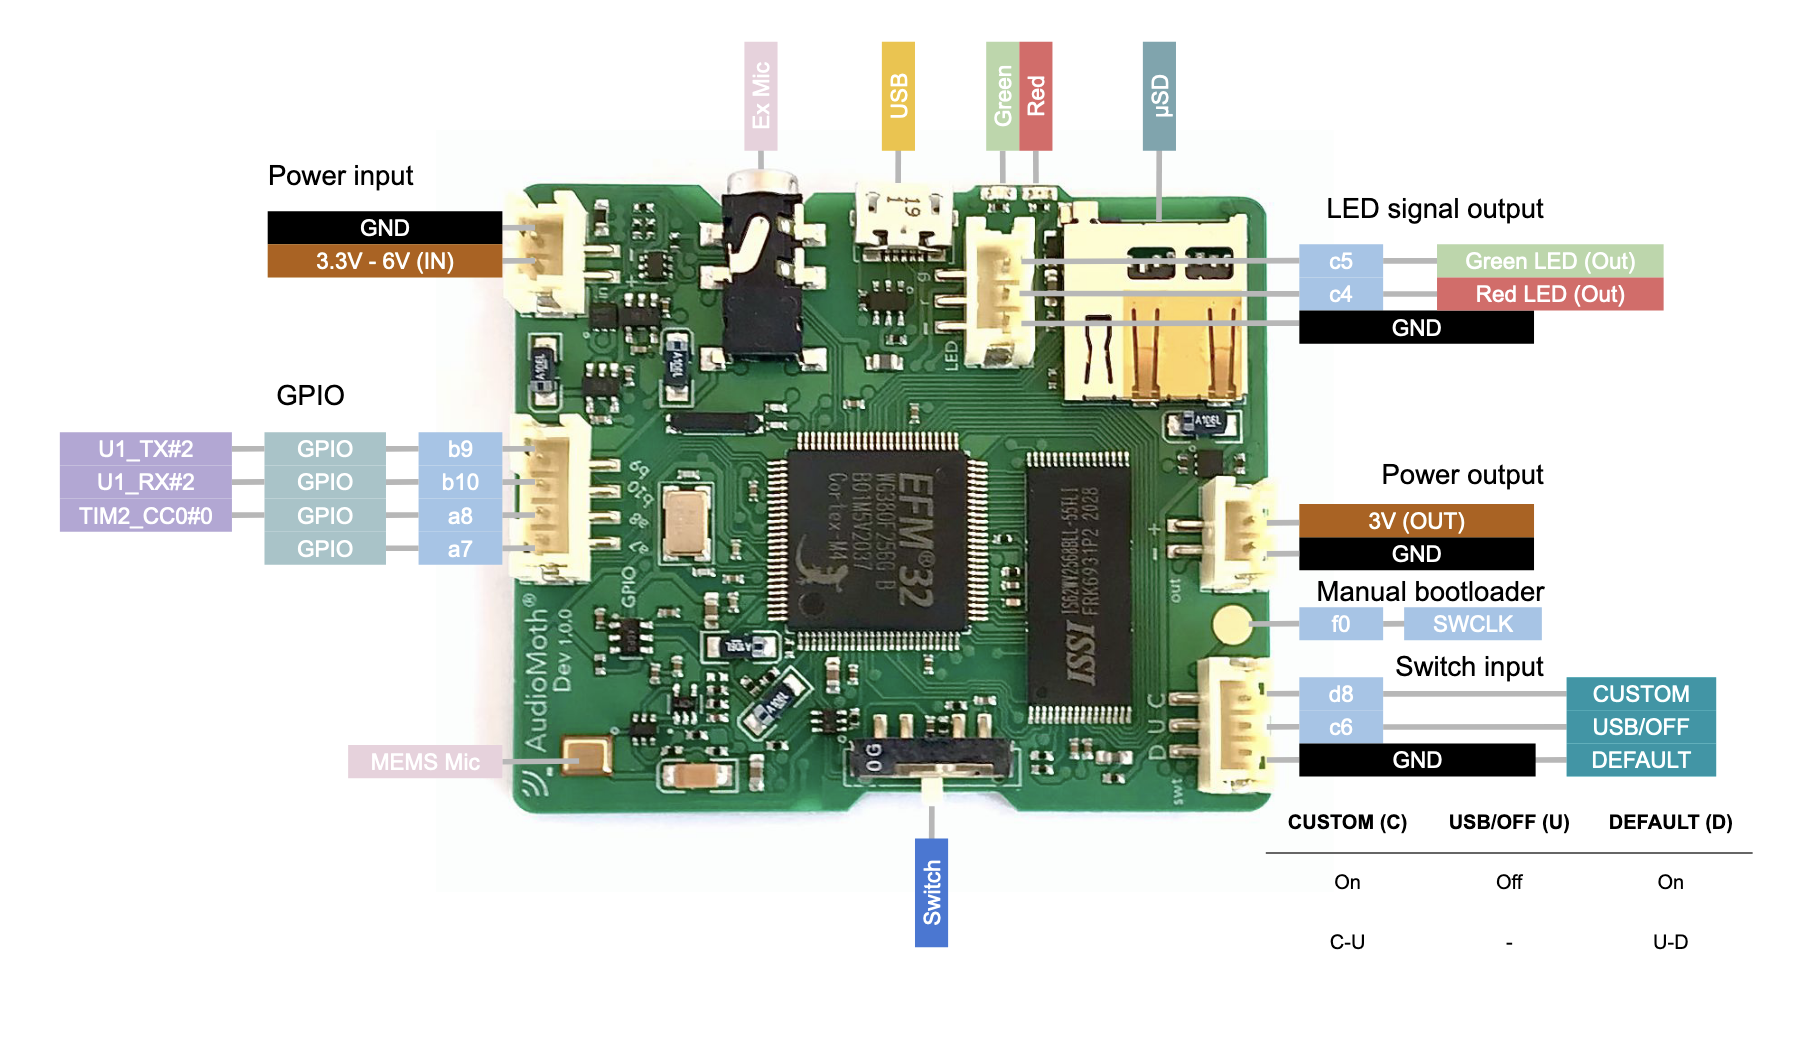
\includegraphics[width=0.78\textwidth]{images/audiomoth_top.png}
		\vspace{0.6em}
		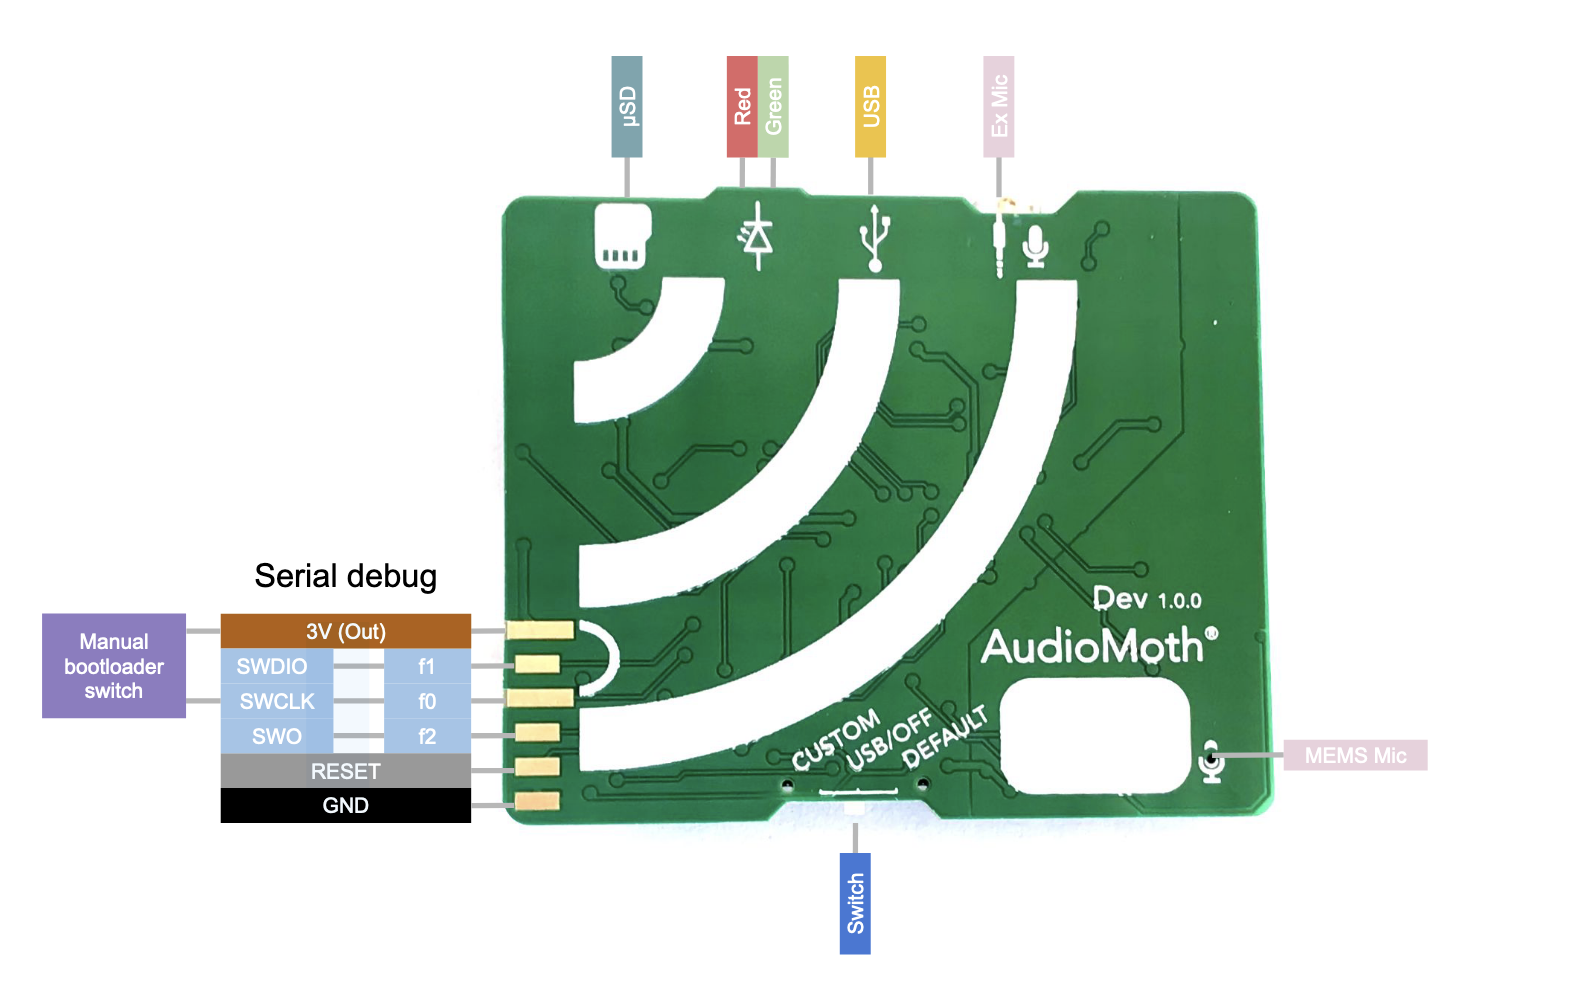
\includegraphics[width=0.78\textwidth]{images/audiomoth_down.png}
		\caption[AudioMoth hardware used for deployment tests.]{AudioMoth hardware used for on-device deployment tests. Top image: top view. Bottom image: bottom view.}
		\label{fig:audiomoth_hardware_views}
	\end{figure}

	The two views in Figure~\ref{fig:audiomoth_hardware_views} show the physical layout of the board used in this thesis. These constraints directly affect firmware design, memory partitioning, and feasible inference scheduling.

	\begin{table}[H]
		\centering
		\scriptsize
		\renewcommand{\arraystretch}{1.15}
		\setlength{\tabcolsep}{6pt}
		\caption[Main technical characteristics of the AudioMoth Dev platform.]{Main technical characteristics of the AudioMoth Dev platform used in this work \cite{audiomothdev2023}.}
		\label{tab:audiomoth_specs}
		\begin{tabular}{|l|p{9.0cm}|}
			\hline
			Processing core & Silicon Labs EFM32WG380F256 (ARM Cortex-M4F), up to 48~MHz, DSP instruction support, floating-point unit \\
			\hline
			On-chip memory & 256~kB Flash and 32~kB RAM \\
			\hline
			External memory & 256~kB external SRAM (used for buffering and tensor arena allocation) \\
			\hline
			On-board microphone & Analog MEMS SPU0410LR5H-QB, sensitivity around \(-38\)~dBV/Pa, SNR \(63\)~dB(A), nominal band 10~Hz--192~kHz \\
			\hline
			Sampling capability & Configurable sample rates up to 384~kHz \\
			\hline
			Storage & microSD support up to 1~TB (exFAT) \\
			\hline
			Power input & 3.3~V to 6~V input range \\
			\hline
			Mechanical size & Approximately \(58 \times 48 \times 8\)~mm \\
			\hline
		\end{tabular}
	\end{table}

\subsubsection{Firmware and Library Integration}
	The deployment stack is integrated as an extension of the standard AudioMoth firmware, keeping the original device services (boot flow, timing, watchdog, DMA-based audio buffering, storage support) and adding a dedicated neural subsystem for embedded inference. This separation keeps low-level device control stable while allowing model-level updates without redesigning the full firmware architecture.

	The software toolchain is based on GNU Arm Embedded compilation for Cortex-M4, with size-oriented optimization and microcontroller-oriented TensorFlow Lite configuration flags. In practice, the firmware is linked with a constrained runtime profile where static allocation is preferred for predictable behavior, and where inference code is compiled together with the rest of the embedded application instead of being loaded dynamically.

		\begin{sloppypar}
		Library integration follows a layered design. At the base, the platform firmware and CMSIS components provide hardware abstraction and optimized integer kernels \cite{cmsisnn2018}. Above this layer, a lightweight model parser and bridge logic expose model metadata, tensor interfaces, quantization parameters, and operator dispatch to the application. The inference path uses two embedded model binaries, backbone and streaming, both exported as C arrays and initialized during firmware startup.
		\end{sloppypar}

	A key integration choice is explicit memory mapping through the linker. A dedicated tensor-arena section is reserved in external SRAM, and the neural subsystem partitions this region between backbone and streaming execution contexts. This avoids heap pressure in internal RAM and keeps runtime memory usage bounded. Initialization verifies arena availability and address validity before model activation, so memory faults are caught early.

	From an engineering perspective, robustness is handled jointly by initialization checks and runtime guards. Model-bridge construction is validated step by step, watchdog feeding is maintained during long operations, and fallback logic is present when a full bridge path cannot be initialized. The resulting firmware profile remains deterministic enough for repeated benchmarks and long-duration field sessions, while preserving the modularity needed for future model updates.

\subsubsection{On-Device Inference Pipeline}
	On AudioMoth, inference runs on fixed windows of 1024 samples. Each processing step starts with the backbone stage: the current int16 audio window is mapped to the backbone input tensor, the model is invoked, and a compact feature representation is produced for the temporal stage.

	The second stage runs the streaming model. It receives the current feature vector together with the recurrent hidden state carried from the previous window, then returns updated logits and the next hidden state. This state is preserved across consecutive windows and reset only during initialization or explicit reset paths. The effect is a temporally continuous decision process, which is important for bird vocalizations that are often identified by short sequences of motifs.

	Decision emission is handled in a dedicated post-processing step. Logits are stabilized and normalized with softmax, then filtered with the firmware confidence threshold (\texttt{0.7}) and with a hard cap on emitted detections per second (\texttt{2}). This gives deterministic runtime behavior and avoids bursty over-reporting.

	The firmware also enforces explicit state checks at every critical point of initialization and inference. Arena availability is validated before model startup, bridge/tensor pointers are verified before each invocation, and watchdog feeding is integrated in long-running loops. In case of failure, execution transitions to a controlled error state instead of continuing with undefined model outputs.

\subsubsection{INT8 Quantization for Deployment}
	Deployment uses two INT8 TensorFlow Lite models, one for backbone feature extraction and one for streaming classification. The quantized path is handled through the embedded bridge layer, which exposes tensor scale and zero-point metadata and keeps operator execution aligned with CMSIS-NN constraints.

	At runtime, conversions between int8 tensors and floating-point buffers are done only at well-defined interfaces. Backbone and streaming outputs are dequantized before softmax and decision logic, while model inputs remain in the integer pipeline expected by the interpreter. This keeps the deployed numerical flow consistent and traceable.

		\begin{sloppypar}
		Memory behavior is fully static. The external arena is reserved at firmware level, and the inference path uses fixed working partitions for the two stages, \(40\)~KiB for backbone and \(20\)~KiB for streaming, with preallocated bridge/tensor structures and no dynamic allocation during inference. This choice prevents heap fragmentation and keeps memory usage predictable across long monitoring runs.
		\end{sloppypar}

	The same INT8 configuration is used in repeated on-device benchmark loops, including stress runs with randomized input windows. This validates the quantized execution path under sustained conditions and confirms that the deployment stack is stable on the target hardware.

\subsection{Tests}
\subsubsection{Functional Tests on Device}
	Functional validation was performed as a hardware-in-the-loop protocol on the target microcontroller. The test sequence includes firmware flashing, controlled reset, breakpoint-assisted verification of initialization phases, and runtime checks on inference completion and benchmark status variables. This protocol validates numerical output availability and the correct execution order of the full pipeline.

	The expected execution trace follows a strict progression: firmware start, neural subsystem initialization, model-bridge construction, backbone invocation, recurrent-stage invocation, and completion signaling. Monitoring these transitions confirms that the deployed graph is actually executed on-device rather than bypassed by placeholder paths. This distinction is critical in embedded ML, where partial integrations can compile correctly but fail to execute full inference.

		\begin{sloppypar}
		Validation also includes repeated stress-oriented inference loops with watchdog feeding enabled. The goal is to ensure that sustained inference does not trigger hard faults, memory corruption, or deadlocks under realistic runtime pressure. The resulting behavior indicates stable operation for repeated inference cycles in the tested setup.
		\end{sloppypar}
\subsubsection{Latency, Memory, and Power Benchmarks}
\label{sec:device_benchmarks}
	\paragraph{Latency Benchmark}
	Latency benchmarking is performed with repeated fixed-input inference loops and explicit timing capture of aggregate and per-inference duration. A batch-based strategy is used to reduce measurement noise: total runtime over \(N\) inferences is measured and then normalized to average inference time. This method is more reliable than single-shot timing on microcontrollers, where interrupt jitter and clock-domain effects can distort isolated measurements.
	For latency and energy profiling, the inference inputs are randomly initialized tensors with the same shape and numeric format as deployed windows. In this benchmark phase, real audio content is not required because the objective is to measure computational and electrical cost of the inference path under controlled, repeatable conditions.

	\paragraph{Memory Benchmark}
	Memory benchmarking is based on linker-map analysis and runtime arena checks. The deployed firmware keeps code and constants in internal Flash, control structures in internal RAM, and tensor buffers in external SRAM. The measured build uses about \(168.5\)~KiB for program text in Flash, about \(1.53\)~KiB for initialized global data, and about \(21.6\)~KiB for uninitialized global data. The external tensor arena reserved in SRAM is \(128\)~KiB; within this reserved region, the measured inference flow uses fixed \(40\)~KiB and \(20\)~KiB working partitions for backbone and streaming stages.

	\begin{table}[H]
		\centering
		\scriptsize
		\renewcommand{\arraystretch}{1.15}
		\setlength{\tabcolsep}{6pt}
		\caption{Embedded memory footprint and arena partitioning of the deployed build.}
		\label{tab:memory_footprint_summary}
		\begin{tabular}{|l|c|l|}
			\hline
			Memory Item & Size & Location / Role \\
			\hline
			Program text & \(168.5\)~KiB & Internal Flash \\
			\hline
			Initialized global data & \(1.53\)~KiB & Internal RAM \\
			\hline
			Uninitialized global data & \(21.6\)~KiB & Internal RAM \\
			\hline
			Reserved tensor arena & \(128\)~KiB & External SRAM \\
			\hline
			Backbone working partition & \(40\)~KiB & External SRAM arena \\
			\hline
			Streaming working partition & \(20\)~KiB & External SRAM arena \\
			\hline
		\end{tabular}
	\end{table}

	The key implementation choice is memory partitioning by function. Internal RAM is preserved for control flow, firmware state, and I/O buffering, while tensor-heavy allocations are routed to the external arena. This avoids saturating internal RAM during inference and keeps execution stable across long repeated runs.

	Model execution also affects memory behavior. The deployment uses a two-stage path (feature extraction backbone and streaming recurrent stage) under one fixed embedded runtime, with quantized tensors and a static arena budget. This reduces memory pressure compared with unconstrained floating-point execution and prevents runtime allocation variability, which is critical on microcontroller targets where even short memory peaks can break sustained operation.

	\paragraph{Power and Energy Benchmark}
	Energy measurements are obtained with the shunt-resistor method. If \(V_{\mathrm{shunt}}(t)\) is the voltage drop across a resistor \(R_{\mathrm{shunt}}\), instantaneous current is
	\begin{equation}
		I(t)=\frac{V_{\mathrm{shunt}}(t)}{R_{\mathrm{shunt}}}.
	\end{equation}
	With supply voltage \(V_{\mathrm{sup}}\), instantaneous power is \(P(t)=V_{\mathrm{sup}}\,I(t)\), and total energy over the benchmark window \([0,T]\) is
	\begin{equation}
		E_{\mathrm{tot}}=\int_0^T P(t)\,dt=\frac{V_{\mathrm{sup}}}{R_{\mathrm{shunt}}}\int_0^T V_{\mathrm{shunt}}(t)\,dt.
	\end{equation}
	The oscilloscope directly provides the integral \(\int V_{\mathrm{shunt}}(t)\,dt\) (column ``Integral \(V_{\mathrm{shunt}}dt\)'' in Table~\ref{tab:energy_benchmark}). From this value:
	\begin{equation}
		E_{\mathrm{inf}}=\frac{E_{\mathrm{tot}}}{N_{\mathrm{inf}}},\qquad
		P_{\mathrm{avg}}=\frac{E_{\mathrm{tot}}}{T}.
	\end{equation}
	As a consistency check on the AudioMoth row, using \(V_{\mathrm{sup}}=5.0\)~V, \(R_{\mathrm{shunt}}=1.17~\Omega\), and \(\int V_{\mathrm{shunt}}dt=0.2707\)~V\,s:
	\[
		E_{\mathrm{tot}}\approx \frac{5.0}{1.17}\cdot 0.2707 = 1.1566~\mathrm{J},
	\]
	which matches the reported total energy.

		\begin{table}[H]
			\centering
			\scriptsize
			\renewcommand{\arraystretch}{1.1}
			\setlength{\tabcolsep}{4pt}
			\caption[On-device efficiency and electrical measurements.]{On-device electrical and efficiency measurements for 3-second-window inference benchmarks.}
			\label{tab:energy_benchmark}
			\begin{tabular}{|l|l|r|r|r|r|}
				\hline
				Platform & Experiment & \# inf. & Window \(T\) [s] & Integral \(V_{\mathrm{shunt}}\,dt\) [V s] & \(R_{\mathrm{shunt}}\) [\(\Omega\)] \\
				\hline
				AudioMoth & CMSIS-NN on-device & 15 & 25.38 & 0.2707 & 1.17 \\
				\hline
				Raspberry Pi 3 B+ & Student TFLite benchmark & 150 & 9.22 & 1.969 & 0.39 \\
				\hline
				Raspberry Pi 3 B+ & Student STFT benchmark & 150 & 91.7 & 18.93 & 0.39 \\
				\hline
				Raspberry Pi 3 B+ & BirdNET benchmark & 150 & 147 & 31.9 & 0.39 \\
				\hline
			\end{tabular}

			\vspace{0.35em}

			\resizebox{1\textwidth}{!}{%
			\begin{tabular}{|l|l|r|r|r|r|}
				\hline
				Platform & Experiment & Total energy [J] & Avg. power [W] & Energy/inf. [J] & Mean time/inf. [s] \\
				\hline
				AudioMoth & CMSIS-NN on-device & 1.1566 & 0.0456 & 0.0771 & 1.692 \\
				\hline
				Raspberry Pi 3 B+ & Student TFLite bench. & 25.8 & 2.80 & 0.172 & 0.0614 \\
				\hline
				Raspberry Pi 3 B+ & Student STFT bench. & 247.6 & 2.70 & 1.65 & 0.611 \\
				\hline
				Raspberry Pi 3 B+ & BirdNET bench. & 418 & 2.84 & 2.79 & 0.978 \\
				\hline
			\end{tabular}
			}
		\end{table}

		\begin{table}[H]
		\centering
		\scriptsize
		\renewcommand{\arraystretch}{1.15}
		\setlength{\tabcolsep}{6pt}
		\caption{Energy comparison relative to AudioMoth (baseline).}
		\label{tab:energy_relative_summary}
		\resizebox{\textwidth}{!}{%
			\begin{tabular}{|l|c|c|c|}
				\hline
				Reference system & Energy/inf. [J] & Ratio \(E_{\mathrm{ref}}/E_{\mathrm{AM}}\) & Saving with AudioMoth [\%] \\
				\hline
				AudioMoth (baseline) & 0.0771 & \(1.00\times\) & -- \\
				\hline
				Student TFLite (RPI3 B+) & 0.1720 & \(2.23\times\) & \(55.2\%\) \\
				\hline
				Student STFT (RPI3 B+) & 1.6500 & \(21.4\times\) & \(95.3\%\) \\
				\hline
				BirdNET (RPI3 B+) & 2.7900 & \(36.2\times\) & \(97.2\%\) \\
				\hline
			\end{tabular}
		}
	\end{table}

	Here, \(E_{\mathrm{ref}}/E_{\mathrm{AM}}>1\) means the reference consumes more energy than AudioMoth for one inference window. The saving column is computed as \(100\cdot\left(1-\frac{E_{\mathrm{AM}}}{E_{\mathrm{ref}}}\right)\), i.e., the percentage energy reduction obtained by using AudioMoth instead of the reference system.

	\begin{samepage}
		\begin{figure}[H]
			\centering
			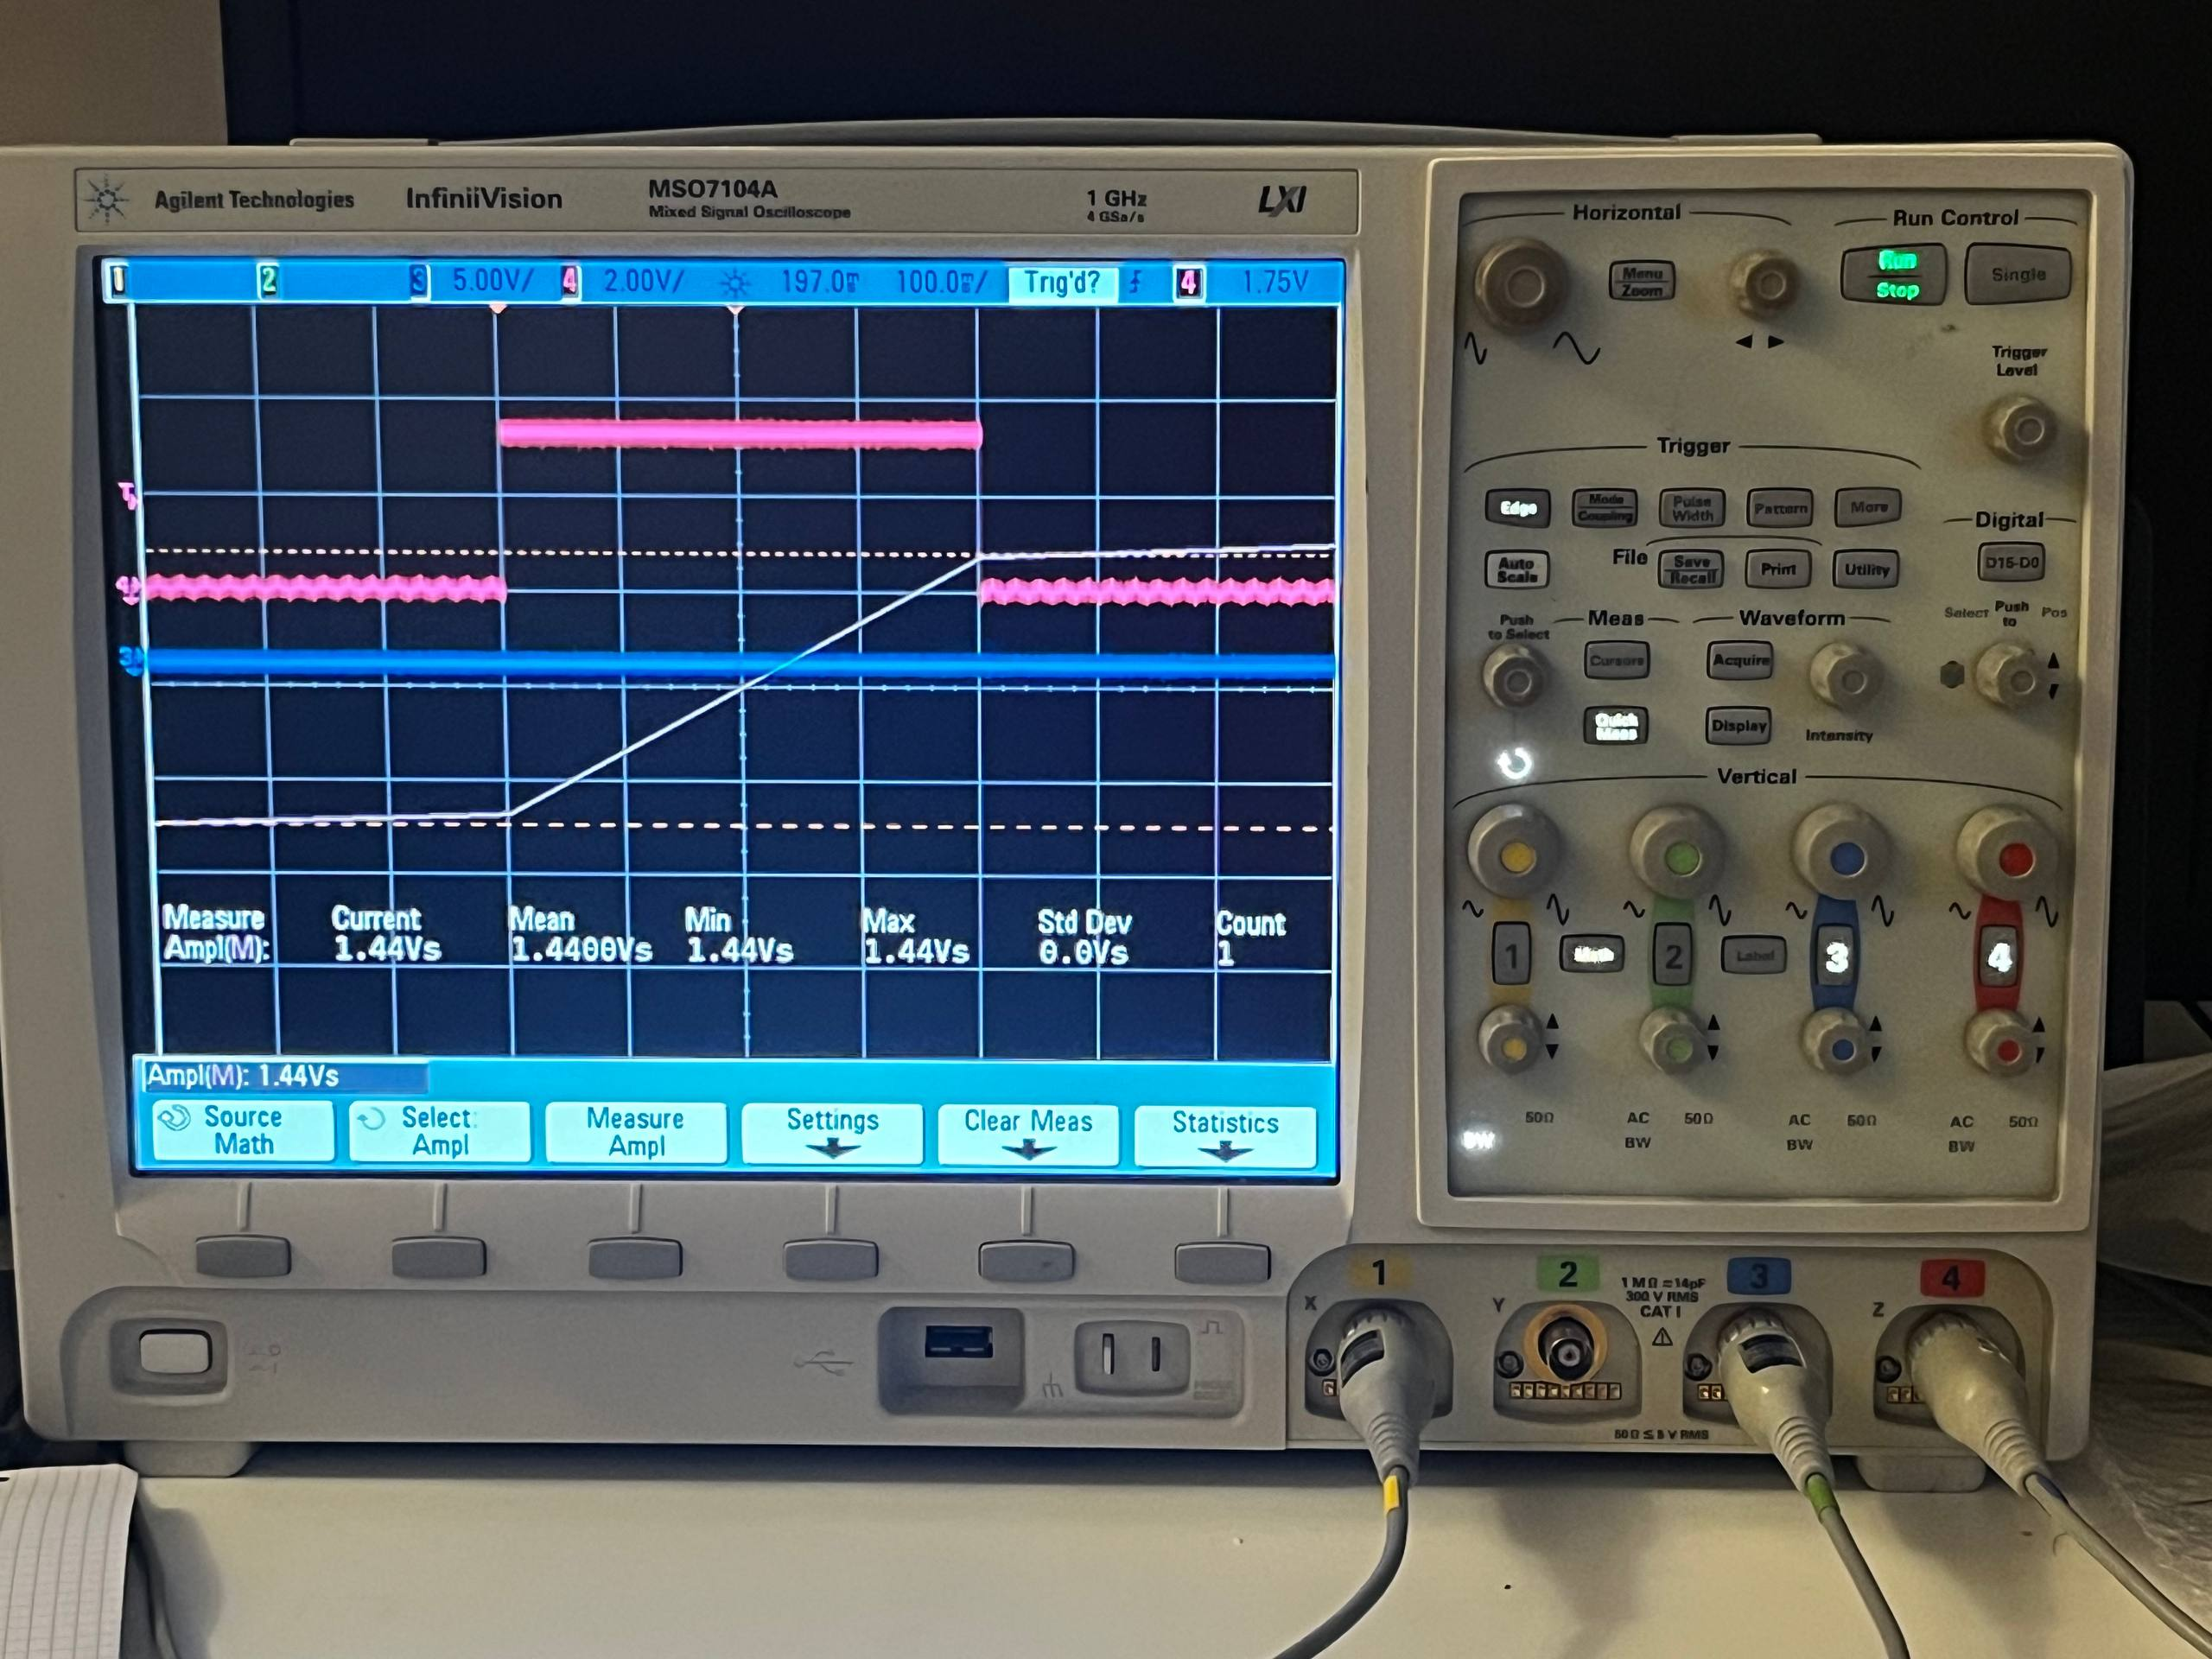
\includegraphics[width=0.62\textwidth]{images/oscilloscope.jpg}
			\caption{Oscilloscope setup used for electrical measurements during on-device energy benchmarking.}
			\label{fig:oscilloscope_energy_setup}
		\end{figure}
		
		\begin{figure}[H]
			\centering
			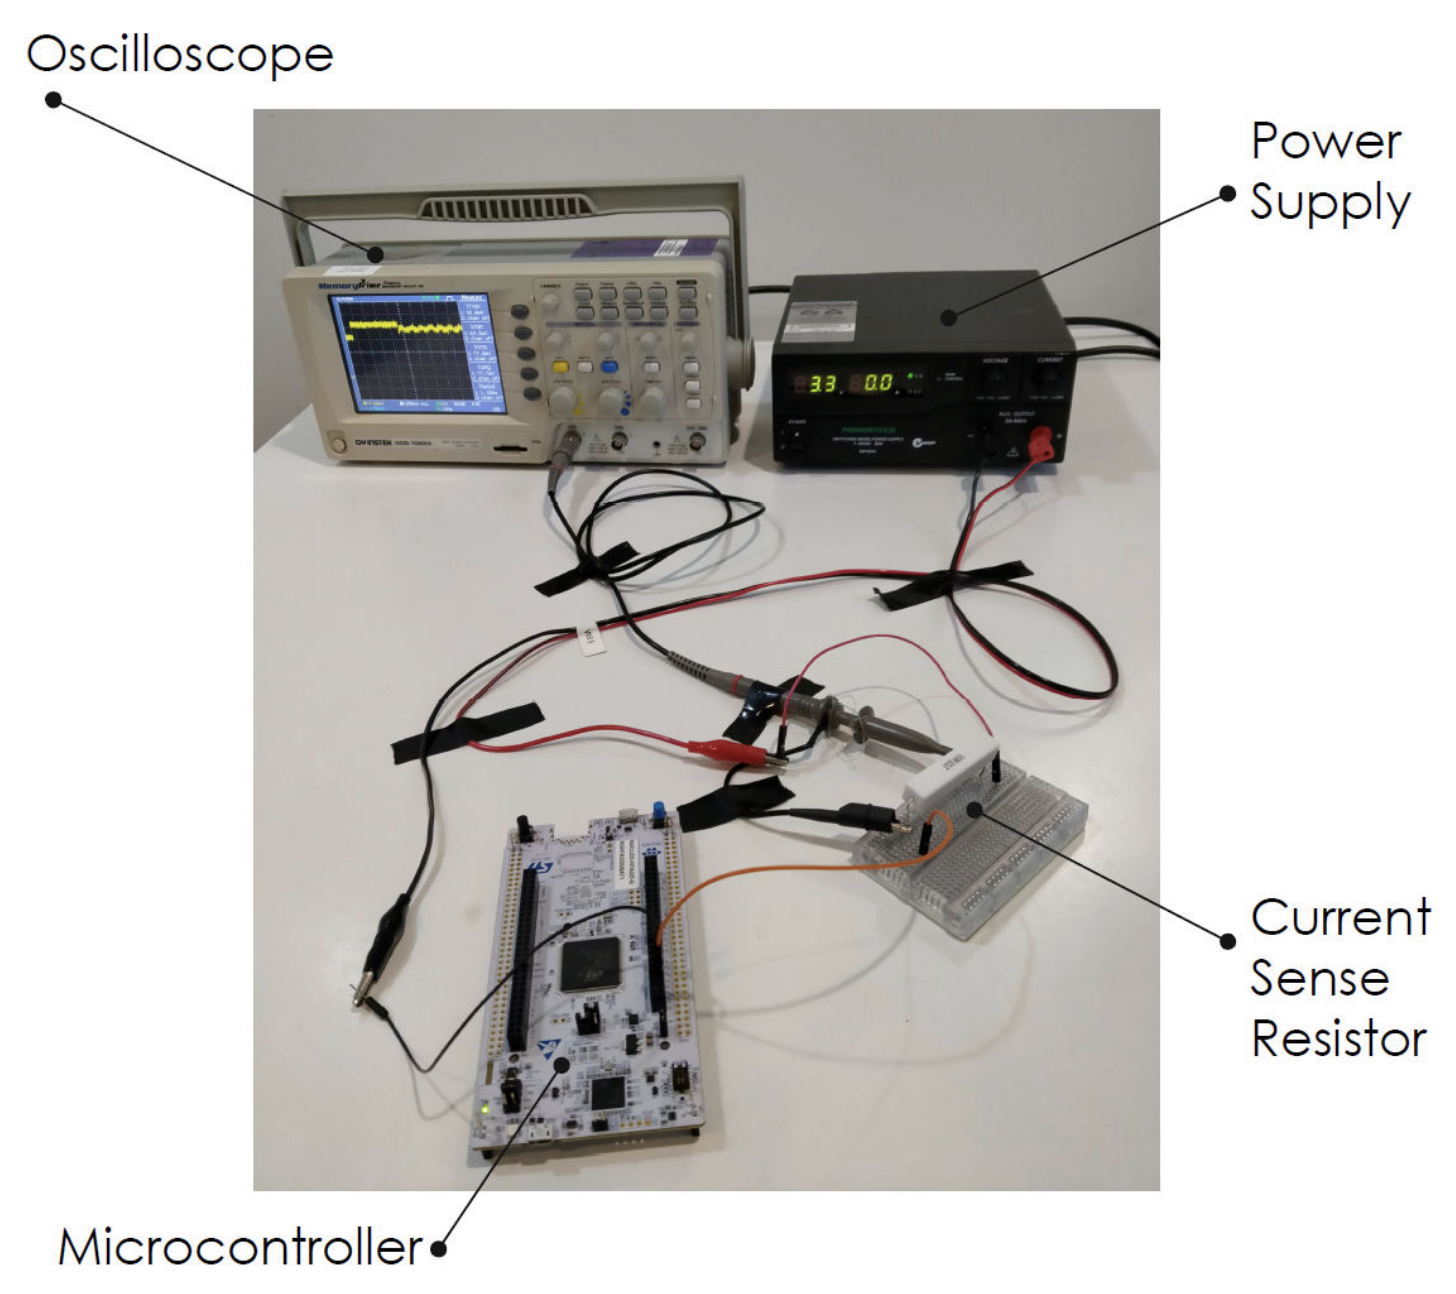
\includegraphics[width=0.62\textwidth]{images/measurement_example.png}
			\caption[Reference microcontroller energy-measurement setup.]{Reference example of a microcontroller energy-measurement setup, adapted from prior work on compression-aware bird-call inference benchmarking \cite{tao2022energy}.}
			\label{fig:measurement_example_setup}
		\end{figure}
	\end{samepage}

		\begin{sloppypar}
		Power and energy benchmarking follows the instrumentation strategy shown in Figures~\ref{fig:oscilloscope_energy_setup} and \ref{fig:measurement_example_setup}. The key metric is energy per inference window, because it directly determines battery lifetime in always-on monitoring. Results in Table~\ref{tab:energy_benchmark} show that the embedded pipeline reaches a substantially lower energy operating point than heavier baselines, even when absolute latency is higher.
		\end{sloppypar}

	The measured values show a clear scaling pattern. Relative to Raspberry Pi 3B+ student TFLite inference (\(0.1720\)~J per window), the AudioMoth deployment (\(0.0771\)~J) reduces energy per inference by about \(55\%\). Relative to the Raspberry Pi student STFT baseline (\(1.6500\)~J), the reduction is about \(95.3\%\), and relative to the BirdNET baseline (\(2.7900\)~J) it is about \(97.2\%\). In other words, in the tested configuration the microcontroller pipeline operates at approximately \(2.23\times\), \(21.4\times\), and \(36.2\times\) lower energy cost per decision than those three references, respectively.

	This result highlights the practical deployment trade-off: the microcontroller profile accepts slower per-window inference in exchange for dramatically reduced average power. AudioMoth inference time per 3-second window is longer (\(1.692\)~s) than Raspberry Pi execution, but average power is much lower (\(0.0456\)~W versus \(\sim2.7\)--\(2.84\)~W). For long-horizon field monitoring, this trade is favorable because maintenance interval and autonomy dominate operational cost.

	A useful operational normalization is daily inference energy under continuous 3-second windowing (\(28{,}800\) windows/day). Under this regime, the measured figures correspond to approximately \(0.617\)~Wh/day (AudioMoth), \(1.376\)~Wh/day (Raspberry Pi student TFLite), \(13.2\)~Wh/day (Raspberry Pi student STFT baseline), and \(22.3\)~Wh/day (Raspberry Pi BirdNET baseline). This gap is large enough to change deployment logistics in practice, especially in remote sites where battery replacement intervals dominate field cost.

	\chapter{Conclusions and Future Work}
	\section{Conclusions}
		\begin{sloppypar}
		The presented system demonstrates that multi-species bird sound classification can be implemented with a compact architecture while retaining strong practical accuracy. The combination of a semi-learnable front-end, causal convolutional encoding, recurrent temporal memory, and focal-distillation training provides a usable solution for acoustically heterogeneous field data.
		\end{sloppypar}

		\begin{sloppypar}
		Across experiments, the semi-learnable combined log--linear front-end consistently provides the best trade-off between flexibility and stability. It outperforms fixed mel and linear-triangular mappings in controlled comparisons, and it also outperforms a fully learnable front-end despite using a far more constrained parameterization. This result shows that structured adaptability can be more effective than unconstrained flexibility in low-footprint bioacoustic models.
		\end{sloppypar}

		\begin{sloppypar}
		Results on the full \(70(+1)\)-class setting confirm that the approach scales beyond small toy subsets. Larger models recover additional absolute accuracy, but the compact student remains competitive and preserves the deployment-oriented profile required for long-duration acoustic monitoring. The measured efficiency gap versus heavier baselines further supports this conclusion, with order-of-magnitude reductions in inference energy cost on comparable hardware classes and a BirdNET comparison that remains well above the \(16\times\) reference level.
		\end{sloppypar}

		The main methodological takeaway is that effective low-power bioacoustic classification emerges from the joint design and specialization of the data pipeline, spectral representation, temporal architecture, and training objective, rather than from isolated optimization of a single component.

		The measured energy profile has direct implications for field deployment. Under continuous 3-second windowing, the deployed system operates at approximately \(0.617\)~Wh/day, whereas the BirdNET reference benchmark is approximately \(22.3\)~Wh/day under the same normalization. Under an equal daily energy budget, one BirdNET-level node therefore corresponds to about 36 low-power deployed nodes, with clear impact on battery replacement intervals, storage planning, and the number of simultaneously monitored locations.

	\subsection{Limitations}
	Despite the positive results, several limitations remain explicit:
	\begin{itemize}
		\item the current formulation is closed-set classification with an explicit ``no bird'' class, so open-set behavior on unseen taxa is not solved in this work;
		\item dataset composition is geographically and acoustically biased by available sources, which may limit transfer without local adaptation;
		\item long-tail species with scarce or highly variable recordings remain more fragile than frequent classes;
		\item inference is single-label per window, so overlapping vocalizations from multiple species are not fully represented and require dedicated multi-label extensions;
		\item although the deployment stack was validated on the target hardware, the system was not yet evaluated in a full end-to-end field campaign with prolonged on-device operation under realistic environmental conditions; as a consequence, the present work demonstrates technical feasibility on device, but not yet full ecological validation under real deployment variability;
		\item the complete inference pipeline on AudioMoth remains relatively slow in absolute terms, even if its energy profile is favorable; the measured latency is still compatible with the current 3-second-window regime, but it leaves limited headroom for more demanding on-device logic, denser streaming schedules, or additional real-time processing stages;
		\item feedback exchanged with Open Acoustic Devices after this work indicated that accommodating edge inference more naturally on the platform would benefit from dedicated hardware and/or firmware revisions, rather than relying only on model-level optimization.
	\end{itemize}
	\section{Future Work}
	A key development direction is the \emph{Wren Framework}, currently under active implementation. The aim is to turn the methodology presented in this thesis into a reusable workflow that connects domain experts in biology, bioacoustics, and conservation practice with machine-learning pipelines, without requiring advanced ML engineering expertise for every new study.

	In this vision, users with strong domain knowledge can adapt the system by changing dataset composition, target species sets, and a controlled set of training and deployment parameters, while the underlying optimization and export pipeline remains stable and reproducible. The same framework can therefore support ad hoc models for different taxa, habitats, and monitoring objectives, including single-species detectors, regional multi-species classifiers, and subset-specialized models for difficult acoustic communities.

	A second major direction concerns late-stage information fusion across multiple devices. The objective would be to refine classification confidence by combining predictions generated at distinct spatial locations. In landscape-scale monitoring, species occurrences are not independently and identically distributed: they are structured by spatial context, habitat continuity, altitude, and broader ecological similarity between sites. As a result, detections from nearby or ecologically similar nodes can provide contextual evidence for one another. A distributed fusion layer could therefore improve reliability by reweighting local predictions in light of spatially and ecologically correlated observations, rather than treating each device as an isolated classifier.

	\begin{figure}[H]
		\centering
		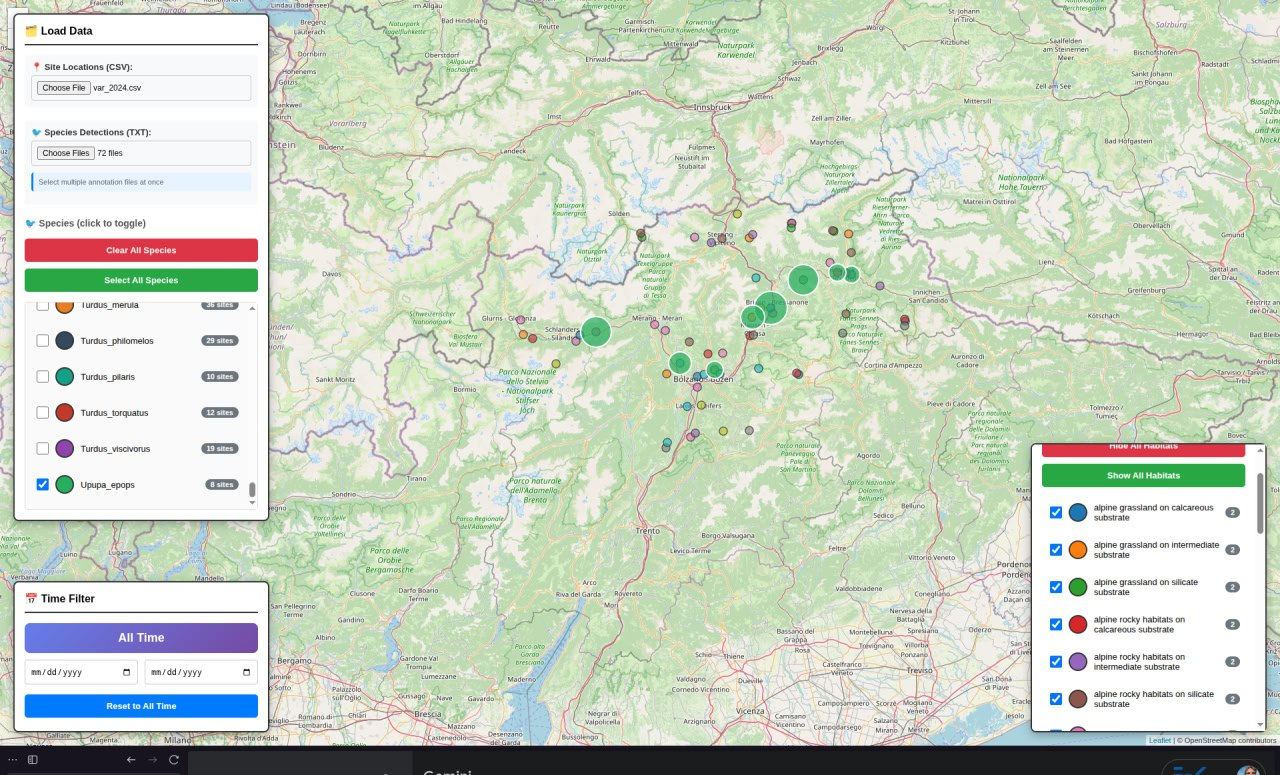
\includegraphics[width=0.72\textwidth]{images/map.jpg}
		\vspace{0.7em}
		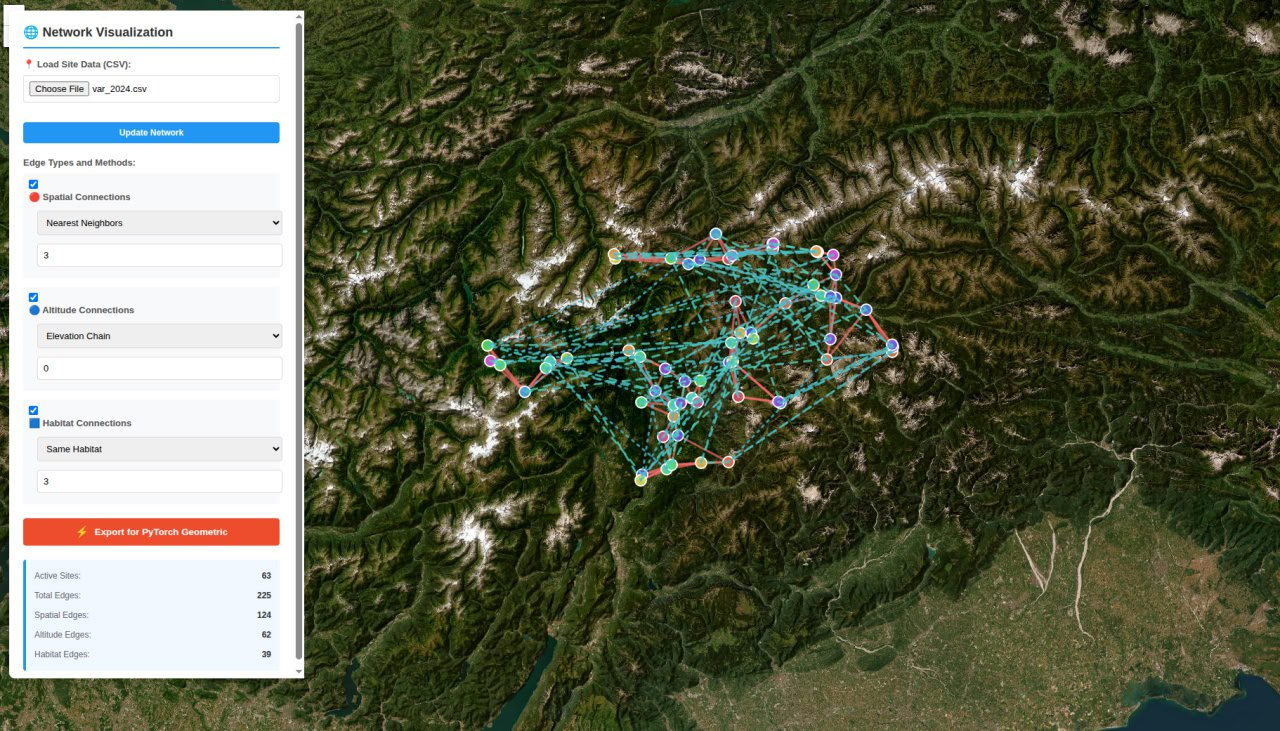
\includegraphics[width=0.72\textwidth]{images/map_2.jpg}
		\caption[Conceptual direction for multi-device ensemble monitoring.]{Conceptual direction for multi-device ensemble monitoring: coordinated nodes with subset-specialized models enabling geolocalized species mapping.}
		\label{fig:multi_node_ensemble_mapping}
	\end{figure}

	This collaborative direction also opens a direct path to spatial analytics, including near-real-time geolocalization maps of detections and temporal reconstruction of movement trajectories for selected species groups. In practical monitoring campaigns, this capability would move the system from single-point classification toward distributed ecological sensing and spatiotemporal interpretation.

	A further practical direction concerns platform evolution for native embedded inference support. In line with the technical feedback discussed above, future versions of the AudioMoth ecosystem may include hardware and/or firmware revisions explicitly aimed at accommodating edge inference more effectively. If this direction is realized, it would reduce current deployment bottlenecks and make the proposed class of low-power bioacoustic models easier to integrate, benchmark, and operate in the field.


		\begin{sloppypar}
		Additional research is required on robustness under real domain shift, including site transfer, seasonal drift, and changing background communities. This includes threshold-calibration studies for operational precision/recall control and deeper confusion analysis on difficult taxonomic groups.
		\end{sloppypar}

		\begin{sloppypar}
		A further direction is tighter end-to-end validation of exported low-precision inference. This means explicitly measuring the gap between floating-point validation metrics and deployed INT8 behavior under identical test streams and long-duration field conditions.
		\end{sloppypar}

		{\sloppy\printbibliography[heading=bibintoc]} % biblatex

	

	\end{document}
